\documentclass[a4paper,10pt]{article}

\usepackage[english]{babel}
\usepackage{graphicx}
\usepackage[colorlinks, allcolors=black]{hyperref}
\usepackage{geometry}
\geometry{tmargin=3cm, bmargin=2.2cm, lmargin=2.2cm, rmargin=2cm}
\usepackage{todonotes} %Used for the figure placeholders
\graphicspath{{Images/}}
\usepackage{placeins}

% Your name and student number must be filled in on the title page found in
% titlepage.tex.

\begin{document}
\begin{titlepage}
    \newpage
    \thispagestyle{empty}
    \frenchspacing
    \hspace{-0.2cm}
    
\includegraphics[height=3.4cm]{sedes}
    \hspace{0.2cm}
    \rule{0.5pt}{3.4cm}
    \hspace{0.2cm}
    \begin{minipage}[b]{8cm}
        \Large{Katholieke\newline Universiteit\newline Leuven}\smallskip\newline
        \large{}\smallskip\newline
        \textbf{Department of\newline Computer Science}\smallskip
    \end{minipage}
    \hspace{\stretch{1}}
    \vspace*{3.2cm}\vfill
    \begin{center}
        \begin{minipage}[t]{\textwidth}
            \begin{center}
                \LARGE{\rm{\textbf{\uppercase{Document Processing}}\\ADD
                application}}\\
                \Large{\rm{Software Architecture (H09B5a and H07Z9a) -- 
                Part 2a}}
            \end{center}
        \end{minipage}
    \end{center}
    \vfill
    \hfill\makebox[8.5cm][l]{%
        \vbox to 7cm{\vfill\noindent
            {\rm \textbf{Student A (r123456)}}\\
            {\rm \textbf{Student B (r987654)}}\\[2mm]
            {\rm Academic year 2014--2015}
        }
    }
\end{titlepage}


\tableofcontents
\newpage

\section{Introduction}\label{sec:introduction}
The goal of this project was to design a document processing system. In this document, we describe the final architecture, which was designed based on the requirements from the domain analysis and the priorities of these requirements given by our stakeholders. The provided initial architecture was used as a starting point to achieve this.
Section \ref{sec:overview} lists the architectural decisions for all non-functional requirements and discusses the final architecture.
Section \ref{sec:client-server} provides and discusses the main context and decomposition diagrams of our architecture (i.e. the context and primary diagram of the component-and-connector view) along with a discussion of the main architectural decisions involved.
Section \ref{sec:decomposition} provides and discusses the more fine-grained decompositions of some of the major components in the main decomposition.
Section \ref{sec:deployment} provides and discusses the deployment of the components of the component-and-connector view on physical nodes.
Finally, Section \ref{sec:scenarios} illustrates how our architecture accomplishes the most important functionality and data flows using sequence diagrams.
Afterwards, Appendix \ref*{app:catalog} lists and describes all components of the component-and-connector view and their interfaces and Appendix \ref*{app:datatypes} lists and describes the data types used in these interfaces.
\section{Overview}\label{sec:overview}
This section gives a high-level but complete overview of the system: it lists the design decisions for all non-functional requirements and provides a discussion concerning the strong and weak points of the architecture.
\subsection{Architectural decisions}
In this section, we give an overview of the architectural decisions made in our architecture in order to achieve the requirements given in the domain analysis and the residual drivers given in the provided initial architecture. However, we will not repeat any decisions that were already documented in this provided initial architecture as they can be found there.

\paragraph{Av1a \& Av2a\@: Notifying the appropriate operator within 1 minute}
\textit{Av1a} and \textit{Av2a} require the system to notify the eDocs operator within 1 minute in case of failure of the internal infrastructure responsible for generating documents or the internal (sub-)system responsible for storing documents in personal document stores. To achieve this, the \texttt{NotificationHandler} handles all incoming notifications and forwards those that are destined for an eDocs operator to the \texttt{EDocsAdminFacade}, which in turn delivers these to the external \texttt{EDocsAdminClient}. To ensure that notifications get sent to the eDocs operator in a timely fashion, both the \texttt{EDocsAdminFacade} and the \texttt{NotificationHandler} are deployed on the same node, which is separated from all other nodes to increase performance.\\
For more details, we refer to Section \ref{subsubsec:Av1a-Av2a} and Section \ref{sec:deployment}.

\paragraph{Av1b\@: Storing the status of an individual job}
\textit{Av1b} requires the system to store the status of an individual job. To achieve this, the \texttt{JobManager} accepts all read and write requests regarding the storage of job data, including status information.\\
For more details, we refer to Section \ref{subsubsec:Av1b} and Section \ref{subsec:decomp-JobManager}.

\paragraph{Av2b\@: Temporary storage and user notification upon PDSDB failure}
\textit{Av2b} requires (1) documents that should be delivered via the personal document store to be cached for at least 3 hours in case of unavailability and (2) a clear message to be provided to the recipient in this case. To achieve this, we introduced the \texttt{DocumentStorageCache}: this component temporarily stores the \texttt{DocumentIds} and corresponding \texttt{RecipientIds} of all generated documents that are to be delivered to the \texttt{PDSDB} during downtime of the latter component up to a maximum of 3 hours. When the \texttt{PDSDB} turns operational again, it notifies the \texttt{DocumentStorageManager} with a sign of life, which in turn retrieves all documents and their corresponding meta data from the \texttt{DocumentDB} using the previously mentioned ids and subsequently stores them in the \texttt{PDSDB} after conversion of the \texttt{DocumentMetaData}.\\
Note that the user therefore perceives a maximum total downtime of 3 hours and that the \texttt{RecipientFacade} is in charge of presenting the user with a clear error message after having performed a read request in his or her behalf that has failed due to the unavailability of the \texttt{PDSDB}. However, during the time needed for the \texttt{DocumentStorageManager} to transfer all documents and meta data that the cached ids refer to, it is possible that the user is not able to access (part of) his or her documents via the \texttt{PDSDB}, more specifically those that are still being transferred. Since the requirements do not demand the user to be able to regain full functionality of his or her personal document store at once, finding a better alternative for this gradual revival of the \texttt{PDSDB} is out of scope.\\
Finally, we would like to stress that the \texttt{DocumentStorageManager} and the \texttt{PDSDB} are necessarily deployed on different nodes for the former to be able to do its caching job while the latter is not operational during downtime. More precisely, the \texttt{DocumentStorageManager} implicitly pings the \texttt{PDSDB} when storing document data in it. The echo message then, in turn, consists of the write confirmation that is subsequently received. If one of those writes should fail, all subsequent writes are internally converted into pairs of \texttt{DocumentId}-\texttt{RecipientId} writes to the aforementioned cache. Once the \texttt{PDSDB} is operational again and all cached ids are processed, subsequent writes to the \texttt{PDSDB} will no longer be redirected through the \texttt{DocumentStorageCache}.\\
For more details, we refer to Section \ref{subsubsec:Av2b}, Section \ref{subsec:decomp-DocumentStorageFunctionality} and Section \ref{sec:deployment}.

\paragraph{Av3\@: Zoomit failure}
\textit{Av3} requires the system to be able to (1) autonomously detect when an invoice is not accepted by Zoomit, (2) temporarily store at least 2 days of these invoices locally until they are accepted by Zoomit, (3) keep on retrying to deliver a failed invoice to Zoomit in a proper fashion and (4) notify an eDocs operator after 5 failed attempts of at least 10 different invoices. To achieve this, the \texttt{ZoomitFacade} is able to receive a delivery confirmation from the \texttt{ZoomitChannel} (i.e. the invoice was accepted by Zoomit). Furthermore, the \texttt{ZoomitDeliveryCache} caches all \texttt{Documents} and corresponding \texttt{DeliveryInfo} for which the \texttt{ZoomitFacade} did not (yet) receive a delivery confirmation up to a maximum of 2 days of documents.\\
The \texttt{ZoomitFacade} then periodically retries to deliver the next document in the cached list of \texttt{Document}-\texttt{DeliveryInfo} pairs (note that the \texttt{ZoomitDeliveryCache} thus stores its entries in a circular manner) to the \texttt{ZoomitChannel} in a proper fashion by using exponential back-off. Once the \texttt{ZoomitFacade} has received a delivery confirmation regarding one of those cached documents, the corresponding \texttt{Document}-\texttt{DeliveryInfo} pair is deleted from the \texttt{ZoomitDeliveryCache} and the \texttt{ZoomitFacade} tries to deliver every other document in the list to the \texttt{ZoomitChannel} right after, disregarding the previously employed method of exponential back-off (because the external \texttt{ZoomitChannelNode} on which the \texttt{ZoomitChannel} resides, is now presumed to be operational again).\\
Finally, the \texttt{Document}-\texttt{DeliveryInfo} pairs in the \texttt{ZoomitDeliveryCache} need to be stored along with a counter that the \texttt{ZoomitFacade} increments after each failed attempt to send the respective document. Additionally, the \texttt{ZoomitFacade} keeps track of all cached pairs whose counters have reached the value of 5 and sends a notification to an eDocs operator through the \texttt{NotificationHandler}.
For more details, we refer to Section \ref{subsubsec:Av3}, Section \ref{subsubsec:Av1a-Av2a}, Section \ref{subsec:decomp-DeliveryFunctionality} and Section \ref{sec:deployment}.

\paragraph{P2\@: Document lookups}
\textit{P2} requires the system to be able to (1) respond to all incoming document requests in a timely fashion, (2) throttle excessive requests when the arrival rate is larger than a certain request specific value (determined by the requirements) so that the non-excessive ones continue to be handled in a timely fashion and (3) make sure that the performance of all other functionality of the system remains unaffected in case of a large number of requests. To achieve this, all potential bottleneck components that support the document lookup process are deployed on separate nodes. More precisely, the \texttt{RecipientFacade} and the \texttt{LinkMappingFunctionality} both reside on the same exclusive node as to increase the performance of these components and the communication between them (i.e. when a recipient has presented the former component with a link for which it has to determine the document it maps to). Both the \texttt{AuthenticationHandler} and the \texttt{SessionDB} are also deployed on the same individual node as to not let the authentication subprocess decrease the performance of the document lookup process. The \texttt{PDSFacade} is deployed on the \texttt{PDSDBManagerNode} (discussed in the provided initial architecture), along with the \texttt{PDSLongTermManager} and the two \texttt{PDSReplicationManagers}, as to increase communication performance between this \texttt{PDSFacade} and the \texttt{PDSDB} supercomponent. Notice that \textit{Av1} already demands the \texttt{PDSDB} to be deployed separate from all other functionality according to the provided initial architecture and that \textit{P2} can rely on this design decision to deliver an optimally increased (taking the availability constraints of \textit{Av1} into account) performance of this supercomponent.\\
Because the \texttt{DocumentDB}, like the \texttt{PDSDB}, stores a large amount of documents and correspondingly handles a large amount of document requests, its documents are partitioned across several \texttt{DocumentDBShards} that each reside on their own \texttt{DocumentDBShardNode}. This sharding technique results in a performance increase that is statistically equivalent to the one that is achieved by active replication, but it is significantly less costly regarding storage costs (which is more of a concern for documents than for other kinds of data). In order to further increase performance of the \texttt{DocumentDB}, the \texttt{DocumentDBShardingManager}, which is in charge of managing all \texttt{DocumentDBShards} and forwarding read and write requests to the appropriate ones, is also deployed on an individual node.\\
Finally, both the \texttt{DocumentDB} and the \texttt{PDSDB} have the ability to throttle excessive read requests from the \texttt{RecipientFacade} (all other requests remain unaffected) when the rate of these incoming requests exceeds a certain request specific value (determined by the requirements). Also note that the performance of all other functionality of the system remains unaffected even at this maximum, since all potential bottleneck components that support the document lookup process are deployed on separate nodes, effectively increasing their performance (as discussed above) and thereby providing both an increased level of performance for the document lookup process and a sufficient level of performance for all other functionality.
For more details, we refer to Section \ref{subsubsec:P2}, Section \ref{sec:client-server}, Section \ref{subsec:decomp-UserFunctionality}, Section \ref{subsec:decomp-PDSDB}, Section \ref{subsec:decomp-DocumentDB} and Section \ref{sec:deployment}.

\paragraph{P3\@: Status overview for customer administrators}
\textit{P3} requires (1) the status overview of all document processing jobs initiated by a certain customer organization to be delivered to the respective customer administrator(s) in a timely fashion (i.e. the provided status of a document processing job should be consistent up to 1 minute ago) and (2) the construction of this status overview not to hinder other parts of the system. To achieve this, all potential bottleneck components that support the status overview process are deployed on separate nodes as to increase their performance. More precisely, both the \texttt{AuthenticationHandler} and the \texttt{SessionDB} are also deployed on the same individual node as to not let the authentication subprocess decrease the performance of the status overview process. Furthermore, the \texttt{CustomerOrganizationFacade} and the \texttt{JobManager} supercomponent are also deployed separate from all other components in the system. More specifically, the former occupies a single node by itself, while the latter is responsible for storing all jobs, which are partitioned across several \texttt{JobDBShards} that each reside on their own \texttt{JobDBShardNode} too. This sharding technique results in a performance increase that is statistically equivalent to the one that is achieved by active replication, but it is less costly regarding storage costs. In order to further increase performance of the \texttt{JobManager} and the corresponding speed at which job statuses can be requested, the \texttt{JobDBShardingManager}, which is in charge of managing all \texttt{JobDBShards} and forwarding read and write requests to the appropriate ones, is also deployed on an individual node.\\
Note that the performance of all other functionality of the system remains unaffected during the construction of such a status overview, since all potential bottleneck components that support this status overview process are deployed on separate nodes, effectively increasing their performance (as discussed above) and thereby providing both an increased level of performance for the status overview process and a sufficient level of performance for all other functionality.\\
Also note that the \texttt{JobDBShardManager} and corresponding \texttt{JobDBShards} do not distinguish between jobs of different age during the construction of an overview. Although the requirements mention a different minimal response time for each type of job with regard to its age, our system does not offer this distinction. Instead, the \texttt{JobDBShardManager} and corresponding \texttt{JobDBShards} simply present the customer administrator(s) with a response time that is equal to the lowest of all minimal response times mentioned in the requirements. This strategy was chosen due to the fact that (1) different dynamic storage requirements for jobs along with their periodical synchronization would largely outweigh this simple storage approach with respect to implementation and deployment costs and (2) the same level of performance per type of job can easily be provided by this simple storage approach (i.e. the uniform response time per job is equal to lowest of all minimal response times) because of the small storage capacity that is needed for job data.
For more details, we refer to Section \ref{subsubsec:P3}, Section \ref{subsec:decomp-UserFunctionality}, Section \ref{subsec:decomp-JobManager} and Section \ref{sec:deployment}.

\paragraph{M1\@: New type of document: bank statements}
\textit{M1} requires (1) the interface for initializing document processing jobs to be easily extendible with the functionality to provide the raw data for other types of documents, (2) the interface for registering companies to be easily extendible with the functionality to enable the new types of documents for new customer organizations and configure their template for these types of documents, (3) the functionality for generating documents to be easily extendible with the new generation steps for the new types of documents, (4) the generation of the new types of documents to reuse as much of the existing functionality for generating documents as possible, (5) the storage of generated documents of the new types of documents not to require any changes to the existing system for storing generated documents and (6) the interface for consulting the personal document store and specific documents to be easily extendible with the functionality to show the new types of documents. To achieve this, all relevant interfaces of the components involved in the data flows of these processes, including the specified data types, are generic enough to cope with different document types. Furthermore, all potential changes are encapsulated by the \texttt{RawDataHandler} and the \texttt{DocumentGenerationManager} supercomponent. More specifically, the former will now also need to handle the verification of raw data that is characteristic for these new types of documents. The generic internal structure of the latter also ensures that the generation of new document types will reuse as much of the existing functionality for generating documents as possible. Note that the type and the format of a document are two different things: the first being the focus of \textit{M1} and the second being the internal structure of a \texttt{Document} data type, which remains untouched in the context of \textit{M1}. Since the \texttt{RecipientFacade} only has knowledge about the latter, no changes need to be made to the \texttt{RecipientFacade} upon introduction of a new document type.
For more details, we refer to Section \ref{subsubsec:M1}, Section \ref{sec:client-server}, Section \ref{subsec:decomp-DocumentGenerationManager}, Section \ref{subsec:decomp-UserFunctionality} and Appendix \ref*{app:datatypes}.

\paragraph{M2\@: Multiple print \& postal services}
\textit{M2} requires (1) the system to be able to easily switch print \& postal service in the future, (2) the incorporation of this new print \& postal service in the system to only affect the final steps of the document processing flow. To achieve this, the \texttt{Print\&PostalServiceFacade} encapsulates all changes that might need to be made in order to seamlessly incorporate a new print \& postal service in the system, e.g. additional methods, external interfaces, \dots
For more details, we refer to Section \ref{subsubsec:M2} and Section \ref{subsec:decomp-DeliveryFunctionality}.

\paragraph{M3\@: Dynamic selection of the cheapest of print \& postal services}
\textit{M3} requires the system to be easily extendible in order to be able to (1) employ multiple print \& postal services across the world, (2) receive the daily price and capacity of each print \& postal service and (3) dynamically select (i.e. on a daily basis) the most suited print \& postal service based on the system's document processing load, the price of the service and the location to which the documents should be sent. To achieve this, the \texttt{Print\&PostalServiceFacade} encapsulates all changes that might need to be made in order to seamlessly incorporate this new functionality in the system. More precisely, this component will only require (1) an additional external interface to each of the employed print \& postal services, (2) an internal interface to the \texttt{OtherDB} to consult all SLAs in order to retrieve the approximate location and size of all batches for the day and (3) its internal structure to be adapted to the new functionality.
For more details, we refer to Section \ref{subsubsec:M3} and Section \ref{subsec:decomp-DeliveryFunctionality}.

\subsection{Discussion}
GEEN JOBFACADE MEER
Use this section to discuss your architecture in retrospect.
For example, what are the strong points of your architecture?
What are the weak points? Is there anything you would have done otherwise with
your current experience?
Are there any remarks about the architecture that you would give to your
customers?
Etc.

\section{Client-server view (UML Component diagram)}\label{sec:client-server}
\paragraph{Context diagram}
The context diagram of the component-and-connector view is given in Figure \ref{fig:cc-context}. As shown, six distinct types of external components communicate with the system:
(i) the EDocsAdminClient represents a client device of an administrator of eDocs that communicates with the eDocs System,
(ii) the CustomerOrganizationClient represents a client device of a Customer Organization (i.e. Customer Administrator and Customer Information System) that communicates with the eDocs System,
(iii) the RecipientClient represents a client device of an unregistered or registered recipient of eDocs that communicates with the eDocs System,
(iv) the ZoomitChannel represents the servers of Zoomit to which documents can be sent for further delivery,
(v) the Print\&PostalServiceChannel represents the servers of a print \& postal service to which documents can be sent for further delivery,
(vi) the EmailChannel represents a mail server of an e-mail provider to which documents can be sent for further delivery.
Notice that each external interface on the client side is provided by a separate facade component and that each delivery channel interfaces with the \texttt{DeliveryFunctionality} component.

\begin{figure}[!htp]
	\centering
	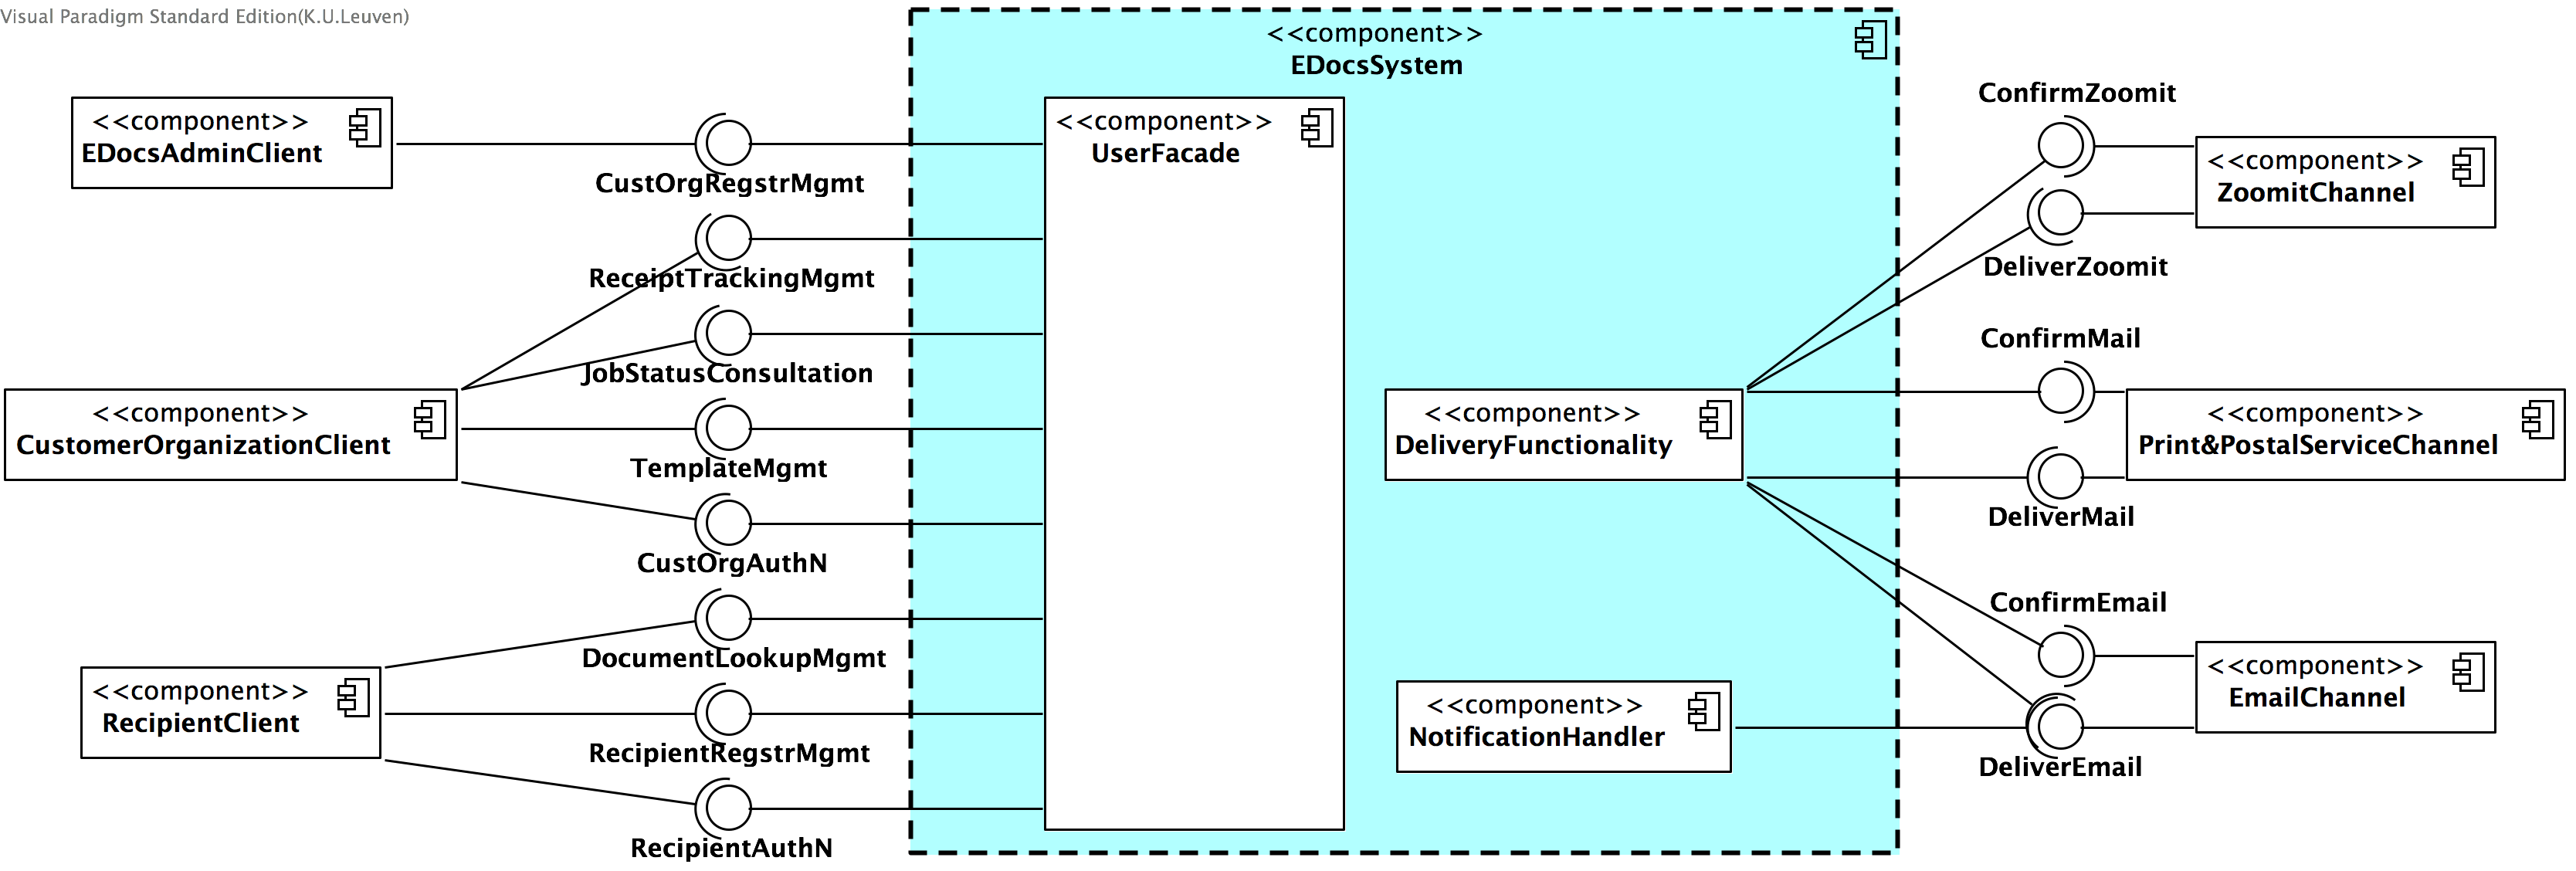
\includegraphics[width=0.8\textwidth]{ContextDiagram.png}
	\caption{Context diagram for the client-server view.}
	\label{fig:cc-context}
\end{figure}
\FloatBarrier

\paragraph{Primary diagram}
The main component-and-connector view is shown in Figure \ref{fig:cs-primary}. All components that were decomposed further are highlighted. The DeliveryFunctionality is further decomposed in Section \ref{subsec:decomp-DeliveryFunctionality}, the DocumentDB in Section \ref{subsec:decomp-DocumentDB}, the DocumentGenerationManager in Section \ref{subsec:decomp-DocumentGenerationManager}, the DocumentStorageFunctionality in Section \ref{subsec:decomp-DocumentStorageFunctionality}, the JobManager in Section \ref{subsec:decomp-JobManager}, the LinkMappingFunctionality in Section \ref{subsec:decomp-LinkMappingFunctionality}, the PDSDB in Section \ref{subsec:decomp-PDSDB} and the UserFunctionality in Section \ref{subsec:decomp-UserFunctionality}. The descriptions of all components in Figure \ref{fig:cs-primary}, their sub-components and their interfaces are given in Appendix \ref*{app:catalog}.

\begin{figure}[!htp]
	\centering
	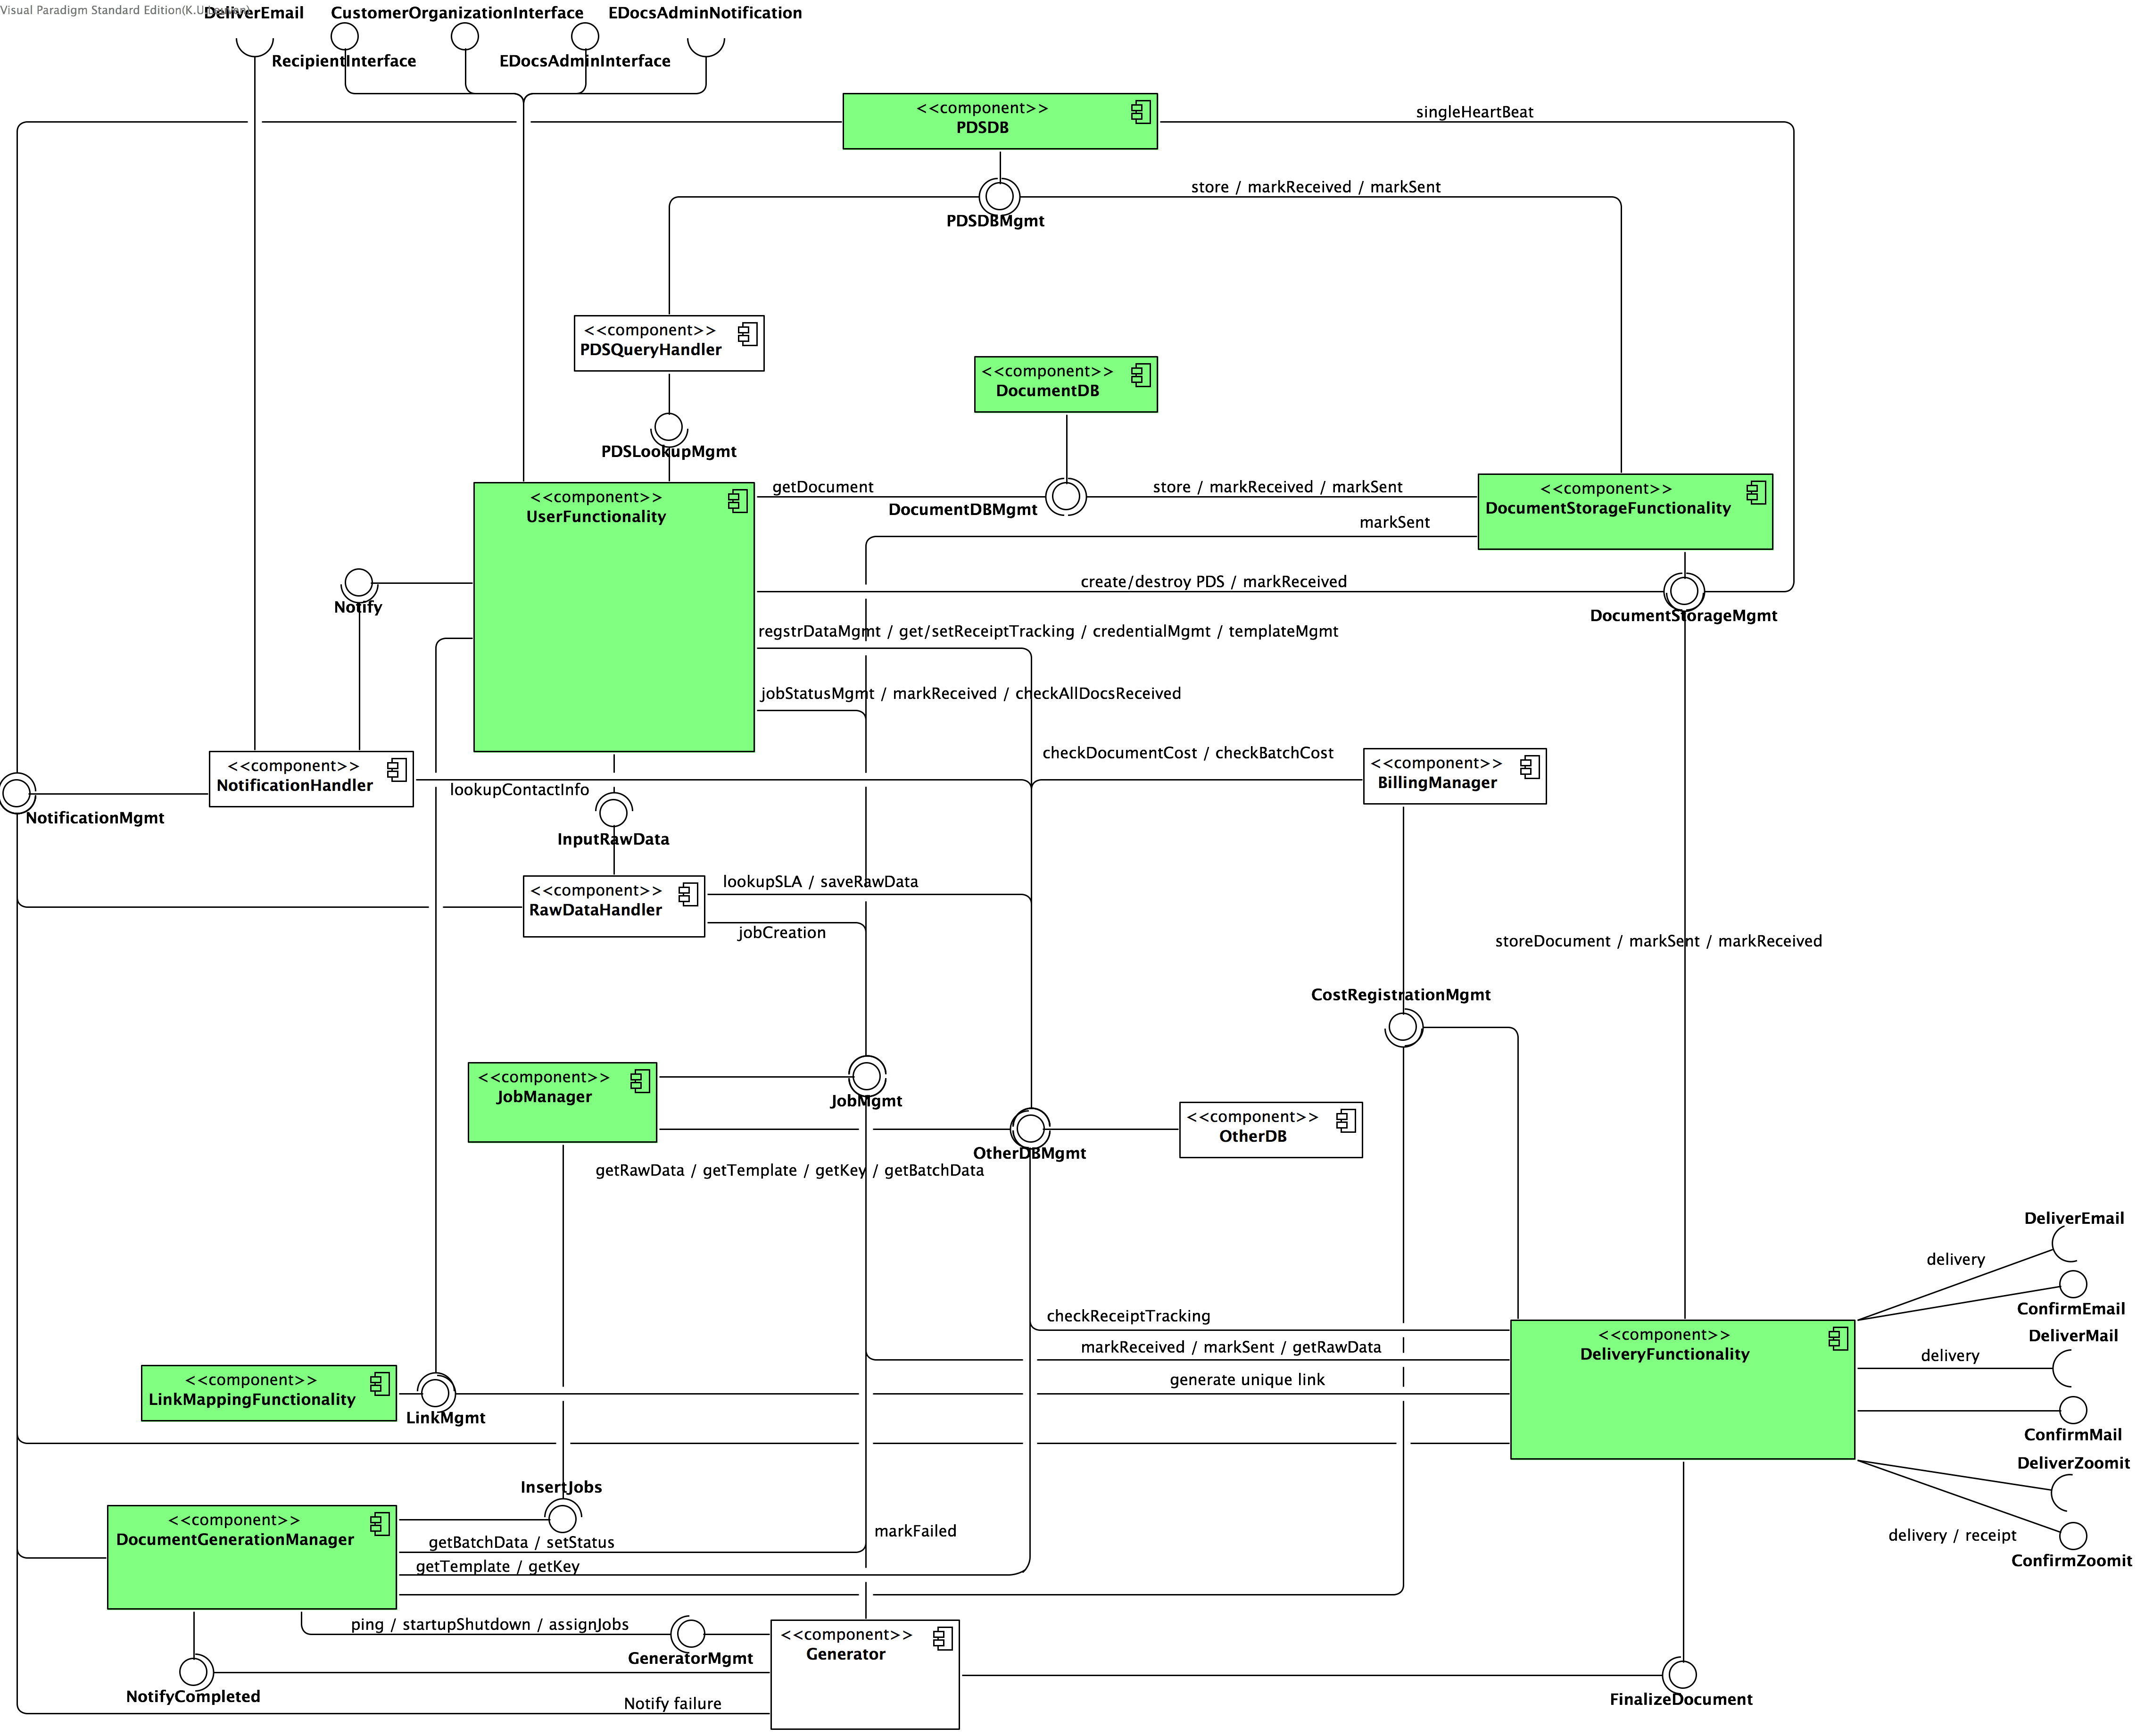
\includegraphics[width=0.8\textwidth]{ClientServerView.png}
	\caption{Primary diagram of the client-server view.}
	\label{fig:cs-primary}
\end{figure}
\FloatBarrier

\subsection{Main architectural decisions}
Figure \ref{fig:cs-primary} provides the overall description of the architecture and illustrates the most important architectural decisions for achieving the required qualities. Here we document how our architecture fulfils the most important qualities (based on the priorities given by the stakeholders). Although the qualities that were already discussed in the provided initial architecture will not be analysed any further here, their residual drivers will. The resulting qualities thus consist of Av1a \& Av2a: Notifying the appropriate operator within 1 minute, Av1b: Storing the status of an individual job and Av2b: Temporary storage and user notification during PDSDB failure. In addition, we also highlight P2: Document lookups, because of the importance of this quality to a significant part of the recipient base.

\subsubsection{Av1a \& Av2a\@: Notifying the appropriate operator within 1 minute}\label{subsubsec:Av1a-Av2a}
Firstly, \textit{Av1a} and \textit{Av2a} require the system to notify the eDocs operator in case of failure of the internal infrastructure responsible for generating documents or the internal (sub-)system responsible for storing documents in personal document stores (cf. the analysis of \textit{Av1} and \textit{Av2} in the provided initial architecture respectively). Therefore, the \texttt{NotificationHandler} handles all incoming notifications from the respective components (i.e. the \texttt{DocumentGenerationManager} and the \texttt{PDSDB}) and forwards those that are destined for an eDocs operator to the \texttt{EDocsAdminFacade}, which in turn delivers these to the external \texttt{EDocsAdminClient}.

Secondly, to ensure that notifications get sent to the eDocs operator in a timely fashion (i.e. within 1 minute), both the \texttt{EDocsAdminFacade} and the \texttt{NotificationHandler} are deployed on the same node, which is separated from all other nodes to increase performance (see the deployment view in Section \ref{sec:deployment}). As was already pointed out and discussed in the provided initial architecture, it is the responsibility of the \texttt{DocumentGenerationManager} and the \texttt{PDSDB} that the \texttt{NotificationHandler} itself gets notified in a timely fashion.

The \texttt{DocumentGenerationManager} and the \texttt{PDSDB} are further decomposed in Sections \ref{subsec:decomp-DocumentGenerationManager} and \ref{subsec:decomp-PDSDB} respectively.
\subsubsection*{Alternatives considered}
\paragraph{Alternative(s) for choice 1} Explain what alternative(s) you
considered for this design choice and why they where not selected.

\subsubsection{Av1b\@: Storing the status of an individual job}\label{subsubsec:Av1b}
\textit{Av1b} requires the system to store the status of an individual document processing job in order to be able to show the status of the jobs affected by the failure of the internal infrastructure responsible for generating documents (cf. the analysis of \textit{Av1} in the provided initial architecture). To achieve this, the \texttt{JobManager} accepts all read and write requests regarding the storage of job data, including status information.
\subsubsection*{Alternatives considered}
\paragraph{Alternative(s) for choice 1} Explain what alternative(s) you
considered for this design choice and why they where not selected.

\subsubsection{Av2b\@: Temporary storage and user notification upon PDSDB failure}\label{subsubsec:Av2b}
Firstly, \textit{Av2b} requires documents that should be delivered via the personal document store to be cached for at least 3 hours in case of unavailability (cf. the analysis of \textit{Av2} in the provided initial architecture). Therefore, we introduced the \texttt{DocumentStorageFunctionality}: the \texttt{DocumentStorageCache} that is part of this component temporarily stores the \texttt{DocumentIds} and corresponding \texttt{RecipientIds} of all generated documents that are to be delivered to the \texttt{PDSDB} during downtime of the latter component up to a maximum of 3 hours. When the \texttt{PDSDB} turns operational again, it notifies the \texttt{DocumentStorageManager} (which is also a subcomponent of the \texttt{DocumentStorageFunctionality}) with a sign of life, which in turn retrieves all documents and their corresponding meta data from the \texttt{DocumentDB} using the previously mentioned ids and subsequently stores them in the \texttt{PDSDB} along with the converted \texttt{DocumentMetaData} (i.e. the original \texttt{DocumentMetaData}, including the corresponding \texttt{RecipientId} but omitting the \texttt{Email} if present). Note that the \texttt{DocumentStorageManager} and the \texttt{PDSDB} are necessarily deployed on different nodes for the former to be able to do its caching job while the latter is not operational during downtime (see the deployment view in Section \ref{sec:deployment}). More precisely, the \texttt{DocumentStorageManager} implicitly pings the \texttt{PDSDB} when storing document data in it. The echo message then, in turn, consists of the write confirmation that is subsequently received. If one of those writes should fail, all subsequent writes are internally converted into pairs of \texttt{DocumentId}-\texttt{RecipientId} writes to the aforementioned cache. Once the \texttt{PDSDB} is operational again and all cached ids are processed, subsequent writes to the \texttt{PDSDB} will no longer be redirected through the \texttt{DocumentStorageCache}.

Secondly, \textit{Av2b} requires a clear message to be provided to the recipient in case of unavailability of the personal document store. This responsibility is delegated to the \texttt{RecipientFacade} in the following way: this component presents the user with a clear error message after having performed a read request in his or her behalf that has failed due to the unavailability of the \texttt{PDSDB}. Note that the user therefore perceives a maximum total downtime of 3 hours. However, during the time needed for the \texttt{DocumentStorageManager} to transfer all documents and meta data that the cached ids refer to, it is possible that the user is not able to access (part of) his or her documents via the \texttt{PDSDB}, more specifically those that are still being transferred. Since the requirements do not demand the user to be able to regain full functionality of his or her personal document store at once, finding a better alternative for this gradual revival of the \texttt{PDSDB} is out of scope.

The \texttt{DocumentStorageFunctionality} is further decomposed in Section \ref{subsec:decomp-DocumentStorageFunctionality}.
\subsubsection*{Alternatives considered}
\paragraph{Alternative for DocumentStorageCache}
We could just as well do without the previously introduced \texttt{DocumentStorageCache} by letting the \texttt{DocumentStorageManager} actively look for documents in the \texttt{DocumentDB} that are not yet, but should be, present in the \texttt{PDSDB} upon revival of the \texttt{PDSDB}. A clear advantage of this approach is that the downtime of the \texttt{PDSDB} component is no longer restricted by the aforementioned 3-hour cache. An important disadvantage, however, lies in the fact that the \texttt{DocumentStorageManager} is burdened with a significant amount of extra work and will require more expensive hardware to cope with this. Since the support for a longer downtime of the \texttt{PDSDB} is out of scope, this approach was not chosen.

%Merk op: als alternatief hadden we gedacht aan GEEN actieve heartbeat vanuit de PDSDB bij het online komen, maar bij een schrijfpoging naar de PDSDB als impliciete ping wanneer er een document opgeslagen wordt. Het probleem hierbij is dat wanneer er al even geen documenten genereerd zijn maar er toch noch documentreferenties in de cache zitten en op dat moment de PDSDB online komt, een registered recipient die documenten niet kan opvragen.

\subsubsection{P2\@: Document lookups}\label{subsubsec:P2}
Firstly, \textit{P2} requires the system to be able to respond to all incoming document requests in a timely fashion. To achieve this, all potential bottleneck components that support the document lookup process are deployed on separate nodes (see the deployment view in Section \ref{sec:deployment}). More precisely, the \texttt{RecipientFacade} (which is a subcomponent of the \texttt{UserFunctionality} that is responsible for interfacing with the \texttt{RecipientClient} as can be reviewed in Section \ref{subsec:decomp-UserFunctionality}) and the \texttt{LinkMappingFunctionality} both reside on the same exclusive node as to increase the performance of these components and the communication between them (i.e. when the \texttt{RecipientClient} has presented the former component with a link for which it has to determine the document it maps to). Furthermore, the \texttt{AuthenticationHandler} and the \texttt{SessionDB} (both subcomponents of the \texttt{UserFunctionality}) are also deployed on the same individual node as to not let the authentication subprocess decrease the performance of the document lookup process. The \texttt{PDSFacade} is deployed on the \texttt{PDSDBManagerNode} (discussed in the provided initial architecture), along with the \texttt{PDSLongTermManager} and the two \texttt{PDSReplicationManagers}, as to increase communication performance between this \texttt{PDSFacade} and the \texttt{PDSDB} supercomponent (also see the decomposition of the \texttt{PDSDB} in Section \ref{subsec:decomp-PDSDB}). Notice that \textit{Av1} already demands the \texttt{PDSDB} to be deployed separate from all other functionality according to the provided initial architecture and that \textit{P2} can rely on this design decision to deliver an optimally increased (taking the availability constraints of \textit{Av1} into account) performance of this supercomponent. Furthermore, because the \texttt{DocumentDB}, like the \texttt{PDSDB}, stores a large amount of documents and correspondingly handles a large amount of document requests, its documents are partitioned across several \texttt{DocumentDBShards} that each reside on their own \texttt{DocumentDBShardNode} (see the decomposition of the \texttt{DocumentDB} in Section \ref{subsec:decomp-DocumentDB}). This sharding technique results in a performance increase that is statistically equivalent to the one that is achieved by active replication, but it is significantly less costly regarding storage costs (which is more of a concern for documents than for other kinds of data). In order to further increase performance of the \texttt{DocumentDB}, the \texttt{DocumentDBShardingManager}, which is in charge of managing all \texttt{DocumentDBShards} and forwarding read and write requests to the appropriate ones, is also deployed on an individual node.

Secondly \textit{P2} requires the system to be able to throttle excessive incoming document requests when the arrival rate is larger than a certain request specific value (determined by the requirements) so that the non-excessive ones continue to be handled in a timely fashion. To achieve this, both the \texttt{DocumentDB} and the \texttt{PDSDB} have the ability to throttle excessive read requests from the \texttt{PDSFacade}, through which the recipient's \texttt{PDSDB} requests are routed, and the \texttt{RecipientFacade} (which is a subcomponent of the \texttt{UserFunctionality}) when the rate of these incoming requests exceeds a certain request specific value (determined by the requirements).

Thirdly, \textit{P2} requires the performance of all other functionality of the system to remain unaffected in case of a large number of incoming document requests. Therefore, all potential bottleneck components that support the document lookup process are deployed on separate nodes, effectively increasing their performance (as discussed above) and thereby providing both an increased level of performance for the document lookup process and a sufficient level of performance for all other functionality. Also note that only requests coming from the \texttt{RecipientFacade} and the \texttt{PDSFacade}, which are inherently tied to the document lookup process, can be throttled by the \texttt{DocumentDB} and the \texttt{PDSDB} (as discussed above) and that all other requests thus remain unaffected by this throttling strategy at all times.
\subsubsection*{Alternatives considered}
\paragraph{Alternative(s) for choice 1} Explain what alternative(s) you
considered for this design choice and why they where not selected.

\section{Decomposition view (UML Component diagram)}\label{sec:decomposition}
Discuss the decompositions of the components of the client-server view which
you have further decomposed.

\subsection{DeliveryFunctionality}\label{subsec:decomp-DeliveryFunctionality}
\begin{figure}[!htp]
	\centering
	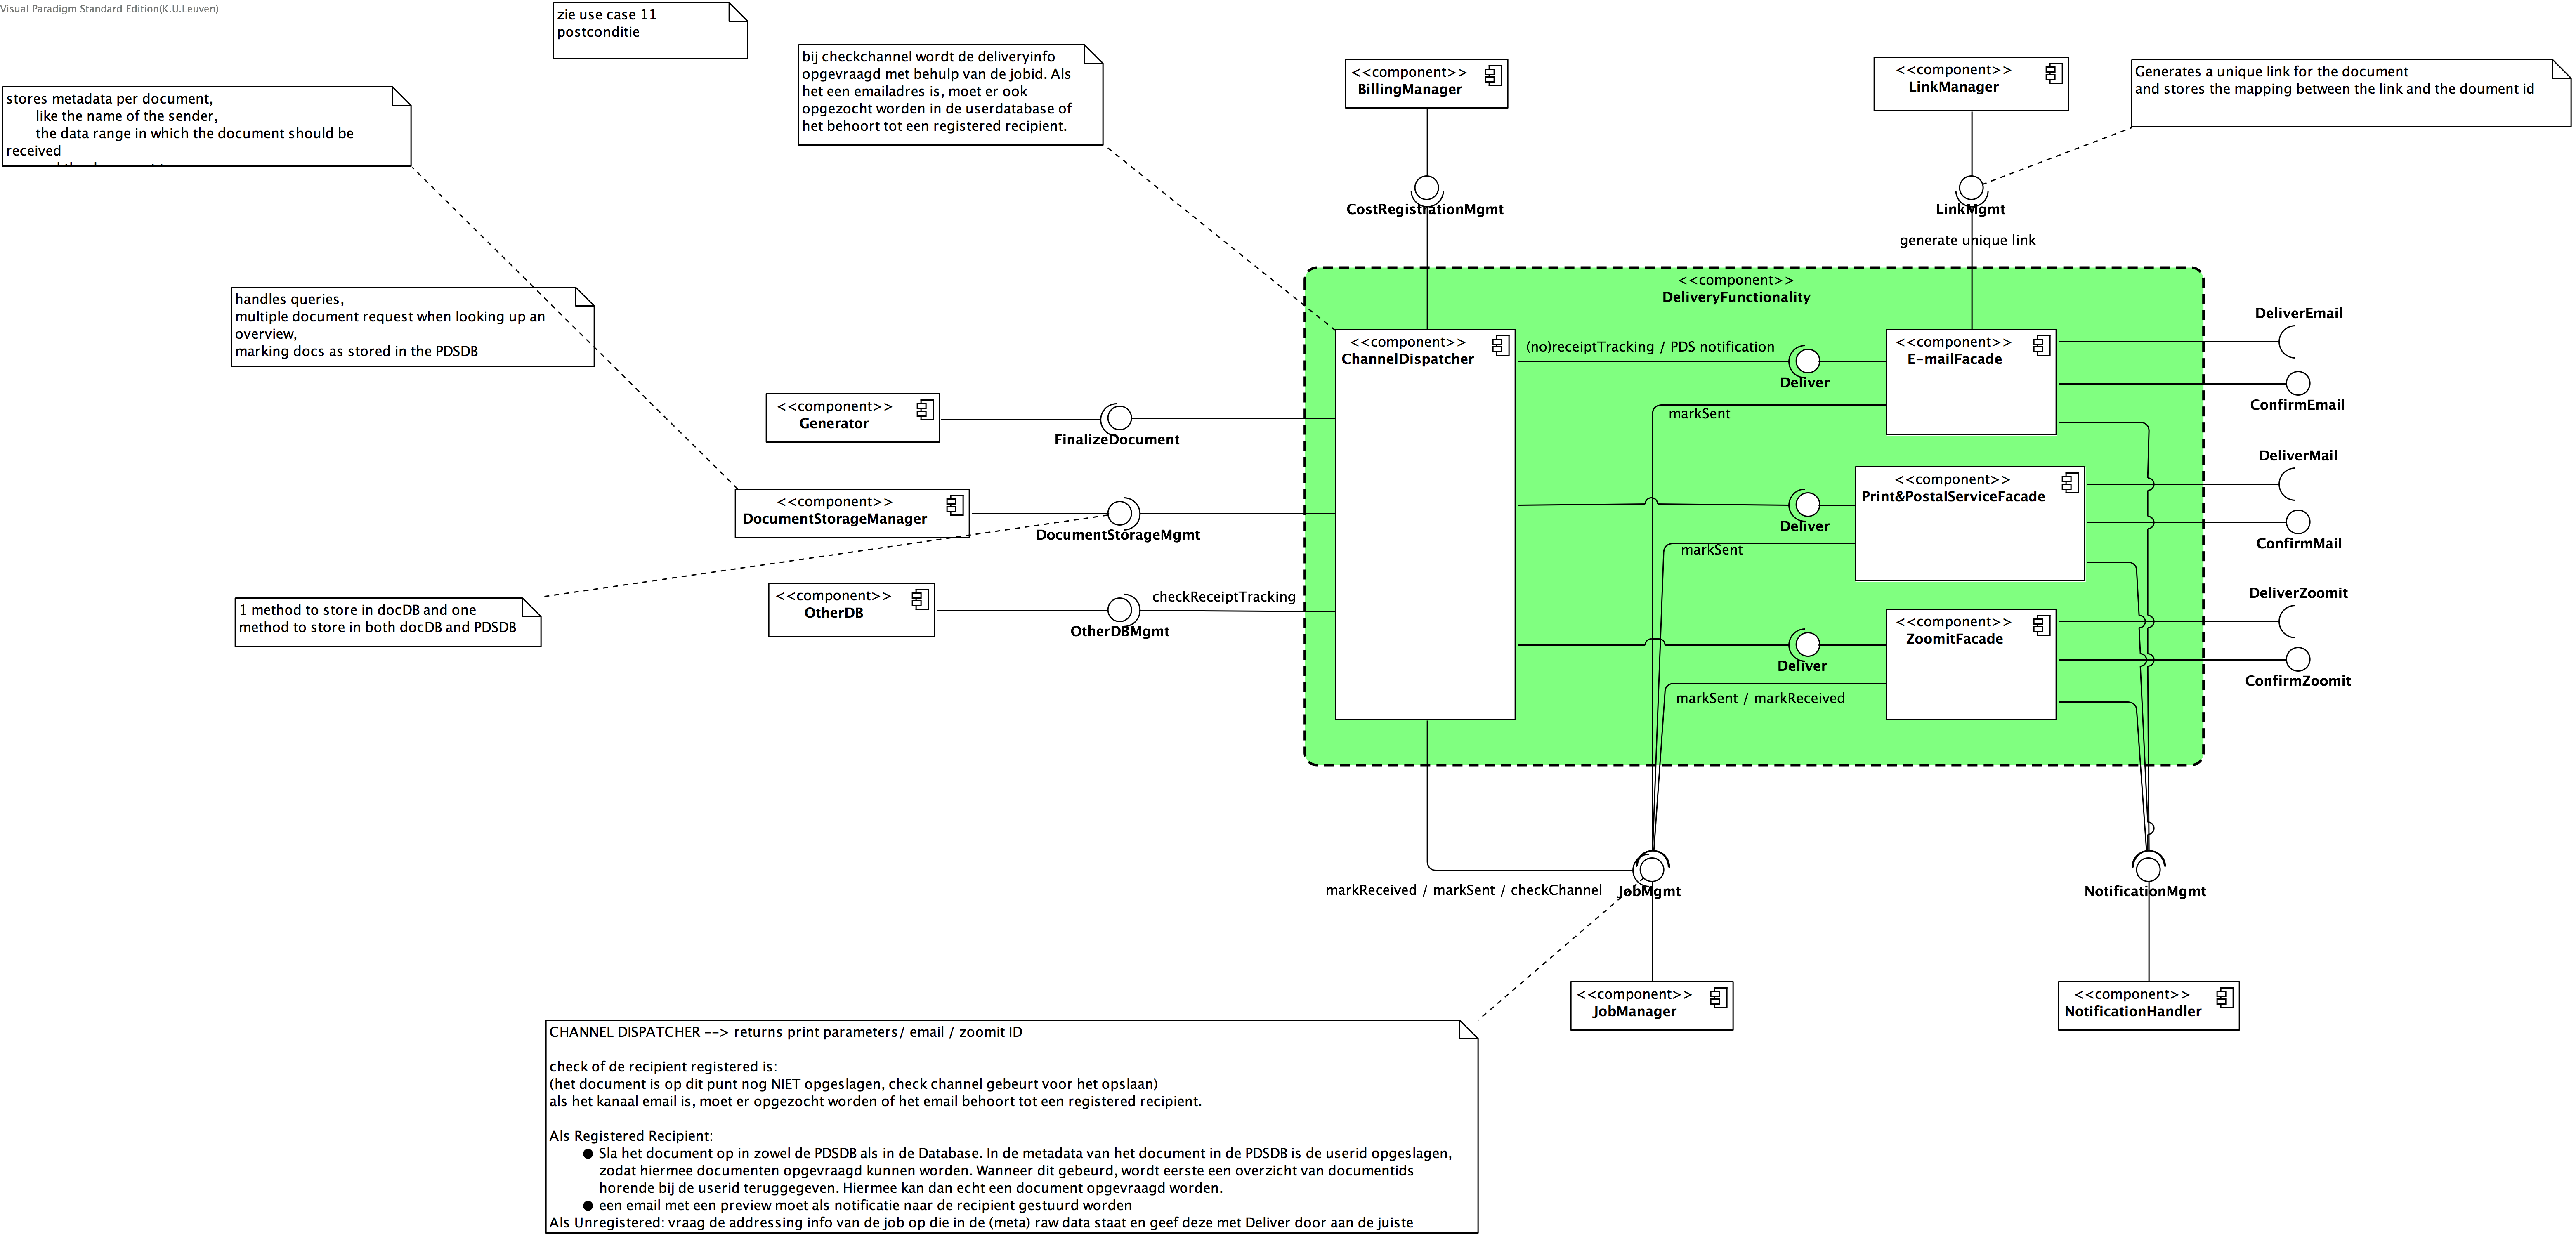
\includegraphics[width=0.8\textwidth]{DeliveryFunctionality.png}
	\caption{Decomposition of \texttt{DeliveryFunctionality}}
	\label{fig:decomp-DeliveryFunctionality}
\end{figure}
\FloatBarrier

Describe the decomposition of \texttt{ComponentX} and how this relates to the
requirements.

\subsection{DocumentDB}\label{subsec:decomp-DocumentDB}
Note that there must also be a (sub)component monitoring all requests to the shards, in order to throttle excessive requests when necessary. Since this is a rather simple task and the (sub)component must be aware of the details concerning the sharding architecture to efficiently fulfil its purpose, this functionality is delegated to the \texttt{ShardingManager} itself. Finally, this \texttt{ShardingManager} is also responsible for implicitly pinging all \texttt{DocumentDBShards} upon reading and writing in them.
\begin{figure}[!htp]
	\centering
	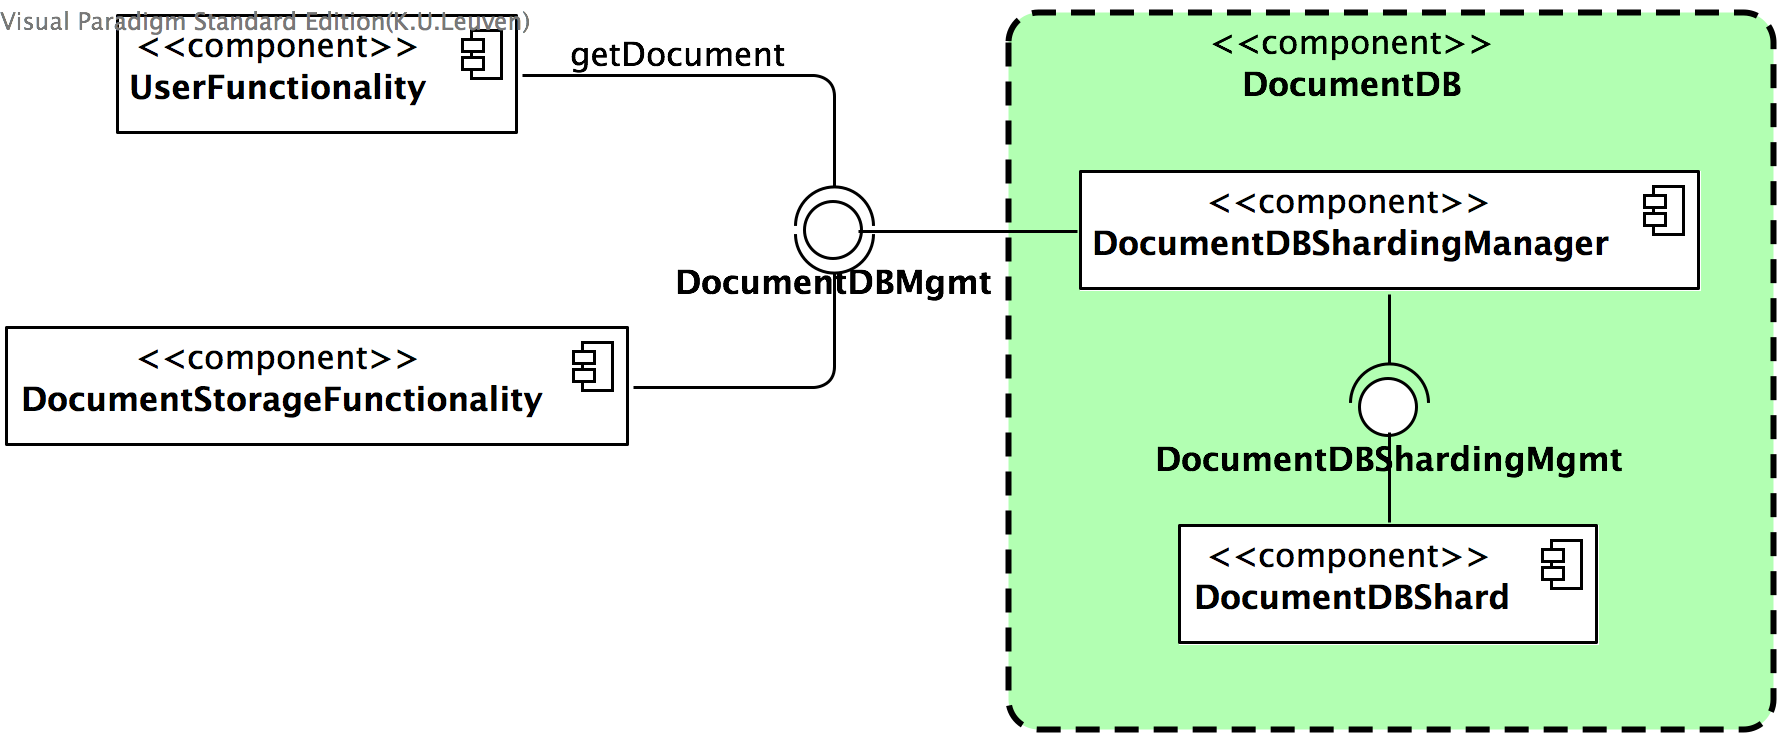
\includegraphics[width=0.8\textwidth]{DocumentDB.png}
	\caption{Decomposition of \texttt{DocumentDB}}
	\label{fig:decomp-DocumentDB}
\end{figure}
\FloatBarrier

\subsection{DocumentGenerationManager}\label{subsec:decomp-DocumentGenerationManager}
\begin{figure}[!htp]
	\centering
	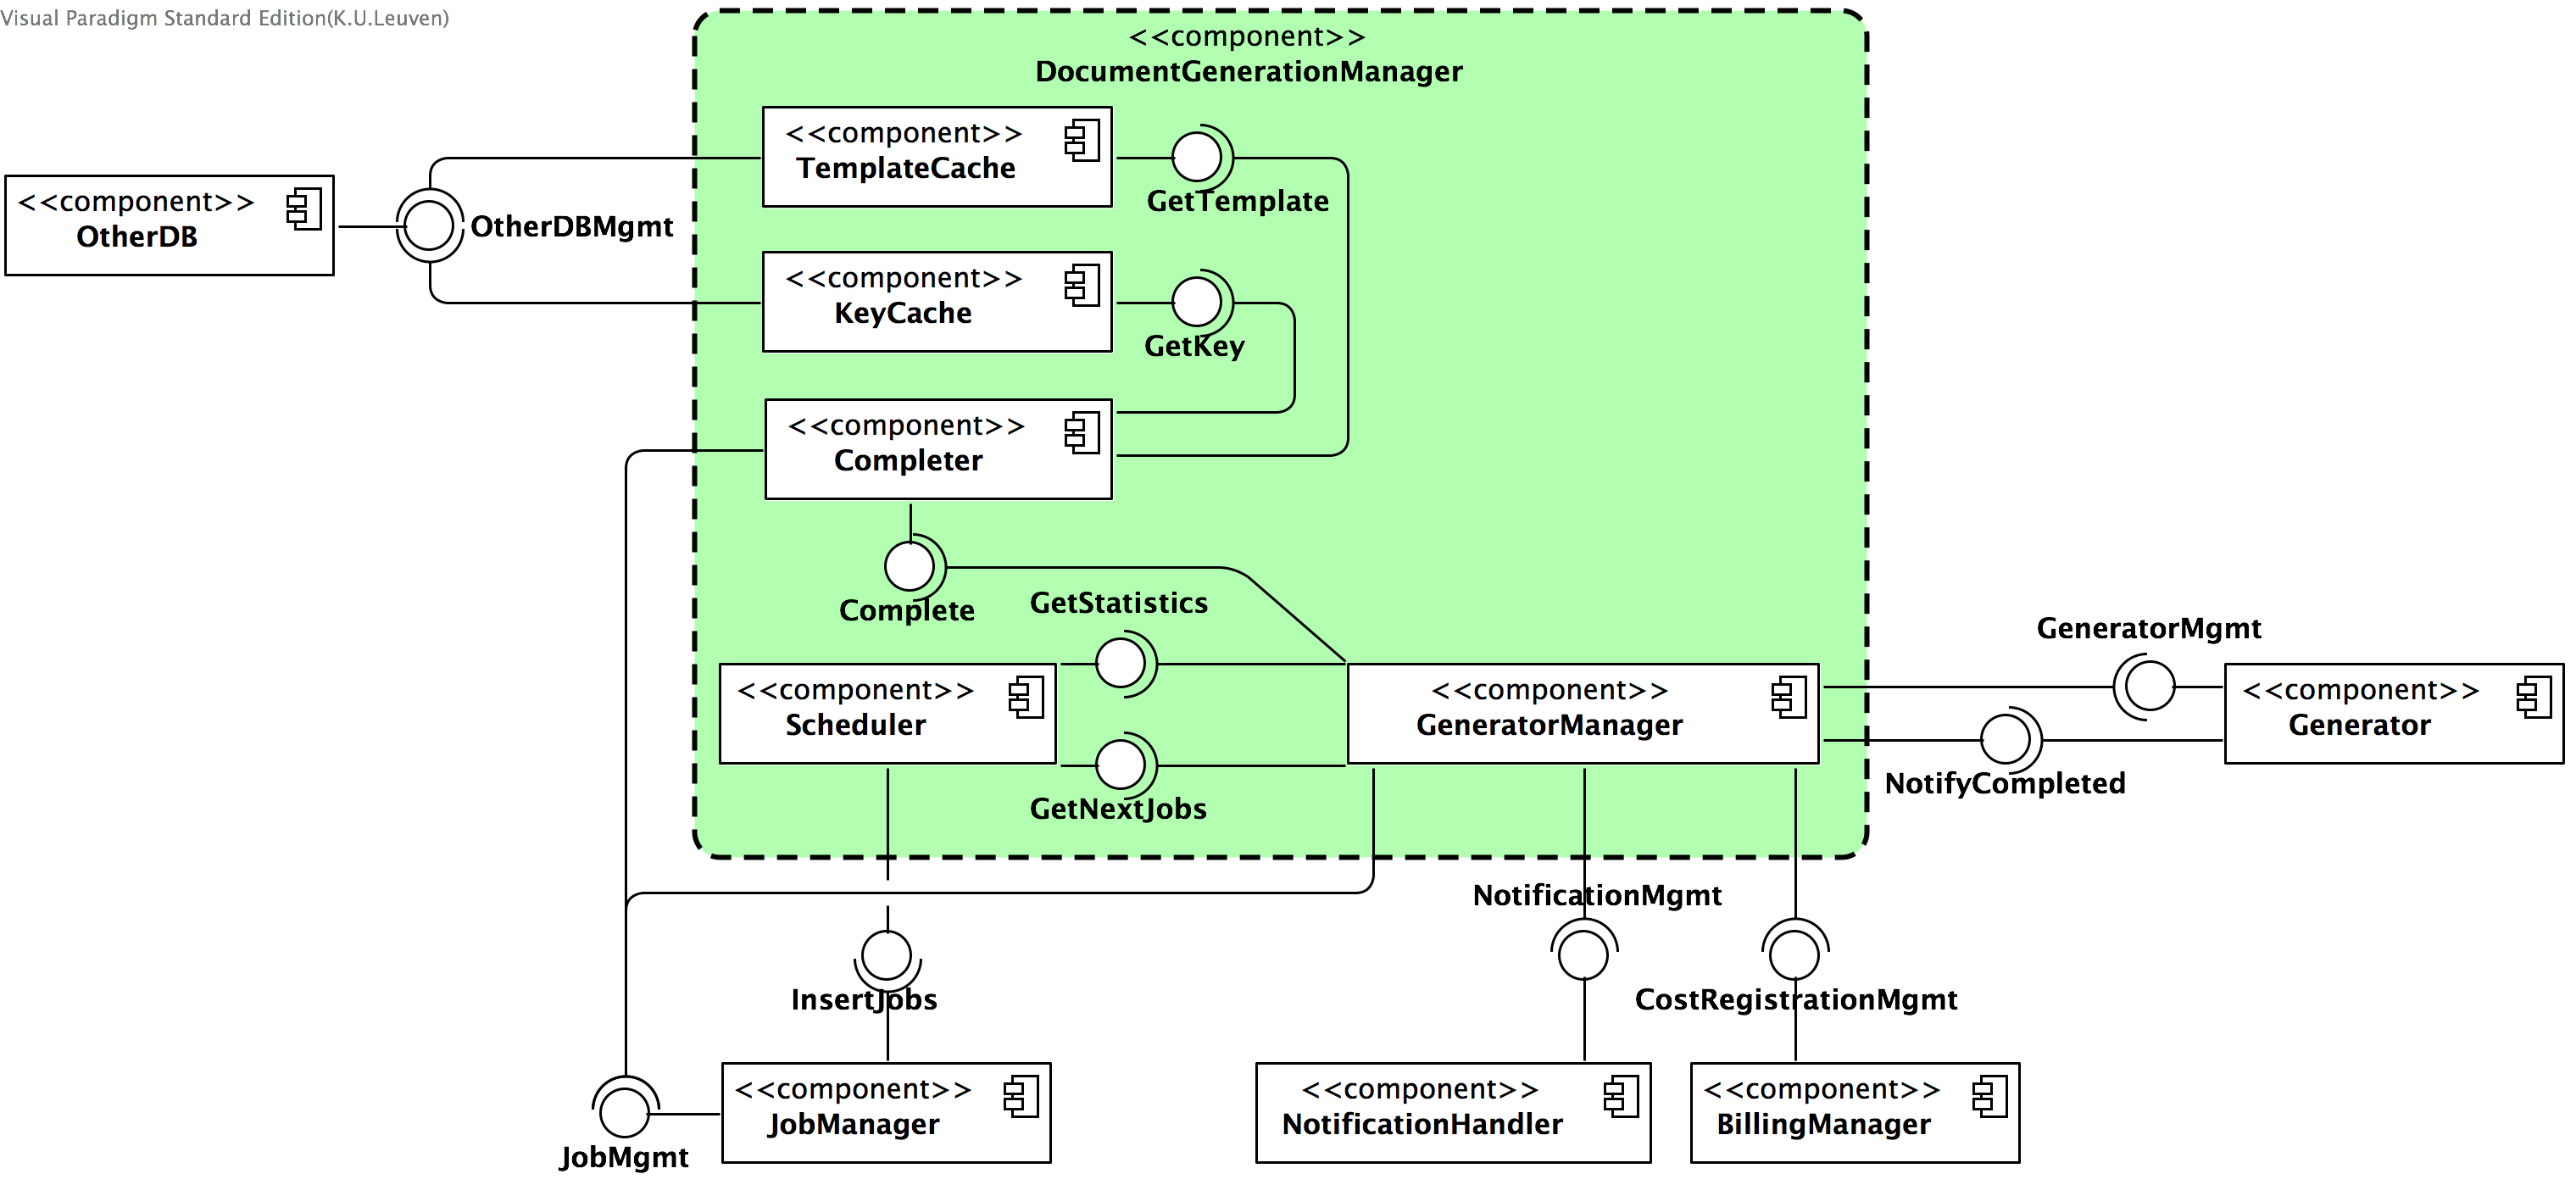
\includegraphics[width=0.8\textwidth]{DocumentGenerationManager.png}
	\caption{Decomposition of \texttt{DocumentGenerationManager}}
	\label{fig:decomp-DocumentGenerationManager}
\end{figure}
\FloatBarrier

\subsection{DocumentStorageFunctionality}\label{subsec:decomp-DocumentStorageFunctionality}
The storage of documents is handled by the \texttt{DocumentStorageManager}, which receives generated documents from the intermediary \texttt{OtherFunctionality2} component and stores them in either the \texttt{DocumentDB} (for unregistered recipients) or in both the \texttt{DocumentDB} and the \texttt{PDSDB} (for registered recipients) according to the method that is invoked on it. The necessity for this component follows from the fact that synchronisation is needed between the two storage components mentioned above. Note that the PDSDocMgmt interface in the \texttt{PDSDB} component now requires an extra method to save documents.
\begin{figure}[!htp]
	\centering
	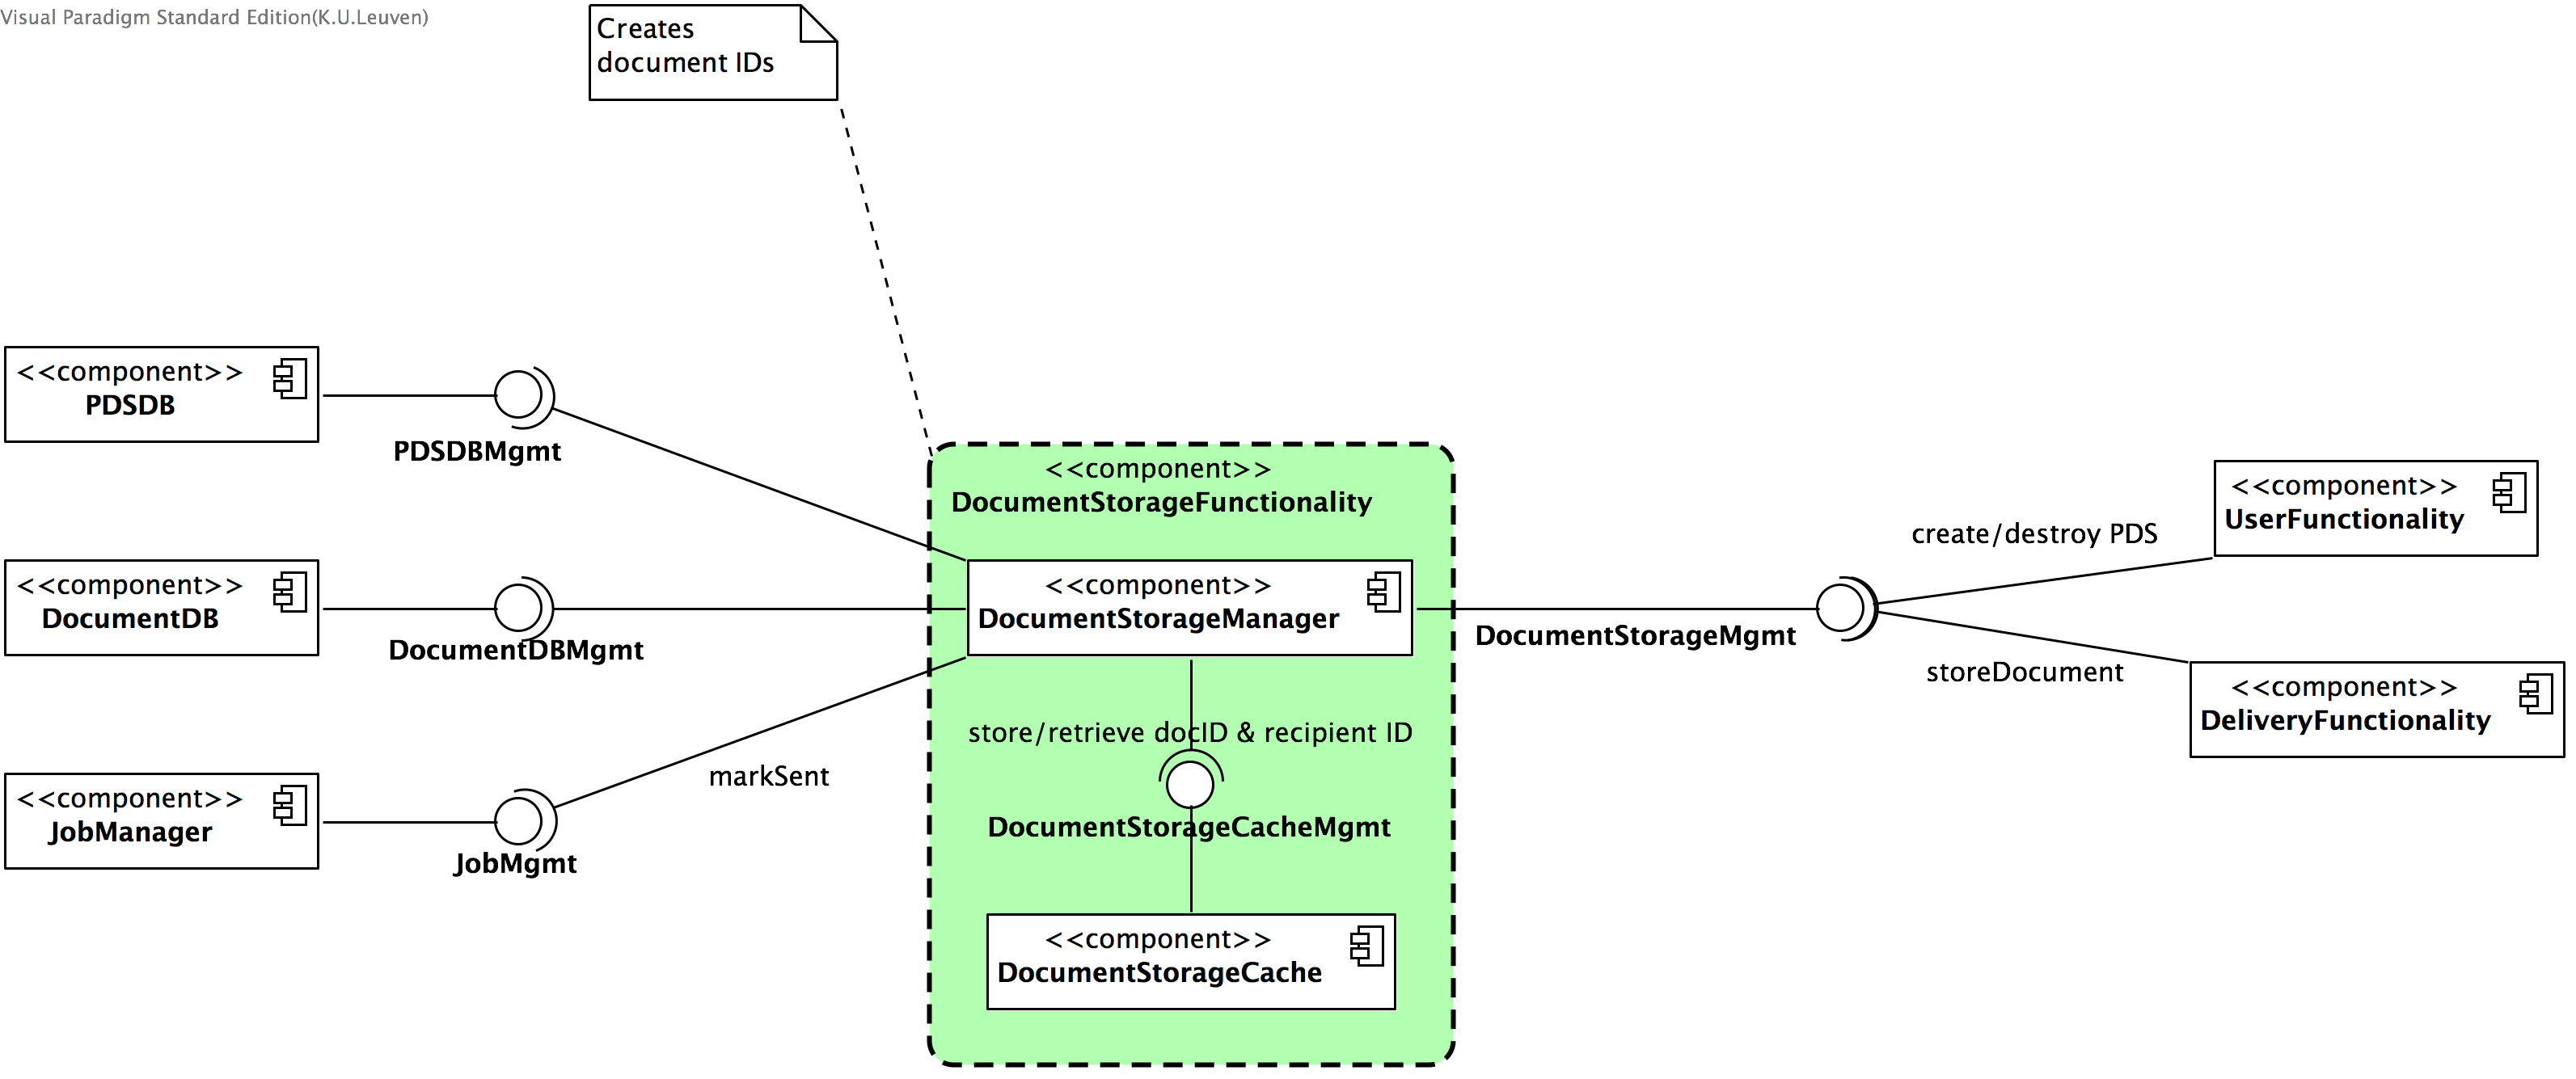
\includegraphics[width=0.8\textwidth]{DocumentStorageFunctionality.png}
	\caption{Decomposition of \texttt{DocumentStorageFunctionality}}
	\label{fig:decomp-DocumentStorageFunctionality}
\end{figure}
\FloatBarrier

\subsection{JobManager}\label{subsec:decomp-JobManager}
\begin{figure}[!htp]
	\centering
	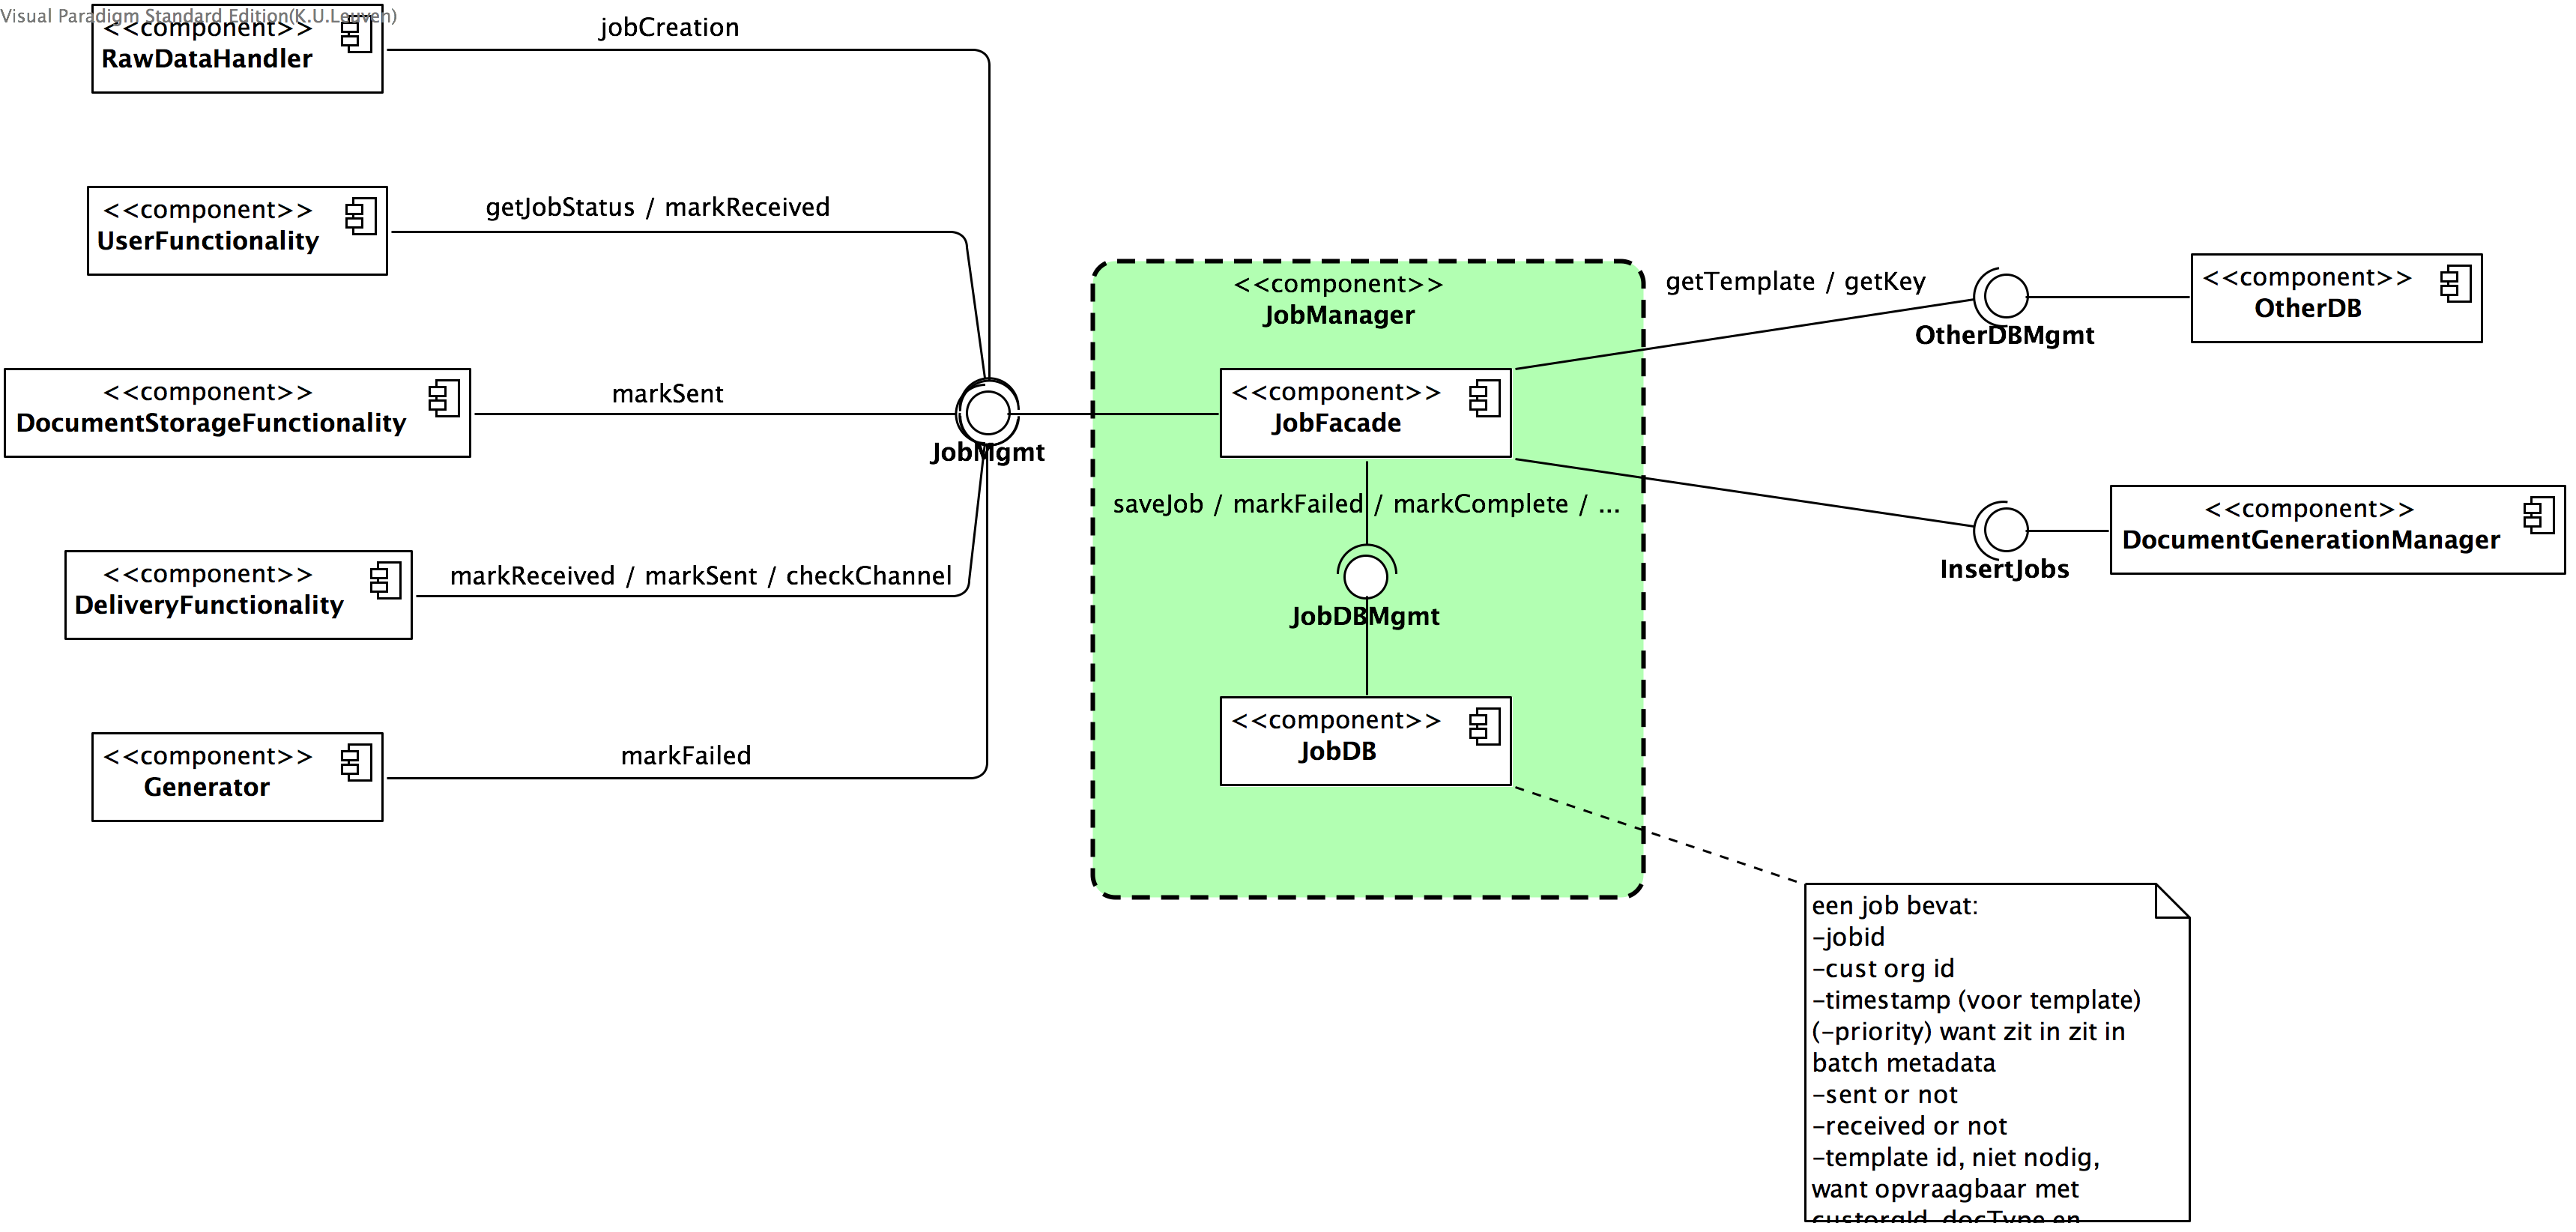
\includegraphics[width=0.8\textwidth]{JobManager.png}
	\caption{Decomposition of \texttt{JobManager}}
	\label{fig:decomp-JobManager}
\end{figure}
\FloatBarrier

\subsection{LinkMappingFunctionality}\label{subsec:decomp-LinkMappingFunctionality}
Motivatie voor LinkManager: Checks expiration date ALS DAT NODIG IS--> reason: links naar de pdsdb vervallen niet (zolang de gebruik geregistreerd is)
LinkManager maps link to (document ID, place where the document is stored)-pairs --> REASON: the unique link has two possible sources: an e-mail to an unregistered recipient or an email to a registered recipient. For an unregistered recipient, the RecipientFacade must look with the documentid for the document in the documentDB. For a registered recipient, the RecipientFacade must look with the documentid for the document  in the PDSDB. (Mogelijk een boolean ofzo)
Does NOT do mapping removal after x years --> there has to be a notification when the link has expired
\begin{figure}[!htp]
	\centering
	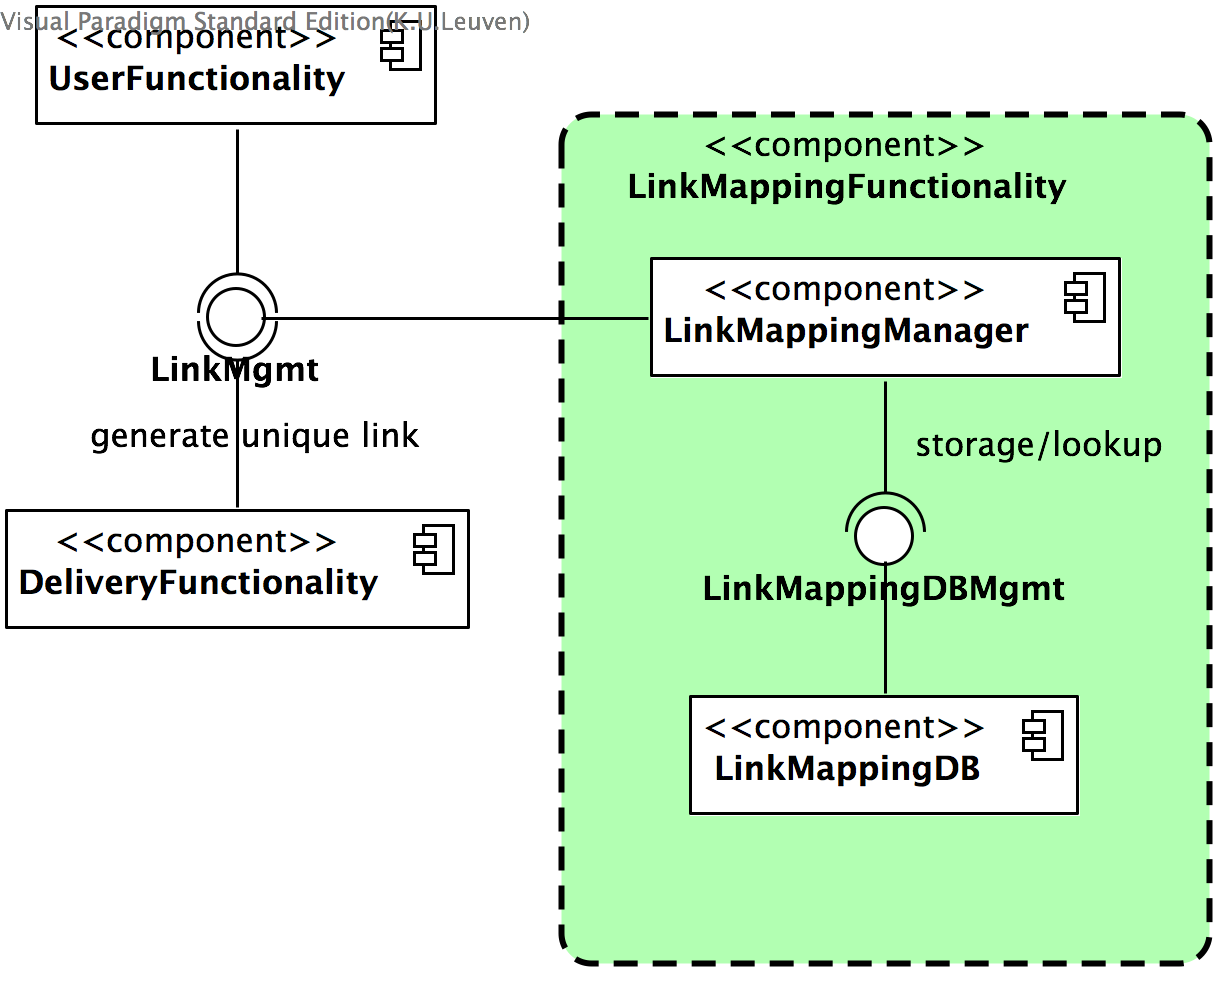
\includegraphics[width=0.8\textwidth]{LinkMappingFunctionality.png}
	\caption{Decomposition of \texttt{LinkMappingFunctionality}}
	\label{fig:decomp-LinkMappingFunctionality}
\end{figure}
\FloatBarrier

\subsection{PDSDB}\label{subsec:decomp-PDSDB}
\begin{figure}[!htp]
	\centering
	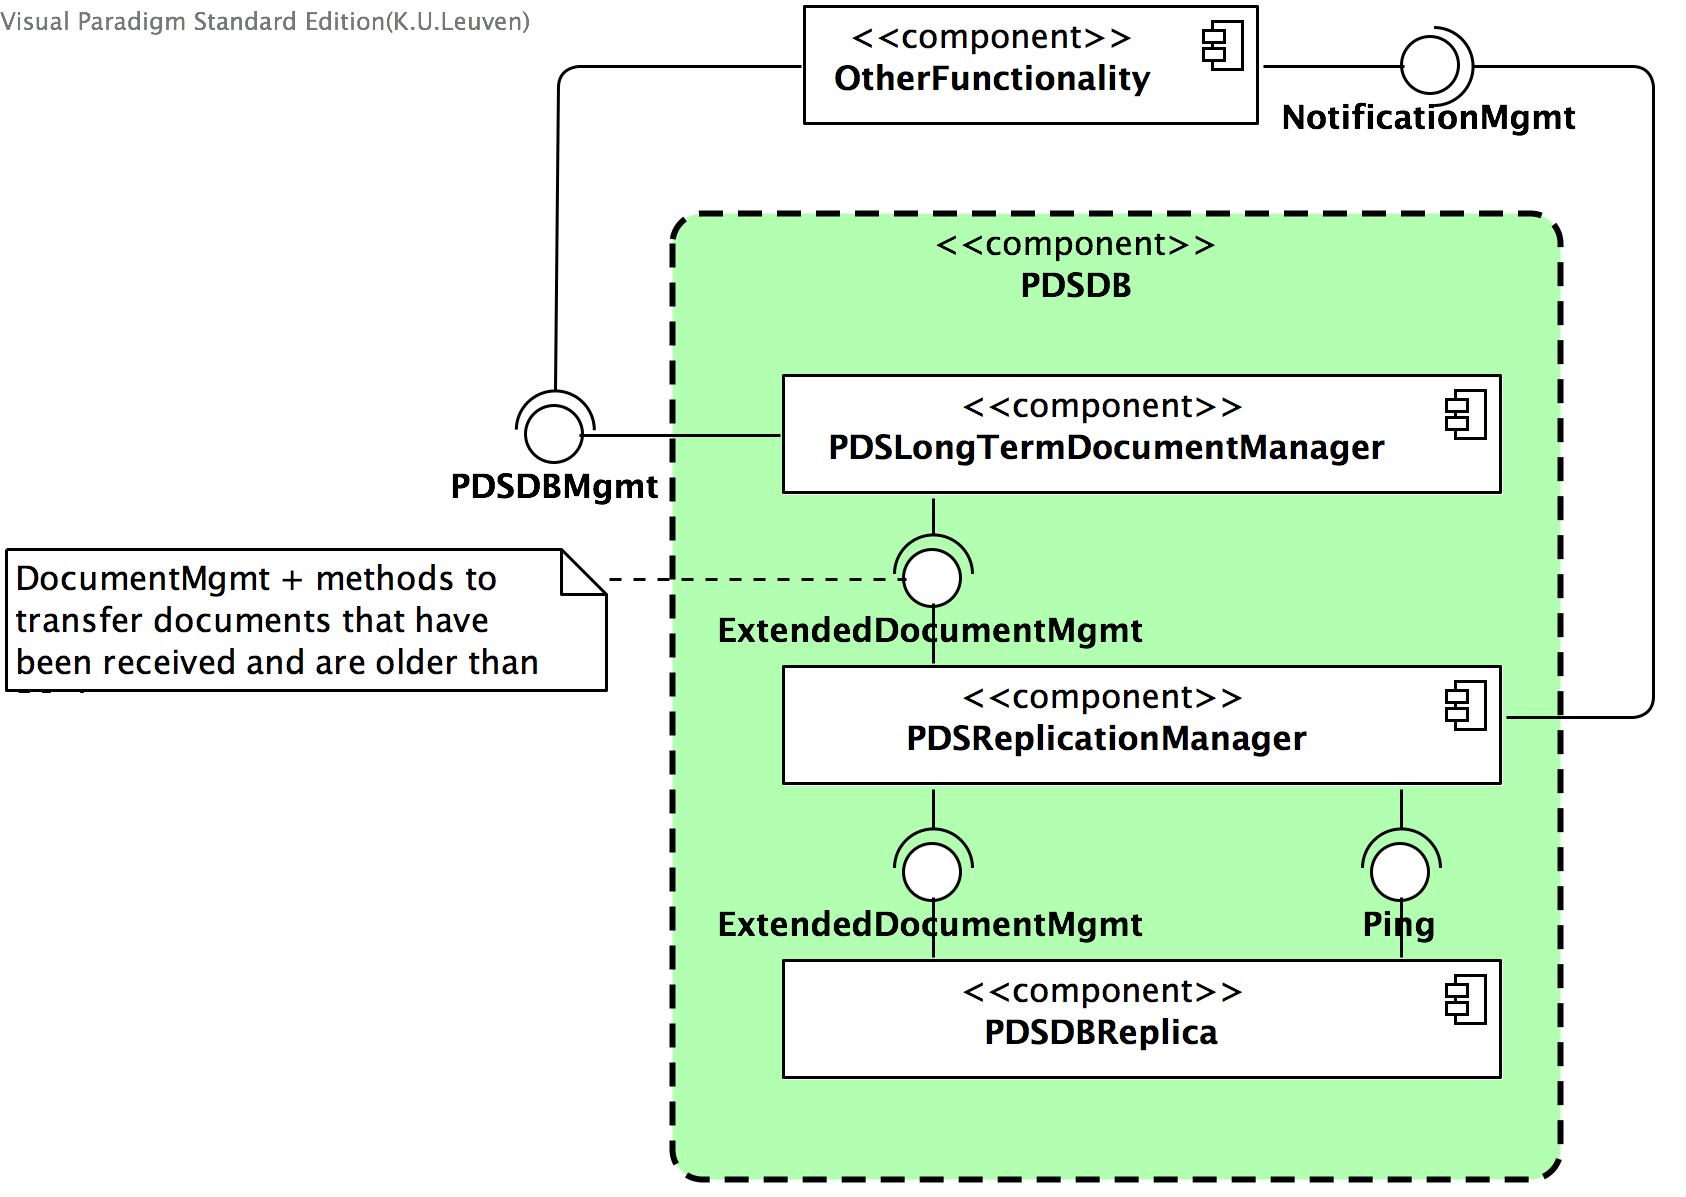
\includegraphics[width=0.8\textwidth]{PDSDB.png}
	\caption{Decomposition of \texttt{PDSDB}}
	\label{fig:decomp-PDSDB}
\end{figure}
\FloatBarrier

\subsection{UserFunctionality}\label{subsec:decomp-UserFunctionality}
\begin{figure}[!htp]
	\centering
	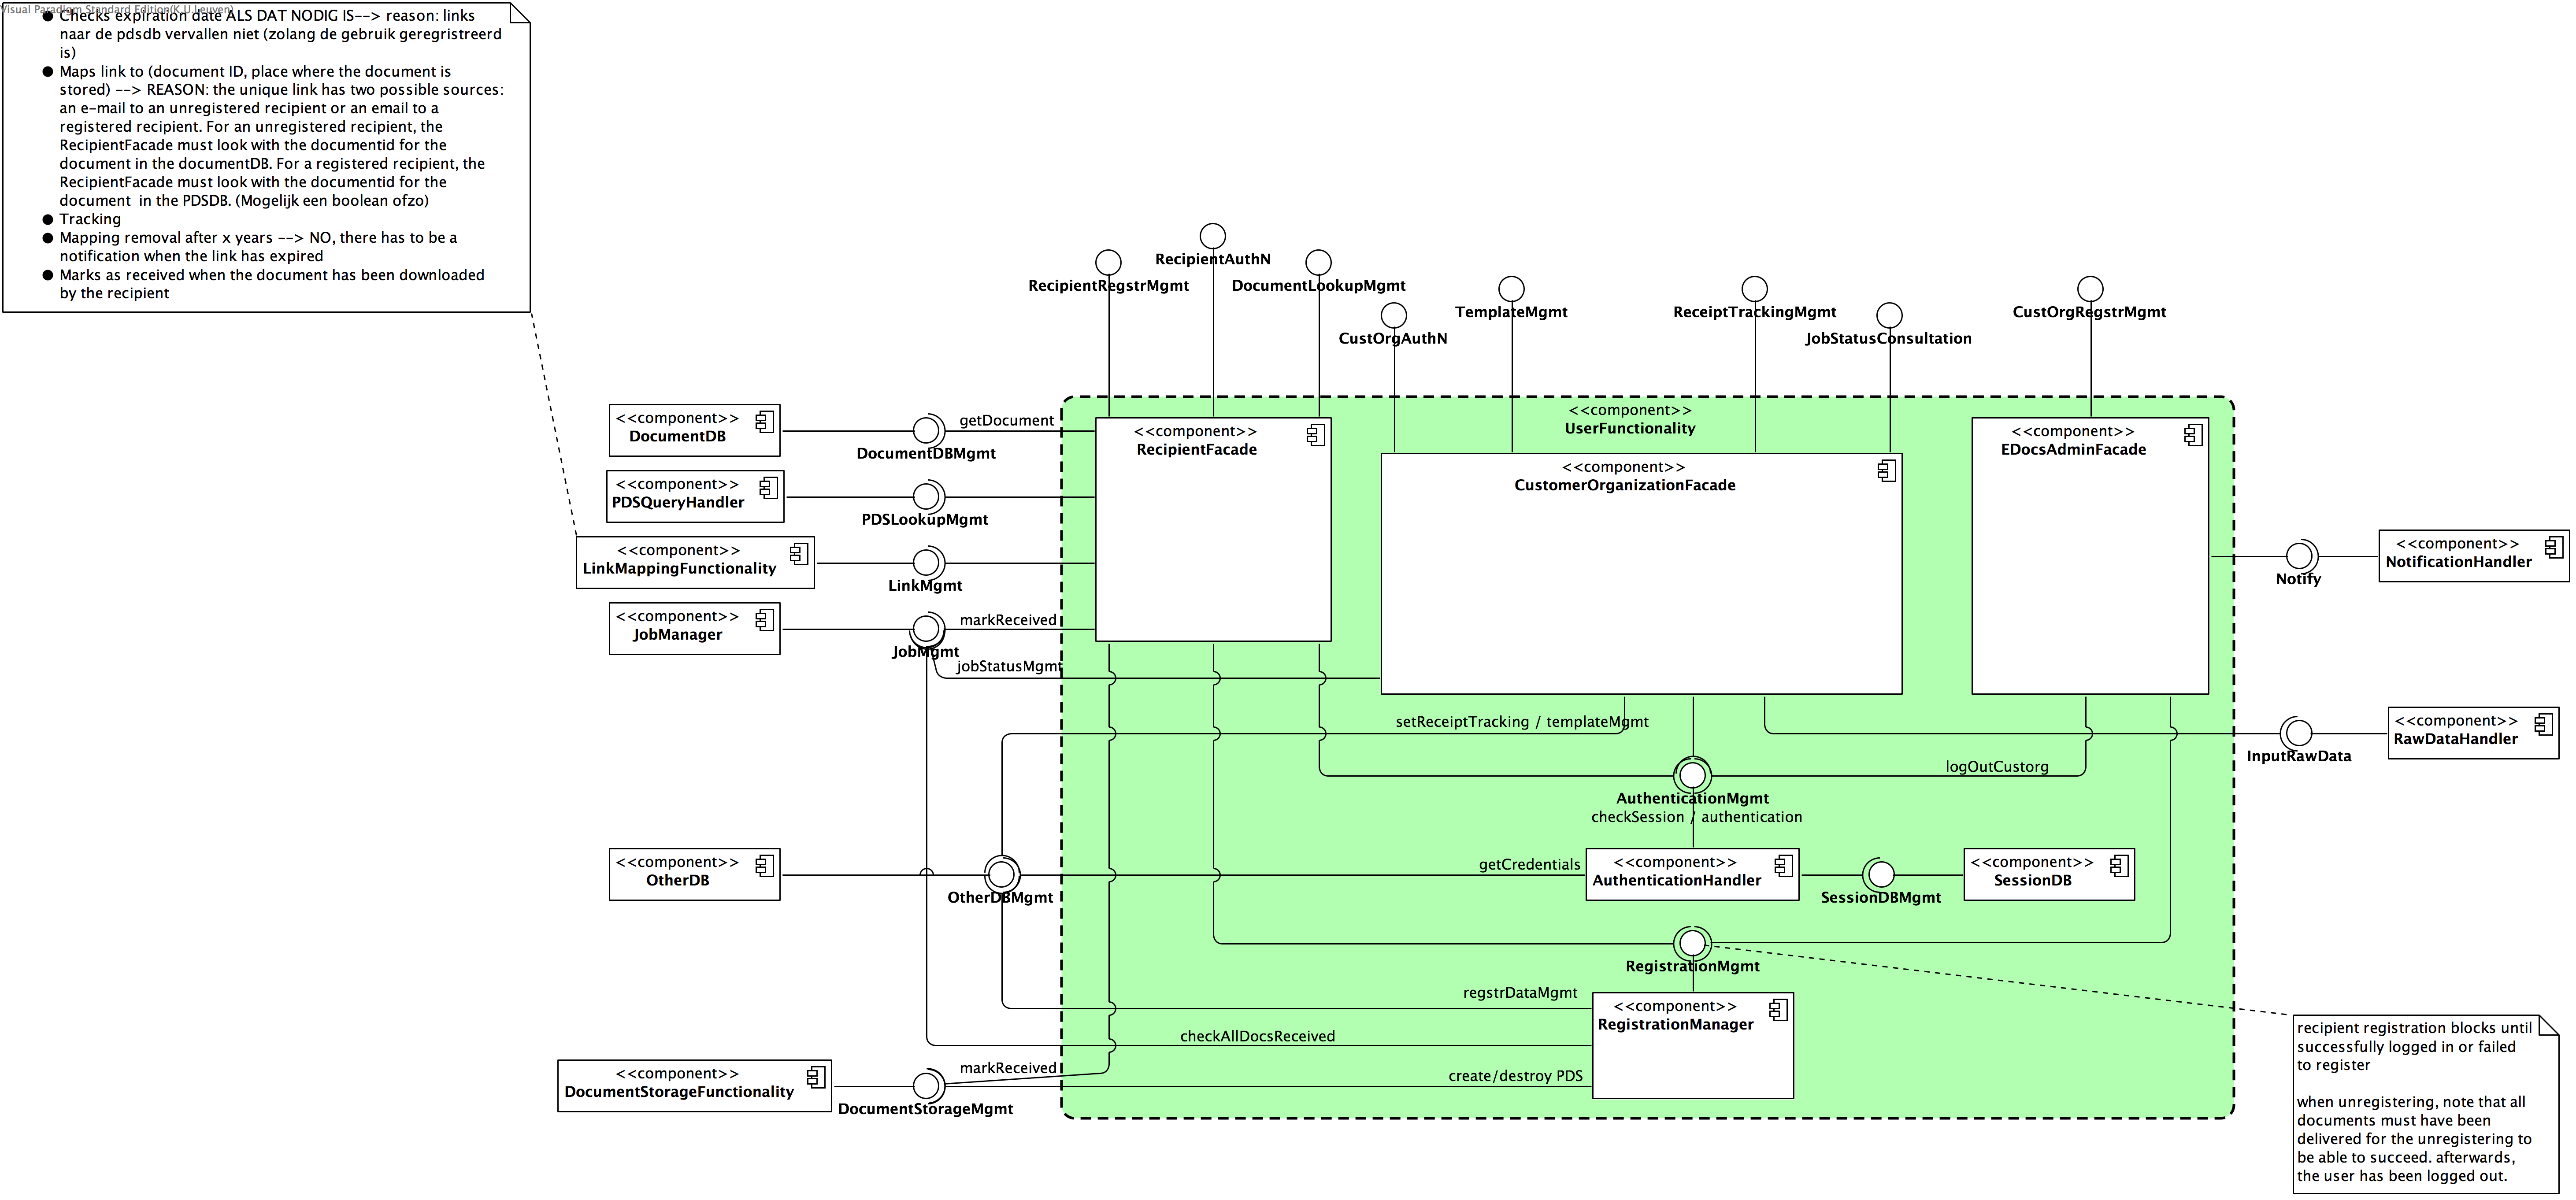
\includegraphics[width=0.8\textwidth]{UserFunctionality.png}
	\caption{Decomposition of \texttt{UserFunctionality}}
	\label{fig:decomp-UserFunctionality}
\end{figure}
\FloatBarrier

\section{Deployment view (UML Deployment diagram)}\label{sec:deployment}
Describe the context diagram for the deployment view.
For example, which protocols are used for communication with external systems
and why?

\begin{figure}[!htp]
	\centering
	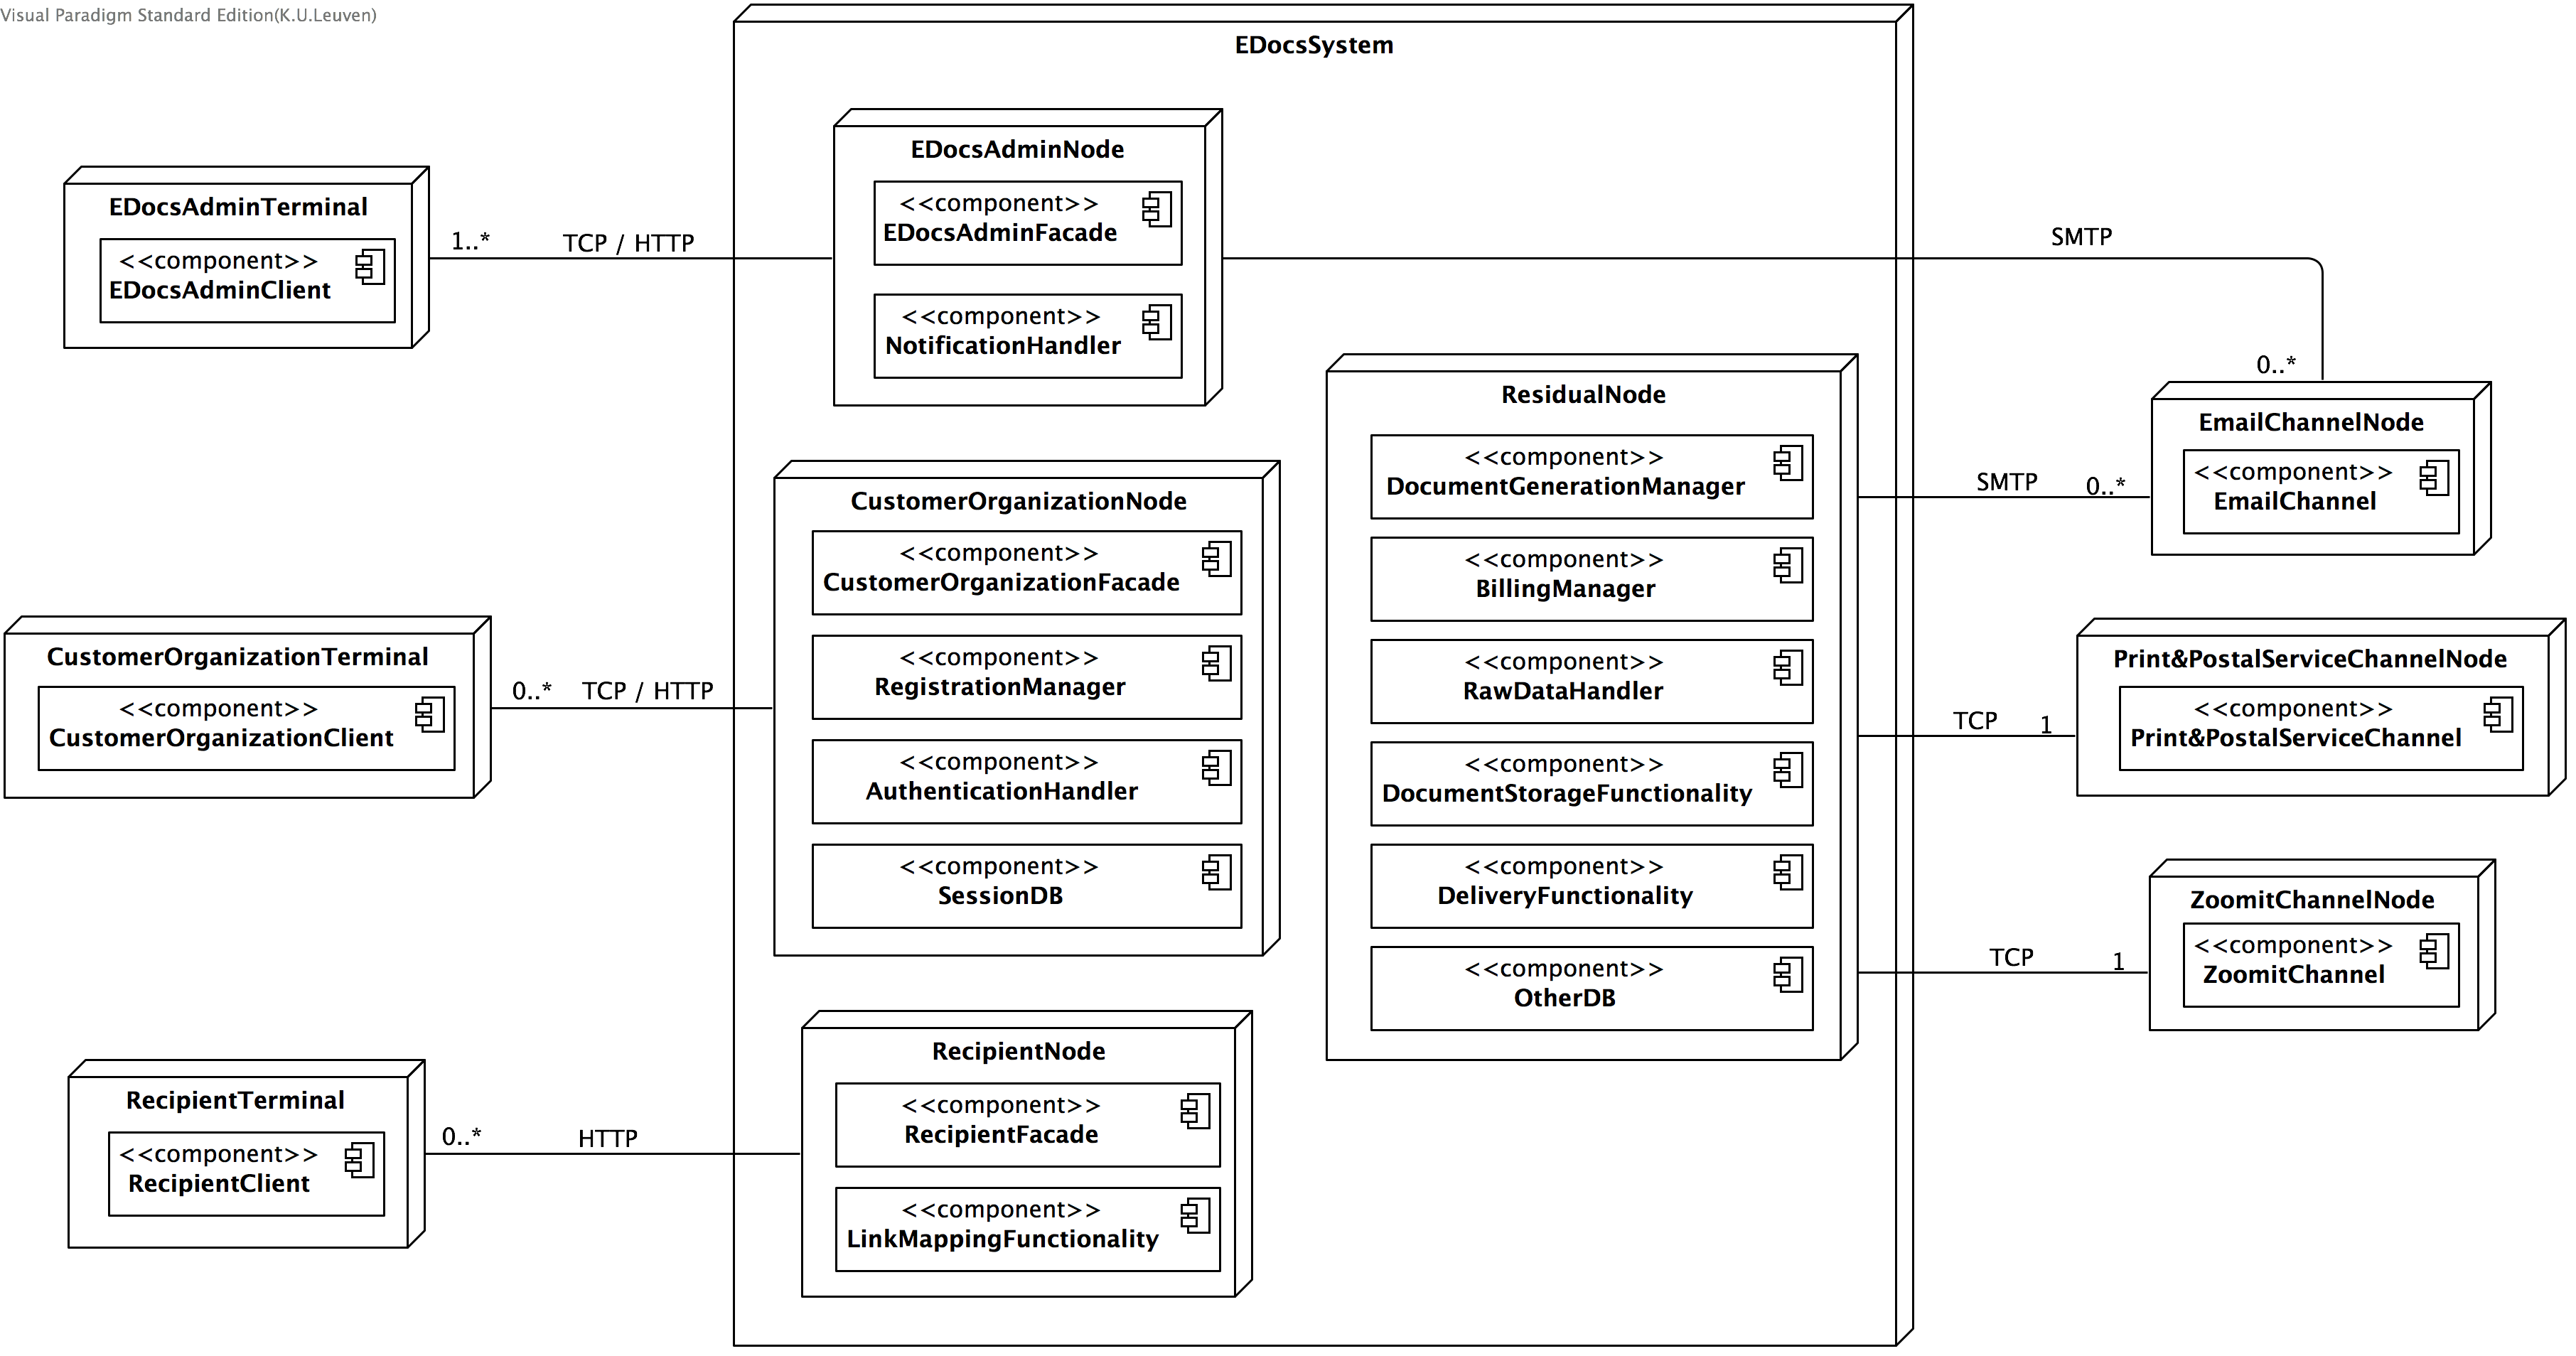
\includegraphics[width=0.8\textwidth]{ContextDeployment.png}
    \caption{Context diagram for the deployment view.}
    \label{fig:depl_context}
\end{figure}
\FloatBarrier

The primary deployment diagram itself and accompanying explanation.
Pay attention to the parts of the deployment diagram which are crucial for
achieving certain non-functional requirements.
Also discuss any alternative deployments that you considered.

\begin{figure}[!htp]
    \centering
	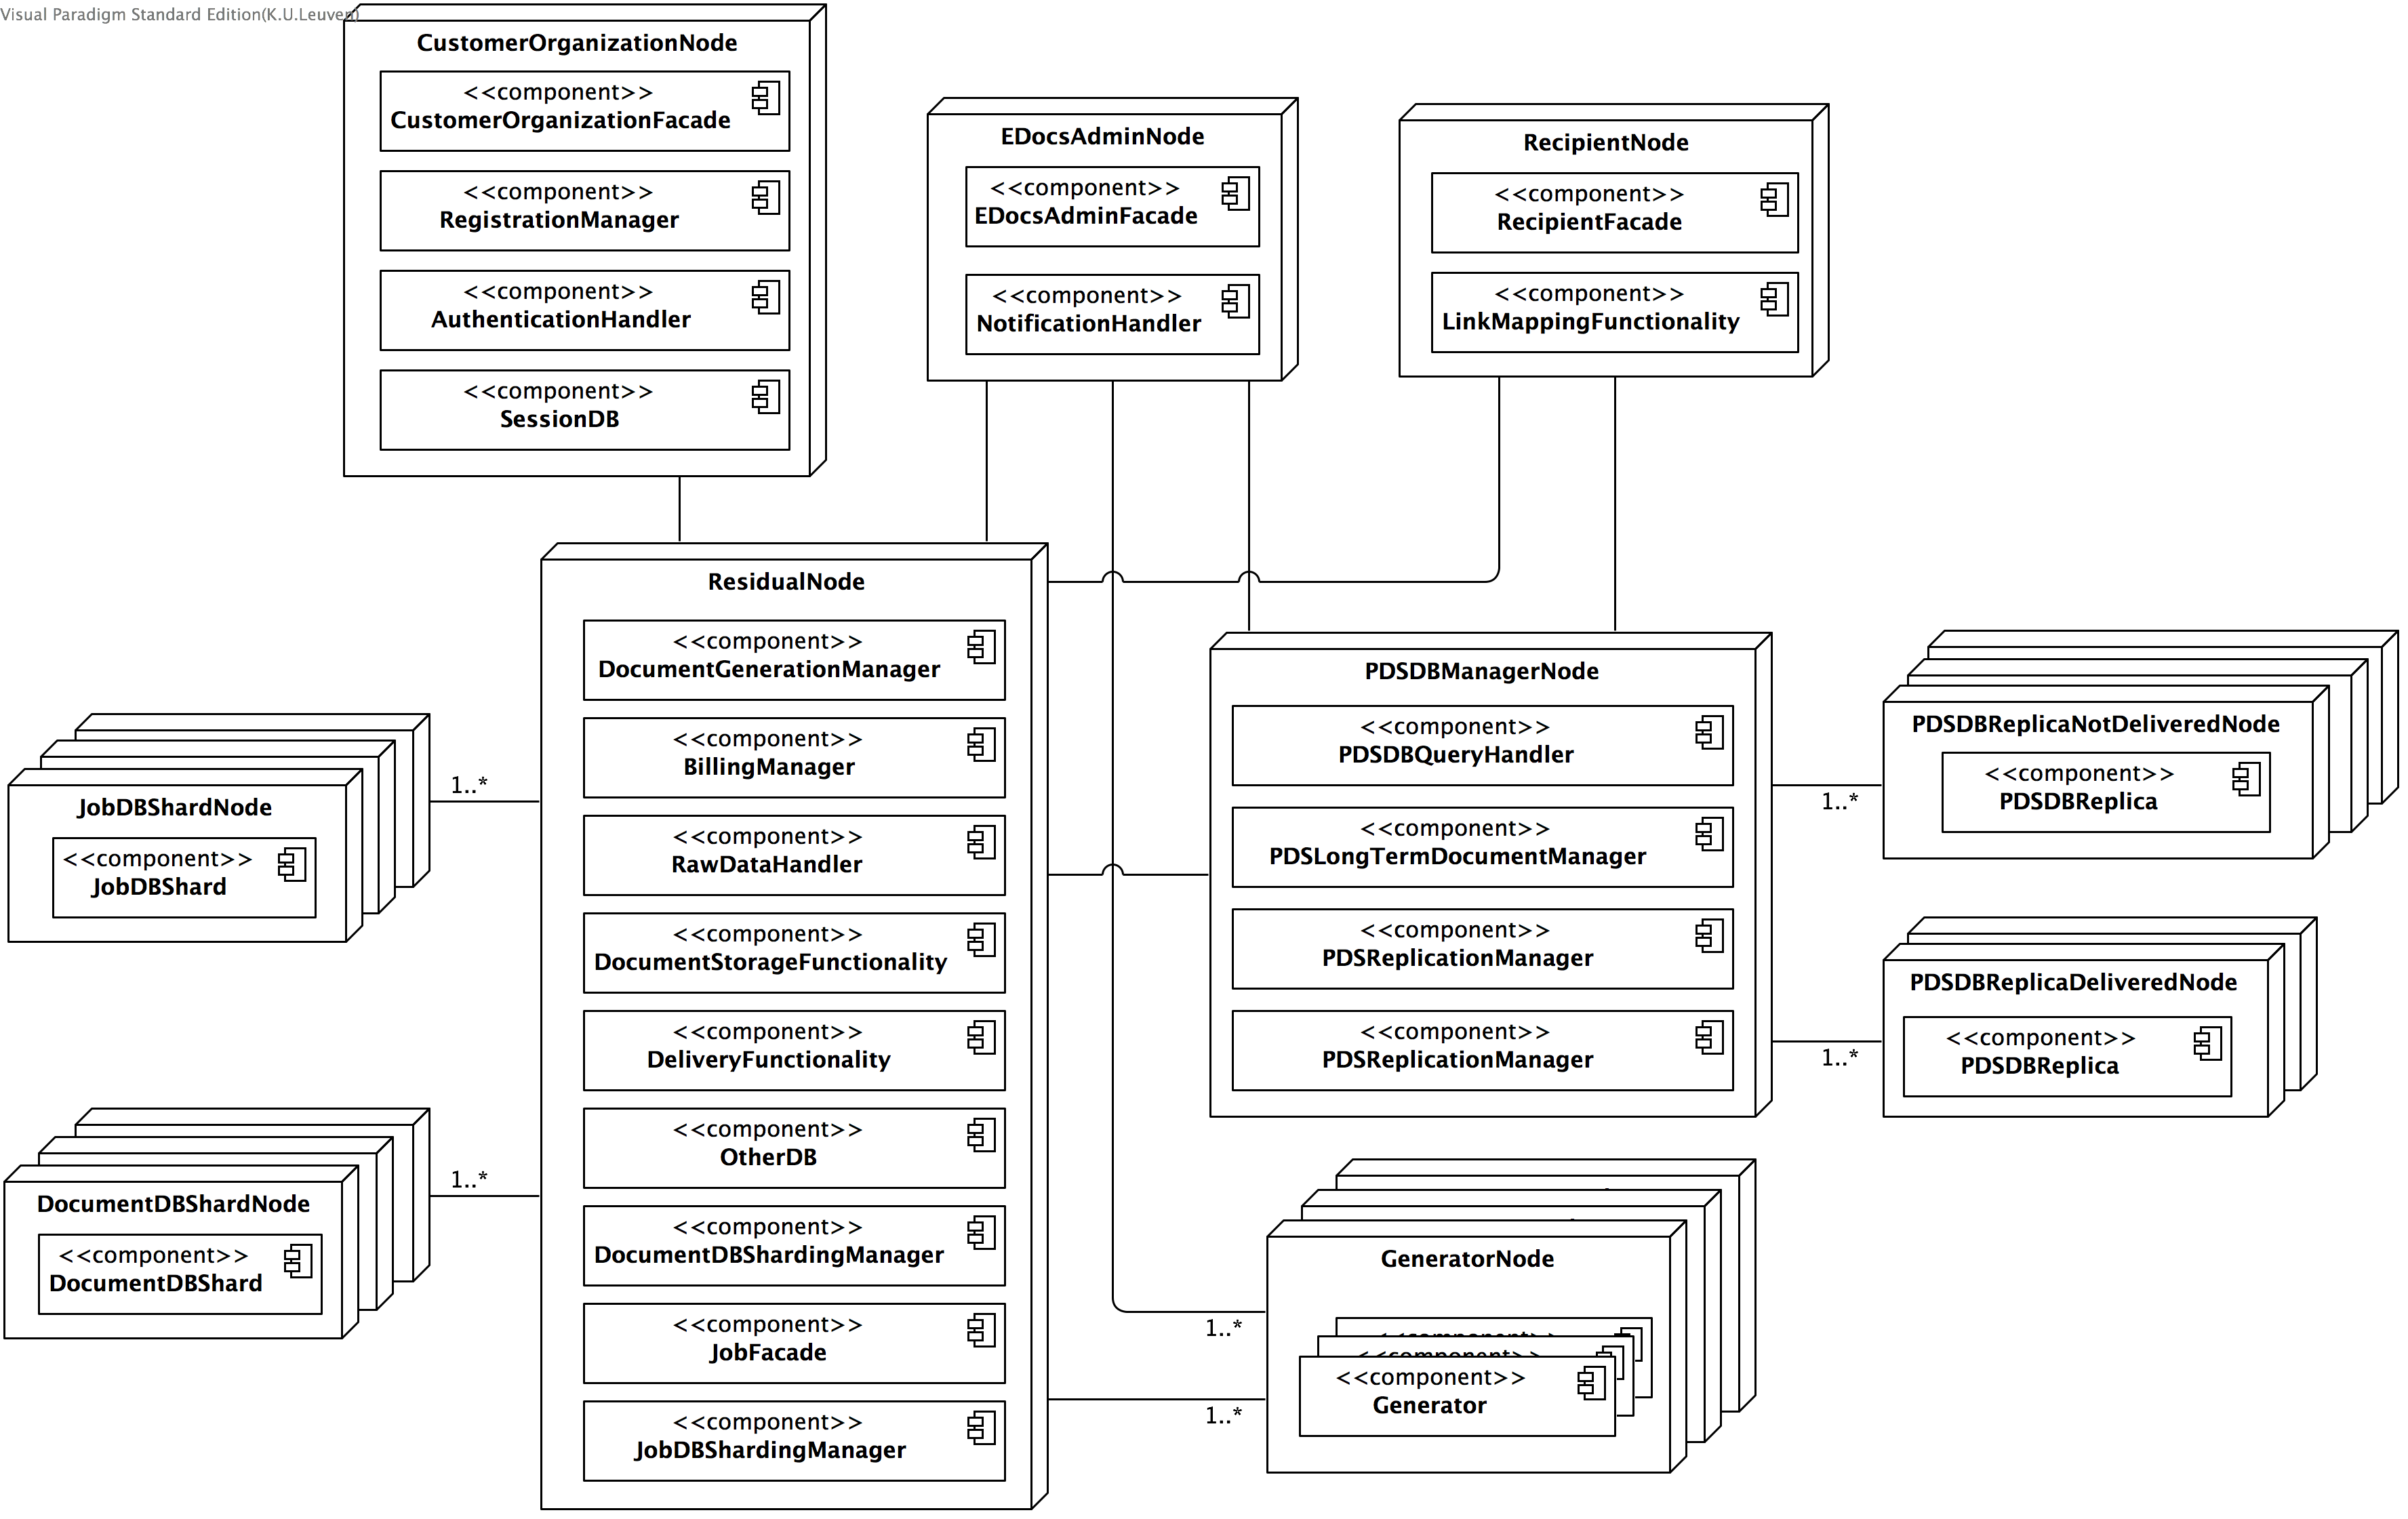
\includegraphics[width=0.8\textwidth]{TotalDeployment.png}
    \caption{Primary diagram for the deployment view.}
    \label{fig:depl_primary}
\end{figure}
\FloatBarrier

\section{Scenarios}\label{sec:scenarios}
Illustrate how your architecture fulfills the most important data flows.
As a rule of thumb, focus on the scenario of the domain description.
Describe the scenario in terms of architectural components using UML Sequence
diagrams and further explain the most important interactions in text.
Illustrating the scenarios serves as a quick validation of the completeness of
your architecture.
If you notice at this point that for some reason, certain functionality or
qualities are not addressed sufficiently in your architecture, it suffices to
document this, together with a rationale of why this is the case according to
you.
You do not have to further refine you architecture at this point.

\subsection{Scenario 1}
Shortly describe the scenario shown in this subsection.
Show the complete scenario using one or more sequence diagrams.

\begin{figure}[!htp]
    \centering
    %\includegraphics[width=\textwidth]{}
    \missingfigure[figwidth=0.8\textwidth]{Sequence diagram scenario 1}
    \caption{The system behavior for the first scenario.
        }\label{fig:seq_scenario1}
\end{figure}


\subsection{A registered recipient logs in}
Figure \ref{fig:seq_UC1LogIn} depicts the sequence diagram of a Registered Recipient logging in, according to \emph{UC1: Log in}. The Registered Recipient provides his details to the \texttt{RecipientFacade}. The \texttt{Authentication} compares these credentials to those stored in the \texttt{OtherDB}. if the given credentials match the stored credentials, a new session is opened in the \texttt{SessionDB} and the corresponding session identifier is returned to the registered recipient. Otherwise, an InvalidCredentialsException is thrown.\\
Note that the use case \emph{UC1: Log in} also has the Customer Organization as a primary actor. The login procedure for customer organizations is almost identical to the procedure for registered recipient, which is why we do not provide a separate sequence diagram for this primary actor. Compared to figure \ref{fig:seq_UC1LogIn}, the Customer Organization sends it login request to the \texttt{CustomerOrganizationFacade} instead of the \texttt{RecipientFacade}. Also, another method call to \texttt{OtherDB} is used to ask for the credentials of a customer organization.
\begin{figure}[!htp]
    \centering
    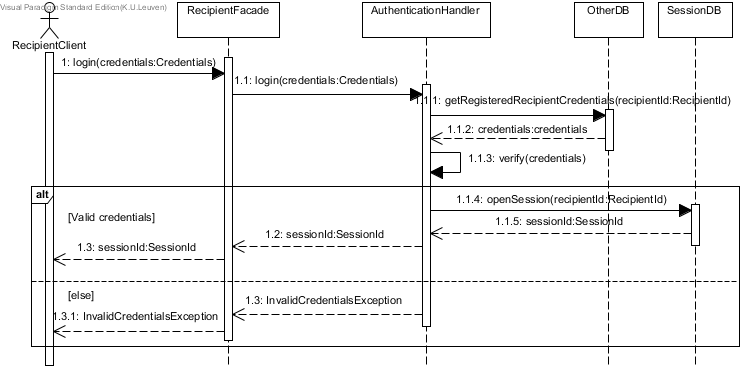
\includegraphics[width=\textwidth]{Seq_UC1LogIn.png}
    \caption{The login behaviour of a Registered Recipient.
        }\label{fig:seq_UC1LogIn}
\end{figure}

\subsection{A registered recipient logs out}
Figure \ref{fig:seq_UC2LogOut} shows the behaviour of a Registered Recipient logging out, according to \emph{UC2: Log out}. The Registered Recipient provides his recipient id and session id to the \texttt{RecipienntFacade}. The \texttt{AuthenticationHandler} first verifies the session (figure \ref{fig:seq_UC2LogOut}). If the session is valid, it logs out the Registered Recipient.\\ Note that the logout procedure for Customer Organizations is almost the same. The only difference is that the Customer Organization sends his logout request to the \texttt{CustomerOrganizationFacade} instead of the \texttt{RecipientFacade}. Because of this reason, we do not give a separate sequence diagram for the Customer Organization logging out.

\begin{figure}[!htp]
    \centering
    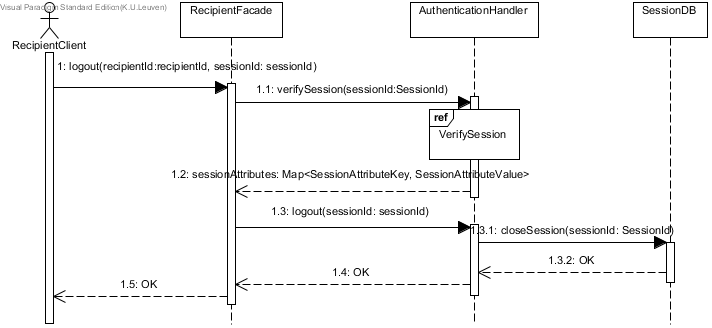
\includegraphics[width=\textwidth]{Seq_UC2LogOut.png}
    \caption{The logout behaviour of the Registered Recipient.
        }\label{fig:seq_UC2LogOut}
\end{figure}



\subsection{Updating a document template}
Figure \ref{fig:seq_UC20UpdateDocumentTemplate} shows the flow when a Customer Administrator updates the template used for generating documents of a given type. It corresponds to \emph{UC20: Update document template}. It consists of two main parts. First, the customer administrator asks what the possible document types are that the customer organization is allowed to generate. The system verifies whether the session of the customer administrator is valid (as detailed in figure \ref{fig:seq_VerifySession} and then returns a list of the allowed document types using the \texttt{OtherDB}.  Together with the allowed document types, it returns the  time when the currently stored templates corresponding to the document types were uploaded.\\
Secondly, the customer administrator provides the document type it wants to update and the new template to the \texttt{CustomerOrganizationFacade}. After verifying the validity of the session again (figure \ref{fig:seq_VerifySession}), the \texttt{CustomerOrganization} asks the \texttt{OtherDB} to check whether the document type provided by the customer organization is valid and allowed. If it is not allowed or invalid, an InvalidDocumentTypeException gets thrown. Otherwise, the \texttt{CustomerOrganizationFacade} stores the template in the \texttt{OtherDB} together with the time when it has received the template, the document type and the customer organization id.

\begin{figure}[!htp]
    \centering
    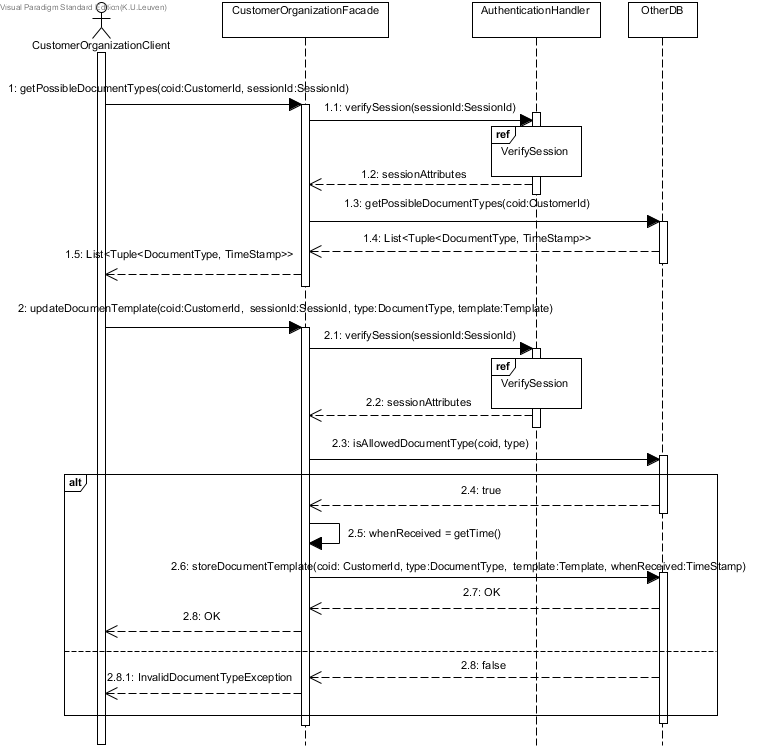
\includegraphics[width=\textwidth]{Seq_UC20UpdateDocumentTemplate.png}

    
    \caption{The system behavior for updating a document template.
        }\label{fig:seq_UC20UpdateDocumentTemplate}
\end{figure}

\subsection{Verifying a session}
Figure \ref{fig:seq_VerifySession} how it is verified whether a session is valid. The \texttt{AuthenticationHandler} uses the \texttt{SessionDB} to verify whether each incoming session identifier belongs to an existing session. If it belongs to an existing session, the corresponding session attributes are returned to the caller, otherwise an NoSuchSessionException is thrown.
\begin{figure}[!htp]
    \centering
    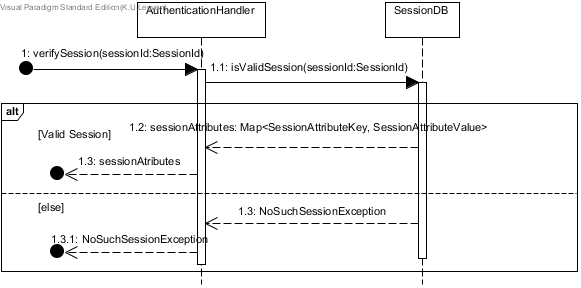
\includegraphics[width=\textwidth]{Seq_VerifySession.png}
    \caption{verifySession: sequence diagram depicting the verification whether a session is valid.
        }\label{fig:seq_VerifySession}
\end{figure}

\FloatBarrier

\subsection{Initiating document processing}
Figure \ref{fig:seq_UC3InitiateDocumentProcessing} shows how a customer organization initiates a batch of document processing jobs. Recurring and non-recurring batches are indicated using the \texttt{isRecurring} boolean value. If the batch is non-recurring, the customer organization can indicate another priority than the default priority of that customer organization if the batch should be handled with another priority than the default priority.  For recurring batches, it does not matter if a priority is given, as the default priority will be used. The customer organization also delivers the raw data as a \texttt{rawDataPackage}. After verification of the session identifier (figure \ref{fig:seq_VerifySession}), the \texttt{CustomerOrganizationFacade} generates a \texttt{TimeStamp} of the time when this method is called and forwards this together with all its arguments except for the \texttt{sessionid} to \texttt{RawDataHandler}, while also indicating if the batch is (non-)recurring.\\

Figure \ref{fig:seq_VerifyRawData} depicts the first part of the method call in the \texttt{RawDataHandler}, which will verify whether the raw data is valid. First, \texttt{RawDataHandler} checks whether the customer organization is allowed to generated the given document type. If it is allowed, the received raw data packet will be validated, e.g  there will be checked whether the content of the received Excel file can be read or whether a received XML file is correctly formatted. If it is not valid, an exception is thrown. Otherwise, depending on if the batch is  recurring, the \texttt{RawDataHandler} will query the SLA in the \texttt{OtherDB} to check if the number of raw data entries in the raw data package is allowed. If the number of entries exceeds this maximum, an exception is thrown. Next, each individual entry will be checked on validity, so the \texttt{RawdataHandler} knows which \texttt{RawData} entries are valid and which are not.\\

After verification, figure \ref{fig:seq_UC3InitiateDocumentProcessing} shows that the \texttt{RawDataHandler} will only use the given priority if the batch is non-recurring. Otherwise, it will use the default priority. The deadline of the document processing jobs is calculated and a \texttt{BatchMetaData} object is generated, bundling the information about the batch. The \texttt{RawDataHandler} will store the \texttt{RawData} entries and \texttt{BatchMetaData} in the \texttt{OtherDB}. It asks the \texttt{JobFacade} to create jobs for the valid raw data entries and to initiate document processing for those jobs. Finally, it will return the invalid raw data entries to the Customer Organization.\\

Figure \ref{fig:seq_CreateJobs} shows the \texttt{JobFacade} creating and storing jobs for the valid raw data entries, after which it inserts these jobs into the \texttt{Scheduler}.\\


\begin{figure}[!htp]
    \centering
    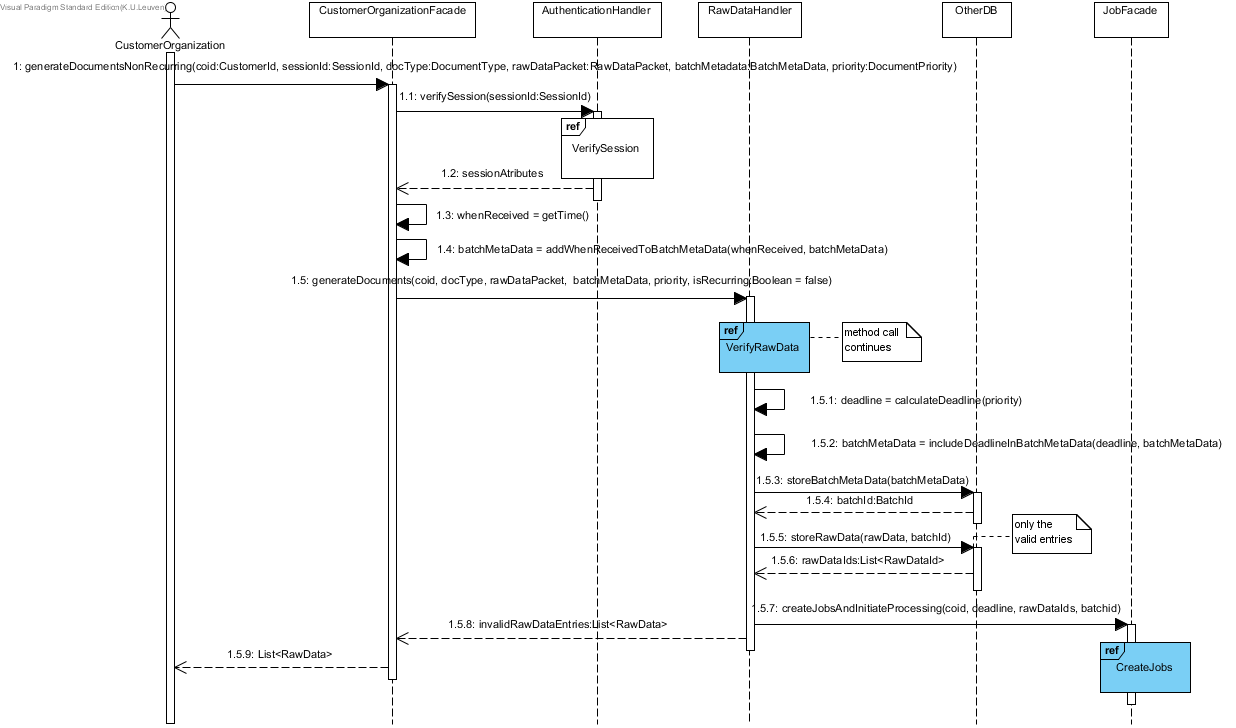
\includegraphics[width=0.8\textwidth]{Seq_UC3InitiateDocumentProcessing.png}
    \caption{VerifyRawData: verification whether the raw data is valid.
        }\label{fig:seq_UC3InitiateDocumentProcessing}
\end{figure}

\begin{figure}[!htp]
    \centering
    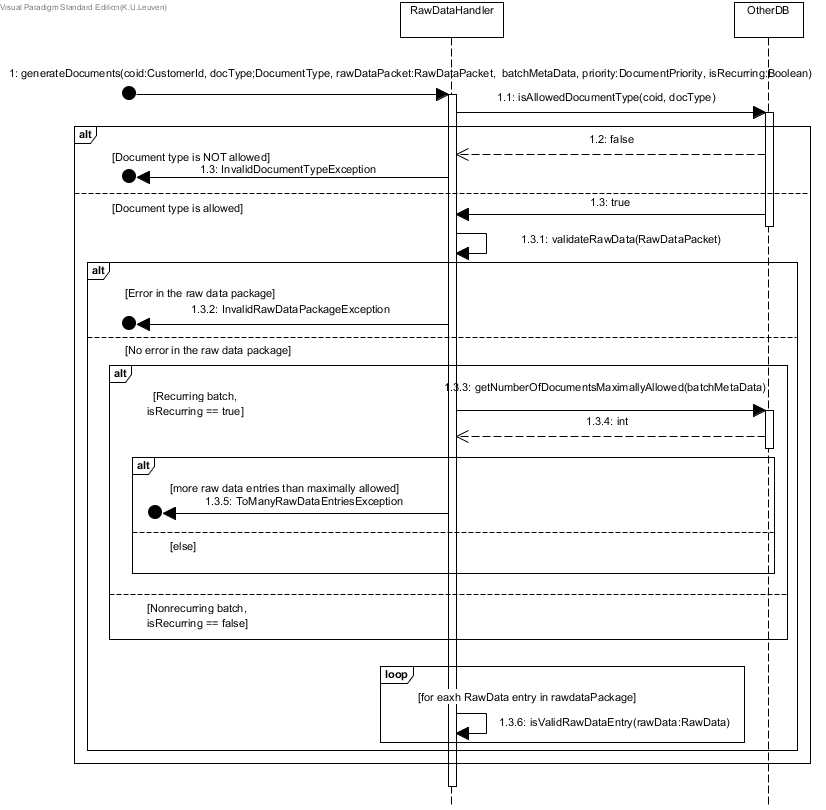
\includegraphics[width=\textwidth]{Seq_VerifyRawData.png}
    \caption{VerifyRawData: verification whether the raw data is valid.
        }\label{fig:seq_VerifyRawData}
\end{figure}

\begin{figure}[!htp]
    \centering
    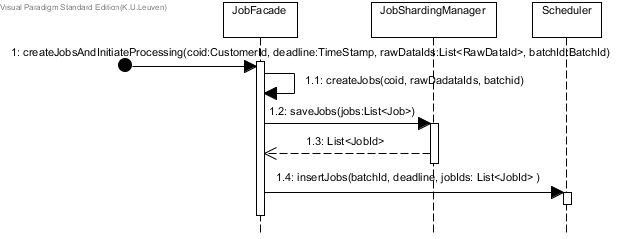
\includegraphics[width=\textwidth]{Seq_CreateJobs.png}
    \caption{CreateJobs: the \texttt{JobManager creates jobs and forwards them to be scheduled by the \texttt{Scheduler}}.
        }\label{fig:seq_CreateJobs}
\end{figure}

\subsection{Consult document in personal document store}
Shortly describe the scenario shown in this subsection.
Show the complete scenario using one or more sequence diagrams.

\begin{figure}[!htp]
    \centering
    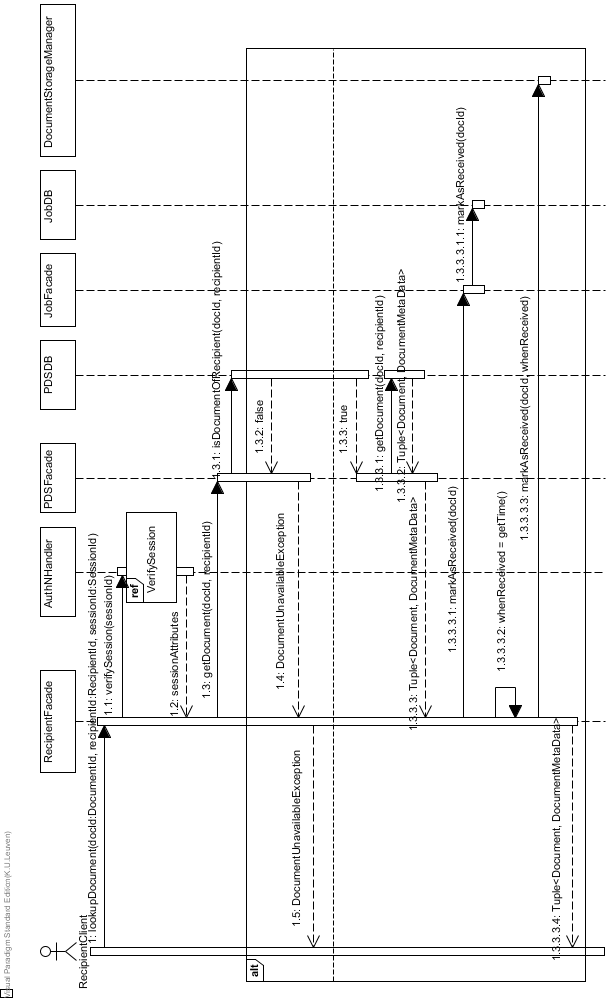
\includegraphics[width=0.8\textwidth]{Seq_UC14ConsultDocumentInPDS.png}
    \caption{A Registered Recipient consults a document in his or her personal document store.
        }\label{fig:seq_UC14ConsultdocumentInPDS}
\end{figure}

\FloatBarrier

\subsection{Delivering a document via the personal document store}
Shortly describe the scenario shown in this subsection.
Show the complete scenario using one or more sequence diagrams.

\begin{figure}[!htp]
    \centering
    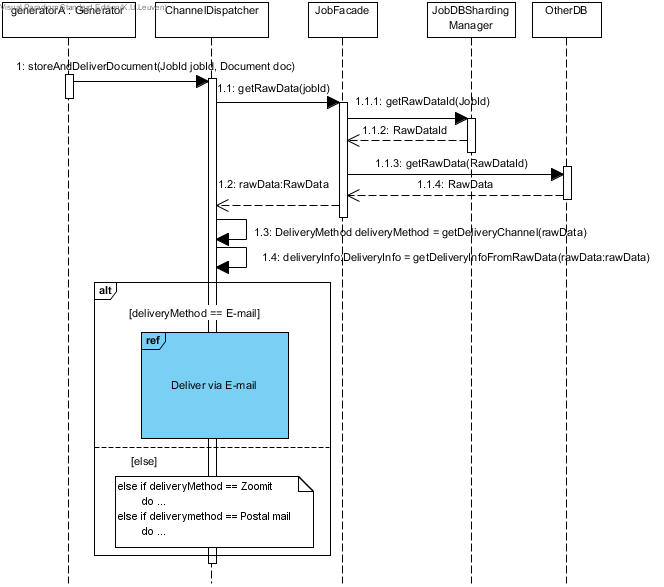
\includegraphics[width=\textwidth]{Seq_InitiateDocumentDelivery.png}
    \caption{The system behavior for the first scenario.
        }\label{fig:seq_InitiateDocumentdelivery}
\end{figure}

\begin{figure}[!htp]
    \centering
    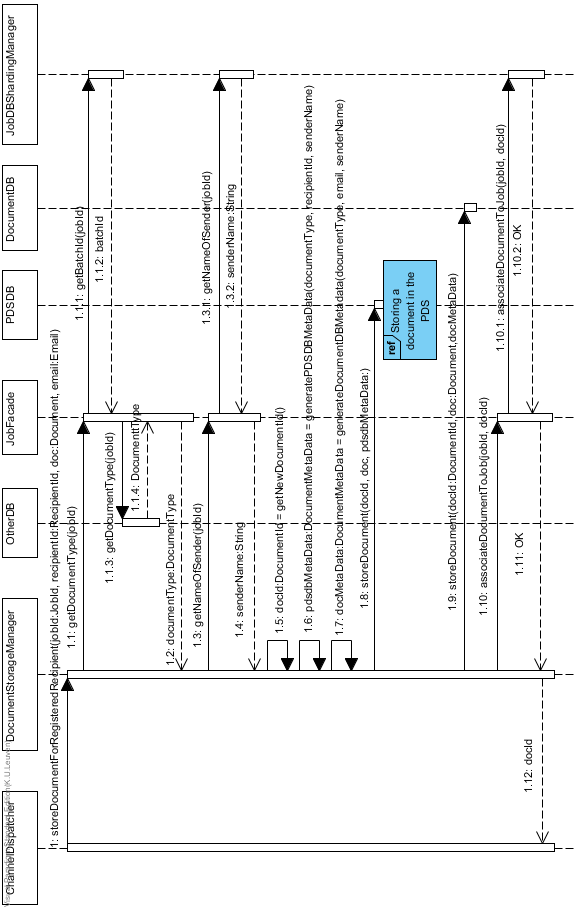
\includegraphics[width=0.8\textwidth]{Seq_StoreDocRegisteredRecipient.png}
    \caption{The system behavior for the first scenario.
        }\label{fig:seq_StoreDocRegisteredRecipient}
\end{figure}

\begin{figure}[!htp]
    \centering
    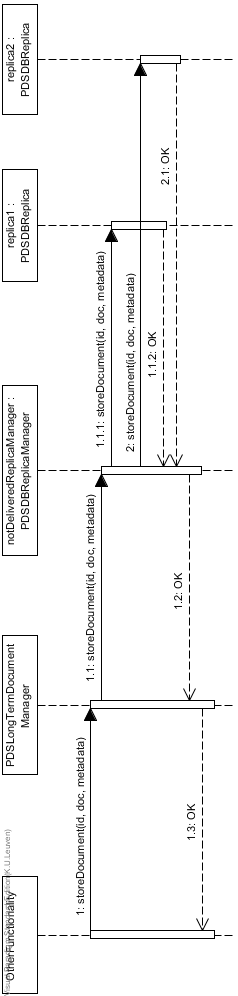
\includegraphics[width=0.3\textwidth]{Seq_StoreDocPDS.png}
    \caption{The system behavior for the first scenario.
        }\label{fig:seq_StoreDocPDS}
\end{figure}


\appendix
\section{Element catalog}\label{app:catalog}
In this section, we list all the components and the interfaces they provide. Per component, we describe its responsibilities, declare its super-component (if any) and list its sub-components (if any).



List all components and describe their responsibilities and provided
interfaces.
Per interface, list all methods using a Java-like syntax and describe their
effect and exceptions if any.
List all elements and interfaces alphabetically for ease of navigation.

\subsection{AuthenticationHandler}
\begin{itemize}
    \item \textbf{Description:} The \texttt{AuthenticationHandler} is responsible for authenticating Registered recipients and Customer organizations. The architecture does not specify the means of authentication (e.g. the type of credentials). The credentials are stored in the \texttt{UserDB}.
    \item \textbf{Super-component:} \texttt{UserFunctionality}
    \item \textbf{Sub-components:} None
\end{itemize}

\subsubsection*{Provided interfaces}
\begin{itemize}
    \item AuthN
    \begin{itemize}
        \item \texttt{RecipientId getRecipientId(SessionId sessionId) throws NoSuchSessionException}
        \begin{itemize}
            \item Effect: The \texttt{AuthenticationHandler} fetches and returns the Registered Recipient's identifier corresponding to the \texttt{sessionId} from the \texttt{SessionDB}.
            \item Exceptions:
            \begin{itemize}
                \item NoSuchSessionException: Thrown if no session exists with the given identifiers, or if the session belongs to a customer organization.
            \end{itemize}
		\end{itemize}
		
        \item \texttt{CustomerId getCustomerId(SessionId sessionId) throws NoSuchSessionException}
        \begin{itemize}
             \item Effect: The \texttt{AuthenticationHandler} fetches and returns the Customer Organization's identifier corresponding to the \texttt{sessionId} from the \texttt{SessionDB}.
             \item Exceptions:
             \begin{itemize}
                \item NoSuchSessionException: Thrown if no session exists with the given identifier, or if the session belongs to a registered recipient.
             \end{itemize}
        \end{itemize}
        
        \item \texttt{Boolean logout(SessionId sessionId)}
        \begin{itemize}
            \item Effect: The \texttt{AuthenticationHandler} will remove the session with the given id from the \texttt{SessionDB}. If no such session exists, nothing is changed and no exception is thrown.
            \item Exceptions: None
        \end{itemize}
        
        \item \texttt{SessionId login(Credentials credentials) throws InvalidCredentialsException}
        \begin{itemize}
            \item Effect: The \texttt{AuthenticationHandler} verifies the \texttt{credentials} using the \texttt{UserDB}. If they are correct, the \texttt{AuthenticationHandler} creates a new session using the \texttt{SessionDB}, stores the id of the user (i.e. the Registered Recipient id or Customer Organization id) as an attribute in this session and returns the id of the new session. The id of the user is present in the given credentials.
            \item Exceptions: 
            \begin{itemize}
                \item InvalidCredentialsException: Thrown if the given credentials are invalid.
             \end{itemize}
        \end{itemize}
    \end{itemize}
    
    
	\item CheckSession
    \begin{itemize}
        \item \texttt{Map<SessionAttributeKey, SessionAttributeValue> verifySession(SessionId sesionId) throws NoSuchsSessionException}
        \begin{itemize}
            \item Effect: The \texttt{AuthenticationHandler} verifies whether a session with the given id exists in the \texttt{SessionDB} and if so, returns all its associated attributes.
            \item Exceptions:
            \begin{itemize}
                \item NoSuchSessionException: Thrown if no session exists with the given identifiers.
             \end{itemize}
        \end{itemize}
    \end{itemize}	
\end{itemize}

\subsection{BillingManager}
\begin{itemize}
    \item \textbf{Description:} The \texttt{BillingManager} is responsible for all billing tasks. This includes billing the Customer Organization for the generation and delivery of non-recurring document processing jobs.
    \item \textbf{Super-component:} None
    \item \textbf{Sub-components:} None
\end{itemize}

\subsubsection*{Provided interfaces}
\begin{itemize}
    \item CostRegistrationMgmt
    \begin{itemize}
        \item \texttt{void addDocumentGenerationCost(CustomerId cuId, JobId jobId, DocumentPriority priority)}
        \begin{itemize}
            \item Effect: The \texttt{BillingManager} adds the cost for generation documents corresponding to the job identified by \texttt{jobId} to the bill of the customer organization identified by \texttt{cuId}. The document had a priority \texttt{priority}. This method is called by the \texttt{GenerationManager}.
            \item Exceptions: None
        \end{itemize}
        
		\item \texttt{void addDocumentDeliveryCostbyEmail(CustomerId cuId, JobId jobId)}       
        \begin{itemize}
            \item Effect: The \texttt{BillingManager} adds the cost for delivering the document by e-mail to the bill of the customer organization identified by \texttt{cuId}. The document corresponds to the job identified by \texttt{JobId}. This method is called by the \texttt{ChannelDispatcher}.
            \item Exceptions: None
        \end{itemize} 

		\item \texttt{void addDocumentDeliveryCostbyPrintAndPostalService(CustomerId cuId, JobId jobId)}       
        \begin{itemize}
            \item Effect: The \texttt{BillingManager} adds the cost for delivering the document by e-mail to the bill of the customer organization identified by \texttt{cuId}. The document corresponds to the job identified by \texttt{JobId}. This method is called by the \texttt{ChannelDispatcher}.
            \item Exceptions: None
        \end{itemize} 
        
		\item \texttt{void addDocumentDeliveryCostbyZoomit(CustomerId cuId, JobId jobId)}       
        \begin{itemize}
            \item Effect: The \texttt{BillingManager} adds the cost for delivering the document by Zoomit to the bill of the customer organization identified by \texttt{cuId}. The document corresponds to the job identified by \texttt{JobId}. This method is called by the \texttt{ChannelDispatcher}.
            \item Exceptions: None
        \end{itemize}                
    \end{itemize}
\end{itemize}

\subsection{ChannelDispatcher}
\begin{itemize}
    \item \textbf{Description:} The \texttt{ChannelDispatcher} is responsible for choosing the correct delivery channel for a generated document. It also forwards the document to the \texttt{DocumentStorageManager}, which will store the document.
    \item \textbf{Super-component:} \texttt{Deliveryfunctionality}
    \item \textbf{Sub-components:} None
\end{itemize}

\subsubsection*{Provided interfaces}
\begin{itemize}
    \item FinalizeDocument\\
    Note that the methods in this interface are made idempotent. The methods of this interface are called by \texttt{Generator} instances. 
    \begin{itemize}
        \item \texttt{void storeAndDeliverDocument(JobId jobid, Document doc)}
        \begin{itemize}
            \item Effect: The \texttt{ChannelDispatcher} will store the given document \texttt{document} and deliver it. This method is made idempotent. To filer duplicate method calls, it has the \texttt{JobId} of the document as an argument. This idempotence is to account for the case when case when a \texttt{Generator} fails after forwarding the document and before reporting completion to the \texttt{DocumentGenerationManager}. In this case, it can be that the \texttt{DocumentGenerationManager} restarts jobs for which a document has already been stored or delivered.
            \item Exceptions: None
		\end{itemize}
		
        \item \texttt{void generationError(JobId jobid, Error error)}
        \begin{itemize}
            \item Effect: Describe the effect of the operation
            \item Exceptions: None
        \end{itemize}
    \end{itemize}
\end{itemize}

\subsection{CustomerOrganizationClient}
\begin{itemize}
    \item \textbf{Description:} The \texttt{CustomerOrganizationClient} is external to the eDocs system and represents a client device of a Customer  Organization (i.e. Customer Administrator and Customer Information System) that communicates with the eDocs System.
    \item \textbf{Super-component:} None
    \item \textbf{Sub-components:} None
\end{itemize}

\subsubsection*{Provided interfaces}
\begin{itemize}
    \item InterfaceA
    \begin{itemize}
        \item \texttt{returntType1 operation1(ParamType param) throws SomeException}
        \begin{itemize}
            \item Effect: Describe the effect of the operation
            \item Exceptions:
            \begin{itemize}
                \item SomeException: Describe when the exception is thrown.
            \end{itemize}
		\end{itemize}
		
        \item \texttt{void operation2(ParamType2 param)}
        \begin{itemize}
            \item Effect: Describe the effect of the operation
            \item Exceptions: None
        \end{itemize}  
    \end{itemize}
\end{itemize}

\subsection{CustomerOrganizationFacade}
\begin{itemize}
    \item \textbf{Description:} The \texttt{CustomerOrganizationFacade} provides the main interface of the system to the Customer  Organization (i.e. Customer Administrator and Customer Information System).
    \item \textbf{Super-component:} \texttt{UserFunctionality}
    \item \textbf{Sub-components:} None
\end{itemize}

\subsubsection*{Provided interfaces}
\begin{itemize}
    \item AuthN
    \begin{itemize}
           \item \texttt{Boolean logout(SessionId sessionId)}
        \begin{itemize}
            \item Effect: The \texttt{AuthenticationHandler} will remove the session with the given id from the \texttt{SessionDB}. If no such session exists, nothing is changed and no exception is thrown.
            \item Exceptions: None
        \end{itemize}
        
        \item \texttt{SessionId login(Credentials credentials) throws InvalidCredentialsException}
        \begin{itemize}
            \item Effect: The \texttt{AuthenticationHandler} verifies the \texttt{credentials} using the \texttt{UserDB}. If they are correct, the \texttt{AuthenticationHandler} creates a new session using the \texttt{SessionDB}, stores the id of the user (i.e. the Registered Recipient id or Customer Organization id) as an attribute in this session and returns the id of the new session. The id of the user is present in the given credentials.
            \item Exceptions: 
            \begin{itemize}
                \item InvalidCredentialsException: Thrown if the given credentials are invalid.
             \end{itemize}
        \end{itemize}
     \end{itemize}  
      
    \item TemplateMgmt
    \begin{itemize}
    	\item \texttt{List<Tuple<DocumentType,TimeStamp>> getPossibleDocumentTypes(SessionId sessionId, CustomerId cuId) throws NotAuthenticatedException}
        \begin{itemize}
            \item Effect: The \texttt{CustomerOrganizationClient} will return a list of the document types that the customer organization is allowed to generate. It also indicates the current template for each document type by returning for each document type the time when the last template was uploaded.
            \item Exceptions:
            \begin{itemize}
            	\item NotAuthenticatedException: Thrown if the given session identifier is invalid.
            \end{itemize}
        \end{itemize}
        
   	\item \texttt{Boolean updateDocumentTemplate(SessionId sessionId, CustomerId cuId, DocumentType documentType, Template template) throws NotAuthenticatedException, InvalidDocumentTypeException}
        \begin{itemize}
            \item Effect: The \texttt{CustomerOrganizationClient} will update the current template for the given \texttt{documentType} to the given \texttt{template} for the customer organization identified by \texttt{cuId}. Returns true when it succeeds.
            \item Exceptions:
            \begin{itemize}
            	\item NotAuthenticatedException: Thrown if the given session identifier is invalid.
            	\item InvalidDocumentTypeException: Thrown if the given document type is invalid or not allowed for the given customer organization.
            \end{itemize}
        \end{itemize}        
    \end{itemize}
    
    \item InitiateDocumentProcessing
    \begin{itemize}
    	\item \texttt{List<RawData> initiateDocumentProcessing(CustomerId cuid, SessionId sessionId, \\DocumentType docType, RawDataPacket rawDataPacket, \\ DocumentPriority priority, Boolean isRecurring) throws NotAuthenticatedException,\\ InvalidDocumentTypeException, InvalidRawDataPackageException, ToManyRawDataEntriesException }
    	 \begin{itemize}
            \item Effect: The \texttt{CustomerOrganizationFacade} gets an indication from a customer organization with customer identifier \texttt{cuid} to start a batch of document processing jobs. The documents to be generated should be of document type \texttt{docType}. The boolean \texttt{isRecurring} indicates whether the batch is recurring or non-recurring. The information necessary to generate the documents is given in  a \texttt{RawDataPacket} containing all the info about the raw data entries of the batch. After verification of the session identifier, the \texttt{CustomerOrganizationFacade} generates a \texttt{TimeStamp} of the time when this method is called and forwards it together with most of its arguments to the \texttt{RawDataHandler}.
            \item Exceptions:
            \begin{itemize}
            	\item NotAuthenticatedException: Thrown if the given session identifier is invalid.
            	\item InvalidDocumentTypeException: Thrown if the given document type is invalid or not allowed for the given customer organization.
            	\item InvalidRawDataPackageException: Thrown if the raw data package contains an error (e.g. an invalid Excel file or incorrectly formatted XML).
            	\item ToManyRawDataEntriesException: Thrown if the batch is a recurring batch and contains more raw data entries than maximally allowed for this batch.
            \end{itemize}
        \end{itemize}  	
    \end{itemize}
\end{itemize}

\subsection{Completer}
\begin{itemize}
    \item \textbf{Description:} The \texttt{Completer} is responsible for fetching the raw data an applicable meta-data for a group of \texttt{JobIds} when a \texttt{Generator} instance requires a new group of jobs.
    \item \textbf{Super-component:} \texttt{DocumentGenerationManager}
    \item \textbf{Sub-components:} None
\end{itemize}

\subsubsection*{Provided interfaces}
\begin{itemize}
    \item Complete
    \begin{itemize}
        \item \texttt{CompletePartialBatchData getComplete(BatchId batchId, List<JobId> jobIds )}
        \begin{itemize}
            \item Effect: The \texttt{Completer} fetches data needed by a \texttt{Generator} for generation of the documents corrseponding to the\texttt{JobIds} belonging to the same batch, which is identified by \texttt{BatchId}.
            \item Exceptions: None
        \end{itemize}
    \end{itemize}
\end{itemize}

\subsection{DocumentDB}
\begin{itemize}
    \item \textbf{Description:} The \texttt{DocumentDB} is responsible  for actually storing all the documents. It stores documents regardless of the fact of a document is also stored in the \texttt{PDSDB} It receives read and write requests from the \texttt{DocumentStoragManager}.
    \item \textbf{Super-component:} None
    \item \textbf{Sub-components:} \texttt{DocumentDBShardingManager} and \texttt{DocumentDBShard}
\end{itemize}

\subsubsection*{Provided interfaces}
\begin{itemize}
    \item InterfaceA
    \begin{itemize}
        \item \texttt{returntType1 operation1(ParamType param) throws SomeException}
        \begin{itemize}
            \item Effect: Describe the effect of the operation
            \item Exceptions:
            \begin{itemize}
                \item SomeException: Describe when the exception is thrown.
            \end{itemize}
		\end{itemize}
        \item \texttt{void operation2(ParamType2 param)}
        \begin{itemize}
             \item Effect: Describe the effect of the operation
             \item Exceptions: None
        \end{itemize} 
    \end{itemize}

    \item InterfaceB
    \begin{itemize}
        \item \texttt{returntType2 operation3()}
        \begin{itemize}
            \item Effect: Describe the effect of the operation
            \item Exceptions: None
        \end{itemize}
    \end{itemize}
\end{itemize}

\subsection{DocumentDBShard}
\begin{itemize}
    \item \textbf{Description:} A \texttt{DocumentDBShard} is responsible for storing a partition of all the documents.
    \item \textbf{Super-component:} \texttt{DocumentDB}
    \item \textbf{Sub-components:} None
\end{itemize}

\subsubsection*{Provided interfaces}
\begin{itemize}
    \item InterfaceA
    \begin{itemize}
        \item \texttt{returntType1 operation1(ParamType param) throws SomeException}
        \begin{itemize}
            \item Effect: Describe the effect of the operation
            \item Exceptions:
            \begin{itemize}
                \item SomeException: Describe when the exception is thrown.
            \end{itemize}
		\end{itemize}
        \item \texttt{void operation2(ParamType2 param)}
        \begin{itemize}
            \item Effect: Describe the effect of the operation
            \item Exceptions: None
        \end{itemize}
    \end{itemize}

    \item InterfaceB
    \begin{itemize}
        \item \texttt{returntType2 operation3()}
        \begin{itemize}
            \item Effect: Describe the effect of the operation
            \item Exceptions: None
        \end{itemize}
    \end{itemize}
\end{itemize}

\subsection{DocumentDBShardingManager}
\begin{itemize}
    \item \textbf{Description:} The \texttt{DocumentDBShardingManager} manages the storage of the documents over multiple \texttt{DocumentDBShards}.
    \item \textbf{Super-component:} The \texttt{DocumentDB}
    \item \textbf{Sub-components:} None
\end{itemize}

\subsubsection*{Provided interfaces}
\begin{itemize}
    \item InterfaceA
    \begin{itemize}
        \item \texttt{returntType1 operation1(ParamType param) throws SomeException}
        \begin{itemize}
            \item Effect: Describe the effect of the operation
            \item Exceptions:
            \begin{itemize}
                \item SomeException: Describe when the exception is thrown.
            \end{itemize}
		\end{itemize}
        \item \texttt{void operation2(ParamType2 param)}
        \begin{itemize}
            \item Effect: Describe the effect of the operation
            \item Exceptions: None
        \end{itemize}
    \end{itemize}

    \item InterfaceB
    \begin{itemize}
        \item \texttt{returntType2 operation3()}
        \begin{itemize}
            \item Effect: Describe the effect of the operation
            \item Exceptions: None
        \end{itemize}
    \end{itemize}
\end{itemize}

\subsection{DocumentGenerationManager}
\begin{itemize}
    \item \textbf{Description:} The \texttt{DocumentGenerationManager} monitors the availability of the \texttt{Generator} components using the Ping interface. The \texttt{DocumentGenerationManager} keeps track of the jobs assigned to and being processed by the \texttt{Generators}. To minimize the overhead of the job coordination, the \texttt{DocumentGenerationManager} assigns jobs to the \texttt{Generators} in groups of more than one job that are part of the same batch. If a \texttt{Generator} fails to complete its jobs, the \texttt{DocumentGenerationManager} can restart these failed jobs. \\ It prioritizes jobs based on thei deadlines ansd schedules them according to \emph{P1}.
    \item \textbf{Super-component:} None
    \item \textbf{Sub-components:} \texttt{Completer}, \texttt{GenerationManager}, \texttt{KeyCache}, \texttt{Scheduler}, \texttt{TemplateCache}
\end{itemize}

\subsubsection*{Provided interfaces}
\begin{itemize}
    \item InsertJobs
    \begin{itemize}
        \item \texttt{returntType1 operation1(ParamType param) throws SomeException}
        \begin{itemize}
            \item Effect: Describe the effect of the operation
            \item Exceptions:
            \begin{itemize}
                \item SomeException: Describe when the exception is thrown.
            \end{itemize}
        \end{itemize}
    \end{itemize}

    \item NotifyCompleted
    \begin{itemize}
        \item \texttt{void notifyCompletedAndGiveMeMore(GeneratorId id)}
        \begin{itemize}
            \item Effect: The \texttt{DocumentGenerationManager} gets notified that the document processing jobs assigned to the \texttt{Generator} identified by an \texttt{id} are completed. 
            %It looks up the \texttt{JobIds} of the jobs assigned to the \texttt{Generator}. It notifies the \texttt{Scheduler} that the job
            \item Exceptions: None
        \end{itemize}
        
        \item \texttt{void notifyCompletedAndIAmShuttingDown(GeneratorId id)}
        \begin{itemize}
            \item Effect: The \texttt{DocumentGenerationManager} gets notified that the document processing jobs assigned to the \texttt{Generator} identified by an \texttt{id} are completed. 
            \item Exceptions: None
        \end{itemize}
    \end{itemize}
\end{itemize}

\subsection{DocumentStorageCache}
\begin{itemize}
    \item \textbf{Description:} The \texttt{DocumentStorageCache} is responsible for storing the \texttt{DocumentIds} and \texttt{RecipientIds} when the \texttt{PDSDB} fails. According to Av2, the system should temporarily store at least 3 hours of documents to be delivered via the personal document store. When the \texttt{PDSDB} fails, the documents that are supposed to also be saved in the \texttt{PDSDB} are saved in the \texttt{DocumentDB}, just as usual. But in this case the \texttt{DocumentStorageManager} also stores the \texttt{DocumentIds} and \texttt{RecipientIds} of those documents in the \texttt{DocumentStorageCache} for at least 3 hours. This way, the \texttt{DocumentStorageManager} can transfer these documents from the \texttt{DocumentDB} to the \texttt{PDSDB} using this information if the \texttt{PDSDB} comes back online within 3 hours. The requirements do not specify what happens after 3 hours, so in this architecture, the behaviour after those 3 hours is undefined.
    \item \textbf{Super-component:} \texttt{DocumentStorageFunctionality}
    \item \textbf{Sub-components:} None
\end{itemize}

\subsubsection*{Provided interfaces}
\begin{itemize}
    \item InterfaceA
    \begin{itemize}
        \item \texttt{returntType1 operation1(ParamType param) throws SomeException}
        \begin{itemize}
            \item Effect: Describe the effect of the operation
            \item Exceptions:
            \begin{itemize}
                \item SomeException: Describe when the exception is thrown.
            \end{itemize}
		\end{itemize}
        \item \texttt{void operation2(ParamType2 param)}
        \begin{itemize}
            \item Effect: Describe the effect of the operation
            \item Exceptions: None
        \end{itemize}
    \end{itemize}

    \item InterfaceB
    \begin{itemize}
        \item \texttt{returntType2 operation3()}
        \begin{itemize}
            \item Effect: Describe the effect of the operation
            \item Exceptions: None
        \end{itemize}
    \end{itemize}
\end{itemize}


\subsection{DocumentStorageFunctionality}
\begin{itemize}
    \item \textbf{Description:} The \texttt{DocumentStorageManager} is responsible for storing the generated documents in the correct database. If the document belongs to a registered recipient, it sends a write request to both the \texttt{DocumentDB} and the \texttt{PDSDB}. Otherwise, it only sends a write request to the \texttt{DocumentDB}, which stores all the documents.\\
    It is also responsible for copying documents from the \texttt{DocumentDB} to the \texttt{PDSDB} when an Unregistered Recipient registers to the eDocs system.\\ Another responsibility of the \texttt{DeliveryFunctionality} is storing at least 3 hours of documents when the \texttt{PDSDB} fails.
    \item \textbf{Super-component:} None
    \item \textbf{Sub-components:} \texttt{DocumentStorageCache} and \texttt{DocumentStorageManager}
\end{itemize}

\subsubsection*{Provided interfaces}
\begin{itemize}
    \item InterfaceA
    \begin{itemize}
        \item \texttt{returntType1 operation1(ParamType param) throws SomeException}
        \begin{itemize}
            \item Effect: Describe the effect of the operation
            \item Exceptions:
            \begin{itemize}
                \item SomeException: Describe when the exception is thrown.
            \end{itemize}
		\end{itemize}
        \item \texttt{void operation2(ParamType2 param)}
        \begin{itemize}
            \item Effect: Describe the effect of the operation
            \item Exceptions: None
        \end{itemize}
    \end{itemize}

    \item InterfaceB
    \begin{itemize}
        \item \texttt{returntType2 operation3()}
        \begin{itemize}
            \item Effect: Describe the effect of the operation
            \item Exceptions: None
        \end{itemize}
    \end{itemize}
\end{itemize}


\subsection{DocumentStorageManager}
\begin{itemize}
    \item \textbf{Description:} The \texttt{DocumentStorageManager} is responsible for storing the generated documents in the correct database. If the document belongs to a registered recipient, it sends a write request to both the \texttt{DocumentDB} and the \texttt{PDSDB}. Otherwise, it only sends a write request to the \texttt{DocumentDB}, which stores all the documents.\\
    It is also responsible for copying documents from the \texttt{DocumentDB} to the \texttt{PDSDB} when an Unregistered Recipient registers to the eDocs system.\\ Another responsibility of the \texttt{DocumentStorageManager} is storing at least 3 hours of documents when the \texttt{PDSDB} fails.
    \item \textbf{Super-component:} \texttt{DocumentStoragefunctionlity}
    \item \textbf{Sub-components:} None
\end{itemize}

\subsubsection*{Provided interfaces}
\begin{itemize}
    \item DocumentStorageMgmt
    \begin{itemize}
        \item \texttt{void markAsReceived(DocumentId documentId, TimeStamp whenReceived)}
        \begin{itemize}
            \item Effect: The \texttt{DocumentStorageManager} marks the document identified by the given document identifier as received, by storing the given time in the document meta-data of the document. The given time is the time when the recipient should have received the document. Note that this method only has effect the first time it is called for a valid document identifier and time stamp.
            \item Exceptions: None
        \end{itemize}
    \end{itemize}
\end{itemize}

\subsection{DeliveryFunctionality}
\begin{itemize}
    \item \textbf{Description:} The \texttt{DeliveryFunctionality} is responsible  for delivering the documents generated by eDocs to the recipients. 
    \item \textbf{Super-component:} \texttt{ChannelDispatcher}, \texttt{EmailFacade}, \texttt{Print\&PostalServiceFacade}, \texttt{ZoomitFacade} and \texttt{ZoomitDeliveryCache}
    \item \textbf{Sub-components:} the direct sub-components, if any.
\end{itemize}

\subsubsection*{Provided interfaces}
\begin{itemize}
    \item InterfaceA
    \begin{itemize}
        \item \texttt{returntType1 operation1(ParamType param) throws SomeException}
        \begin{itemize}
            \item Effect: Describe the effect of the operation
            \item Exceptions:
            \begin{itemize}
                \item SomeException: Describe when the exception is thrown.
            \end{itemize}
        \end{itemize}
    \end{itemize}

    \item InterfaceB
    \begin{itemize}
        \item \texttt{returntType2 operation3()}
        \begin{itemize}
            \item Effect: Describe the effect of the operation
            \item Exceptions: None
        \end{itemize}
    \end{itemize}
\end{itemize}

\subsection{EDocsAdminClient}
\begin{itemize}
    \item \textbf{Description:} The \texttt{EDocsAdminClient} is external to the eDocs system and represents a client device of an administrator of eDocs that communicates with the eDocs System.
    \item \textbf{Super-component:} None
    \item \textbf{Sub-components:} None
\end{itemize}

\subsubsection*{Provided interfaces}
\begin{itemize}
    \item InterfaceA
    \begin{itemize}
        \item \texttt{returntType1 operation1(ParamType param) throws SomeException}
        \begin{itemize}
            \item Effect: Describe the effect of the operation
            \item Exceptions:
            \begin{itemize}
                \item SomeException: Describe when the exception is thrown.
            \end{itemize}
		\end{itemize}
        \item \texttt{void operation2(ParamType2 param)}
        \begin{itemize}
            \item Effect: Describe the effect of the operation
            \item Exceptions: None
        \end{itemize}
    \end{itemize}

    \item InterfaceB
    \begin{itemize}
        \item \texttt{returntType2 operation3()}
        \begin{itemize}
            \item Effect: Describe the effect of the operation
            \item Exceptions: None
        \end{itemize}
    \end{itemize}
\end{itemize}

\subsection{EmailChannel}
\begin{itemize}
    \item \textbf{Description:} The \texttt{EmailChannel} is responsible for the delivery emails.
It is external to the eDocs system and represents a mail server of an e-mail provider.
    \item \textbf{Super-component:} None
    \item \textbf{Sub-components:} None.
\end{itemize}

\subsubsection*{Provided interfaces}
\begin{itemize}
    \item InterfaceA
    \begin{itemize}
        \item \texttt{returntType1 operation1(ParamType param) throws SomeException}
        \begin{itemize}
            \item Effect: Describe the effect of the operation
            \item Exceptions:
            \begin{itemize}
                \item SomeException: Describe when the exception is thrown.
            \end{itemize}
		\end{itemize}
        \item \texttt{void operation2(ParamType2 param)}
        \begin{itemize}
            \item Effect: Describe the effect of the operation
            \item Exceptions: None
        \end{itemize}
    \end{itemize}

    \item InterfaceB
    \begin{itemize}
        \item \texttt{returntType2 operation3()}
        \begin{itemize}
            \item Effect: Describe the effect of the operation
            \item Exceptions: None
        \end{itemize}
    \end{itemize}
\end{itemize}

\subsection{EmailFacade}
\begin{itemize}
    \item \textbf{Description:} The \texttt{EmailFacade} is responsible for creating and sending emails used in the delivery of documents. It will send documents to  Unregistered recipients by e-mail when receipt tracking is turned off. When receipt tracking is turned on for an Unregistered Recipient, it will send an e-mail containing a short description of the received document and a unique link, which can be followed to get document. For Registered Recipients, it will send an e-mail containing a short description of the document and a link to the document. It also marks jobs as sent using the \texttt{JobManager}.
    \item \textbf{Super-component:} \texttt{DeliveryFunctionality}
    \item \textbf{Sub-components:} None
\end{itemize}

\subsubsection*{Provided interfaces}
\begin{itemize}
    \item InterfaceA
    \begin{itemize}
        \item \texttt{returntType1 operation1(ParamType param) throws SomeException}
        \begin{itemize}
            \item Effect: Describe the effect of the operation
            \item Exceptions:
            \begin{itemize}
                \item SomeException: Describe when the exception is thrown.
            \end{itemize}
        \end{itemize}
    \end{itemize}

    \item InterfaceB
    \begin{itemize}
        \item \texttt{returntType2 operation3()}
        \begin{itemize}
            \item Effect: Describe the effect of the operation
            \item Exceptions: None
        \end{itemize}
    \end{itemize}
\end{itemize}

\subsection{Generator}
\begin{itemize}
    \item \textbf{Description:} A \texttt{Generator} generates the documents and forwards them to \texttt{DeliveryFunctionality} to store and deliver them. Its availability is monitored by the \texttt{DocumenGenerationManager} with the Ping interface. A \texttt{Generator} is also responsible of notifying the \texttt{NotificationHandler} that it does not have all of the data required to fill in the template.
    \item \textbf{Super-component:} None
    \item \textbf{Sub-components:} None
\end{itemize}

\subsubsection*{Provided interfaces}
\begin{itemize}
    \item AssignJobs
    \begin{itemize}
        \item \texttt{void assignJobs(CompletePartialBatchData batchData)}
        \begin{itemize}
            \item Effect: Describe the effect of the operation
            \item Exceptions:
            \begin{itemize}
                \item SomeException: Describe when the exception is thrown.
            \end{itemize}
        \end{itemize}
    \end{itemize}

    \item Startup/ShutDown
    \begin{itemize}
        \item \texttt{void startUp(GeneratorId generatorId)}
        \begin{itemize}
            \item Effect: Starts up the \texttt{Generator} instance an gives it the given \texttt{GeneratorId}. 
            \item Exceptions: None
        \end{itemize}
        
          \item \texttt{void shutDown()}
        \begin{itemize}
            \item Effect: The \texttt{Generator} completes its assigned group of document generation jobs and report back completion to the \texttt{DocumentGenerationManager}, after which is shuts down.
            \item Exceptions: None
        \end{itemize}
    \end{itemize}
    
    \item Ping
    \begin{itemize}
        \item \texttt{Echo ping()}
        \begin{itemize}
            \item Effect: The \texttt{Generator} will respond to the ping request by sending an echo response. This is used by the \texttt{GeneratorManager} to check whether the \texttt{Generator} is available.
            \item Exceptions: None
        \end{itemize}
    \end{itemize}
\end{itemize}
\subsection{GeneratorManager}
\begin{itemize}
    \item \textbf{Description:} The \texttt{GenerationManager} is responsible for monitoring the \texttt{Generator} instances. It starts up or shuts down these instances based on the number of required instances indicated by the \texttt{Scheduler}.
    \item \textbf{Super-component:}  \texttt{DocumentGenerationManager}
    \item \textbf{Sub-components:} None
\end{itemize}

\subsubsection*{Provided interfaces}
\begin{itemize}
    \item NotifyCompleted
    \begin{itemize}
        \item \texttt{void notifyCompletedAndGiveMeMore(GeneratorId id)}
        \begin{itemize}
            \item Effect: The \texttt{DocumentGenerationManager} gets notified that the document processing jobs assigned to the \texttt{Generator} identified by an \texttt{id} are completed. 
            %It looks up the \texttt{JobIds} of the jobs assigned to the \texttt{Generator}. It notifies the \texttt{Scheduler} that the job
            \item Exceptions: None
        \end{itemize}
    \end{itemize}
\end{itemize}

\subsection{JobDBShard}
\begin{itemize}
    \item \textbf{Description:} The \texttt{JobDBShard} is responsible for storing partition of all the jobs.
    \item \textbf{Super-component:} \texttt{JobManager}
    \item \textbf{Sub-components:} None
\end{itemize}

\subsubsection*{Provided interfaces}
\begin{itemize}
    \item InterfaceA
    \begin{itemize}
        \item \texttt{returntType1 operation1(ParamType param) throws SomeException}
        \begin{itemize}
            \item Effect: Describe the effect of the operation
            \item Exceptions:
            \begin{itemize}
                \item SomeException: Describe when the exception is thrown.
            \end{itemize}
		\end{itemize}
        \item \texttt{void operation2(ParamType2 param)}
        \begin{itemize}
            \item Effect: Describe the effect of the operation
            \item Exceptions: None
        \end{itemize}
    \end{itemize}

    \item InterfaceB
    \begin{itemize}
        \item \texttt{returntType2 operation3()}
        \begin{itemize}
            \item Effect: Describe the effect of the operation
            \item Exceptions: None
        \end{itemize}
    \end{itemize}
\end{itemize}

\subsection{JobDBShardingManager}
\begin{itemize}
    \item \textbf{Description:} The \texttt{JobDBShardingManager} manages the storage of the documents over multiple \texttt{JobDBShards}.
    \item \textbf{Super-component:} \texttt{JobManager}
    \item \textbf{Sub-components:} None
\end{itemize}

\subsubsection*{Provided interfaces}
\begin{itemize}
    \item JobDBMgmt
    \begin{itemize}
	    \item \texttt{RawData getRawData(JobId jobId)}
        \begin{itemize}
            \item Effect: The \texttt{JobDBShardingManager} returns the raw data entry corresponding to the job identified by the given job identifier.
            \item Exceptions: None
        \end{itemize}    
    
     	\item \texttt{void markAsReceived(DocumentId documentId) throws NoSuchJobExceptionException}
    	\begin{itemize}
    		\item Effect: The \texttt{JobFacade} marks the job corresponding to the document identified by the given document identifier as received by the recipient.
    		\item Exceptions:
    		\begin{itemize}
    			\item NoSuchJobException: Thrown if the \texttt{JobFacade} cannot find a job associated to a document identified by the given document identifier.
    		\end{itemize}
    	\end{itemize}
    \end{itemize}
\end{itemize}


\subsection{JobFacade}
\begin{itemize}
    \item \textbf{Description:} The \texttt{JobFacade} is responsible creating jobs and storing them using the \texttt{JobDBShadingManager} over different \texttt{JobDBShards}. It is responsible for retrieving data connected to a specific job. It can retrieve the raw data or customer organization info for specific jobs. The \texttt{JobFacade} is also used for marking jobs as sent and received.
    \item \textbf{Super-component:} \texttt{JobManager}
    \item \textbf{Sub-components:} None
\end{itemize}

\subsubsection*{Provided interfaces}
\begin{itemize}
    \item SetStatus
    \begin{itemize}
        \item \texttt{void setJobStatusAsTemporarilyFailed(List<JobId> statusesOfJobs)}
        \begin{itemize}
            \item Effect: The \texttt{JobManager} marks the job as ``temporarily failed'' for each of the jobs identified by the given \texttt{JobIds}. Used by the \texttt{DocumentGenerationManager} for jobs that where assigned to a failed \texttt{Generator} instance.
            \item Exceptions: None
        \end{itemize}
    \end{itemize}
    
	\item GetBatchData
    \begin{itemize}
        \item \texttt{RawData getRawData(JobId jobId)}
        \begin{itemize}
            \item Effect: The \texttt{JobFacade} returns the raw data entry corresponding to the job identified by the given job identifier.
            \item Exceptions: None
        \end{itemize}
        
        
        
        \item \texttt{Tuple<JobId, RawData> getRawData(List<JobId> jobIds)}
        \begin{itemize}
            \item Effect: Describe the effect of the operation
            \item Exceptions: None
        \end{itemize}
        \item \texttt{BatchMetaData getMetaData(BatchId batchId)}
        \begin{itemize}
            \item Effect: Describe the effect of the operation
            \item Exceptions: None
        \end{itemize}
    \end{itemize}  
    
    \item JobMgmt
    \begin{itemize}
    	\item \texttt{void createJobsAndInitiateProcessing(Customerid cuid, TimeStamp deadline, List<rawdataId> rawDataIds, batchId batchId)}
    	\begin{itemize}
            \item Effect: The \texttt{JobFacade} creates a job for each of the raw data identifiers it gets as an argument. The job contains the time of deadline for the document processing job and the batch identifier. It stores the jobs and inserts the jobs in the \texttt{Scheduler}, together with their deadline and batch identifier.
            \item Exceptions: None
        \end{itemize}
    	
    	\item \texttt{void markAsReceived(DocumentId documentId) throws NoSuchJobExceptionException}
    	\begin{itemize}
    		\item Effect: The \texttt{JobFacade} marks the job corresponding to the document identified by the given document identifier as received by the recipient.
    		\item Exceptions:
    		\begin{itemize}
    			\item NoSuchJobException: Thrown if the \texttt{JobFacade} cannot find a job associated to a document identified by the given document identifier.
    		\end{itemize}
    	\end{itemize}
    \end{itemize}
\end{itemize}

\subsection{JobManager}
\begin{itemize}
    \item \textbf{Description:} The \texttt{JobManager} is responsible creating jobs and storing them. It is responsible for retrieving data connected to a specific job. It can retrieve the raw data or customer organization info for specific jobs. The \texttt{JobFacade} is also used for marking jobs as sent and received.
    \item \textbf{Super-component:} None
    \item \textbf{Sub-components:} \texttt{JobFacade}, \texttt{JobDBShardingManager} and \texttt{JobDBShard}
\end{itemize}

\subsubsection*{Provided interfaces}
\begin{itemize}
    \item SetStatus
    \begin{itemize}
        \item \texttt{void setJobStatusAsTemporarilyFailed(List<JobId> statusesOfJobs)}
        \begin{itemize}
            \item Effect: The \texttt{JobManager} marks the job as ``temporarily failed'' for each of the jobs identified by the given \texttt{JobIds}. Used by the \texttt{DocumentGenerationManager} for jobs that where assigned to a failed \texttt{Generator} instance.
            \item Exceptions: None
        \end{itemize}
    \end{itemize}
    
	\item GetBatchData
    \begin{itemize}
        \item \texttt{RawData getRawData(JobId jobId)}
        \begin{itemize}
            \item Effect: The \texttt{JobManager} returns the raw data entry corresponding to the job identified by the given job identifier.
            \item Exceptions: None
        \end{itemize}    
    
        \item \texttt{Tuple<JobId, RawData> getRawData(List<JobId> jobIds)}
        \begin{itemize}
            \item Effect: Describe the effect of the operation
            \item Exceptions: None
        \end{itemize}
        \item \texttt{BatchMetaData getMetaData(BatchId batchId)}
        \begin{itemize}
            \item Effect: Describe the effect of the operation
            \item Exceptions: None
        \end{itemize}
    \end{itemize}    

    \item JobMgmt
    \begin{itemize}
    	\item \texttt{void createJobsAndInitiateProcessing(Customerid cuid, TimeStamp deadline, List<rawdataId> rawDataIds, batchId batchId)}
    	\begin{itemize}
            \item Effect: The \texttt{JobManager} creates a job for each of the raw data identifiers it gets as an argument. The job contains the time of deadline for the document processing job and the batch identifier. It stores the jobs and inserts the jobs in the \texttt{Scheduler}, together with their deadline and batch identifier.
            \item Exceptions: None
        \end{itemize}
    	
    	\item \texttt{void markAsReceived(DocumentId documentId) throws NoSuchJobExceptionException}
    	\begin{itemize}
    		\item Effect: The \texttt{JobManager} marks the job corresponding to the document identified by the given document identifier as received by the recipient.
    		\item Exceptions:
    		\begin{itemize}
    			\item NoSuchJobException: Thrown if the \texttt{JobManager} cannot find a job associated to a document identified by the given document identifier.
    		\end{itemize}
    	\end{itemize}
    \end{itemize}     
\end{itemize}

\subsection{KeyCache}
\begin{itemize}
    \item \textbf{Description:} The \texttt{KeyCache} caches the keys which are most recently used for document generation. The \texttt{Completer} has to fetch a key every time a \texttt{Generator} instance requests new jobs, while the key will be the same for all jobs belonging to the same batch. The \texttt{KeyCache} avoids that the key storage system becomes a bottleneck for document generations. The keys are cached based on the \texttt{CustomerId} of a Customer Organization.
    \item \textbf{Super-component:}  \texttt{DocumentGenerationManager}.
    \item \textbf{Sub-components:} None
\end{itemize}

\subsubsection*{Provided interfaces}
\begin{itemize}
    \item GetKey
    \begin{itemize}
        \item \texttt{Key getKey(CustomerId customerId) throws NoSuchKeyException}
        \begin{itemize}
            \item Effect: The \texttt{KeyCache} looks into its cache for the \texttt{Key} belonging to the customer organisation with id \texttt{customerId}. If the \texttt{Key} is in its cache, it returns it. If the \texttt{Key} is not in its cache, it asks \texttt{OtherDB} for the \texttt{Key} and stores it in its cache, after which it returns that \texttt{Key}.
            \item Exceptions:
            \begin{itemize}
                \item NoSuchKeyException: Thrown if there is no key for the given \texttt{customerId}.
            \end{itemize}
        \end{itemize}
    \end{itemize}
\end{itemize}

\subsection{LinkMappingDB}
\begin{itemize}
    \item \textbf{Description:} The \texttt{LinkMappingDB} is responsible for actually storing a mapping between unique links and \texttt{DocumentIds}. With this information, it also stores information about where a document can be found, i.e. only in the \texttt{DocumentDB} or both in the \texttt{PDSDB} and the \texttt{DocumentDB}.
    \item \textbf{Super-component:} \texttt{LinkMappingFunctionality}
    \item \textbf{Sub-components:} None
\end{itemize}

\subsubsection*{Provided interfaces}
\begin{itemize}
    \item InterfaceA
    \begin{itemize}
        \item \texttt{returntType1 operation1(ParamType param) throws SomeException}
        \begin{itemize}
            \item Effect: Describe the effect of the operation
            \item Exceptions:
            \begin{itemize}
                \item SomeException: Describe when the exception is thrown.
            \end{itemize}
		\end{itemize}
        \item \texttt{void operation2(ParamType2 param)}
        \begin{itemize}
            \item Effect: Describe the effect of the operation
            \item Exceptions: None
        \end{itemize}
    \end{itemize}

    \item InterfaceB
    \begin{itemize}
        \item \texttt{returntType2 operation3()}
        \begin{itemize}
            \item Effect: Describe the effect of the operation
            \item Exceptions: None
        \end{itemize}
    \end{itemize}
\end{itemize}

\subsection{LinkMappingManager}
\begin{itemize}
    \item \textbf{Description:} The \texttt{LinkMappingManager} is responsible for creating unique links which points to a document. It also sends read and write requests to the \texttt{LinkMappingDB} to get and store the mappings between the unique links and the documents.
    \item \textbf{Super-component:} \texttt{LinkMappingFunctionality}
    \item \textbf{Sub-components:} None
\end{itemize}

\subsubsection*{Provided interfaces}
\begin{itemize}
    \item InterfaceA
    \begin{itemize}
        \item \texttt{returntType1 operation1(ParamType param) throws SomeException}
        \begin{itemize}
            \item Effect: Describe the effect of the operation
            \item Exceptions:
            \begin{itemize}
                \item SomeException: Describe when the exception is thrown.
            \end{itemize}
        \end{itemize}
    \end{itemize}

    \item InterfaceB
    \begin{itemize}
        \item \texttt{returntType2 operation3()}
        \begin{itemize}
            \item Effect: Describe the effect of the operation
            \item Exceptions: None
        \end{itemize}
    \end{itemize}
\end{itemize}

\subsection{LinkMappingFunctionality}
\begin{itemize}
    \item \textbf{Description:} The \texttt{LinkMappingFunctionality} is responsible for creating unique links which point to documents. It is also responsible for storing these mappings and ultimately mapping a link to a document.
    \item \textbf{Super-component:} None
    \item \textbf{Sub-components:} \texttt{LinkMappingManager} and \texttt{LinkMappingFunctionality}
\end{itemize}

\subsubsection*{Provided interfaces}
\begin{itemize}
    \item InterfaceA
    \begin{itemize}
        \item \texttt{returntType1 operation1(ParamType param) throws SomeException}
        \begin{itemize}
            \item Effect: Describe the effect of the operation
            \item Exceptions:
            \begin{itemize}
                \item SomeException: Describe when the exception is thrown.
            \end{itemize}
		\end{itemize}
        \item \texttt{void operation2(ParamType2 param)}
        \begin{itemize}
            \item Effect: Describe the effect of the operation
            \item Exceptions: None
        \end{itemize}
    \end{itemize}

    \item InterfaceB
    \begin{itemize}
        \item \texttt{returntType2 operation3()}
        \begin{itemize}
            \item Effect: Describe the effect of the operation
            \item Exceptions: None
        \end{itemize}
    \end{itemize}
\end{itemize}

\subsection{PDSDB}
\begin{itemize}
    \item \textbf{Description:} The \texttt{PDSDB} component is responsible for storing the database of documents in the personal document stores.  That database is separated from all other persistent data so that its failure \emph{``does not affect the availability of other types of persistent data''}, as required by \emph{Av2}.
    \item \textbf{Super-component:} None
    \item \textbf{Sub-components:} \texttt{PDSDBReplica}, \texttt{PDSLongTermDocumentManager}, \texttt{PDSReplicationManager}
\end{itemize}

\subsubsection*{Provided interfaces}
\begin{itemize}
    \item DocumentMgmt
    \begin{itemize}
        \item \texttt{Tuple<Document, MetaData> getDocument(DocumentId id)}
        \begin{itemize}
            \item Effect: The \texttt{PDSDB} will fetch and return the document corresponding to \texttt{DocumentId} id.
            \item Exceptions: None
         \end{itemize}
         
         \item \texttt{List<Document> getAllDocumentMetaDataOf(RecipientId recipientId)}
        \begin{itemize}
            \item Effect: The \texttt{PDSDB} will fetch and return all the meta-data of the documents belonging to the Registered Recipient identified by \texttt{recipientId}.
            \item Exceptions: None
         \end{itemize}   
% MERK OP: in het sequence diagram geeft dit een zeer geke return waarde terug: OK
		\item \texttt{void storeDocument(DocumentId id, Document doc, DocumentMetaData md)}
        \begin{itemize}
            \item Effect: The \texttt{PDSDB} will store the given document\texttt{doc} together with the provided meta-data \texttt{md}.
            \item Exceptions:  None 
        \end{itemize}
         
         \item \texttt{void storeDocuments(List<Tuple<DocumentId, Document, DocumentMetaData>> documentList)}
         \begin{itemize}
                \item Effect: Describe the effect of the operation
                \item Exceptions: None   
         \end{itemize}
         
         \item \texttt{List<Tuple<DocumentId, DocumentMetaData>> getAllDocumentMetaData(RecipientId recipientId) throws PDSUnavailableException}
        \begin{itemize}
            \item Effect: The \texttt{PDSDB} fetches and returns the meta-data of all the documents of the Registered Recipient identified by \texttt{recipientId}.
            \item Exceptions:
            \begin{itemize}
                \item PDSUnavailableException: Thrown if the personal document store is unavailable.
            \end{itemize}
		\end{itemize}
		
		 \item \texttt{Boolean isDocumentOfRecipient(DocumentId documentId, RecipientId recipientId)}
        \begin{itemize}
            \item Effect: The \texttt{PDSDB} returns true when the document identified by the given document identifier belongs to the Registered Recipient identified by the given recipient identifier. Otherwise, it returns false.
            \item Exceptions: None
		\end{itemize}
		
		
    \end{itemize}
\end{itemize}

\subsection{PDSDBReplica}
\begin{itemize}
    \item \textbf{Description:} The \texttt{PDSDBReplica} is responsible for actually storing the documents.
    \item \textbf{Super-component:} \texttt{PDSDB}
    \item \textbf{Sub-components:} None
\end{itemize}

\subsubsection*{Provided interfaces}
\begin{itemize}
    \item ExtendedDocumentMgmt
    \begin{itemize}
    % MERK OP: mogelijk is het meer dan een lijst van documenten die over gedragen moet worden. Er staat een goed voorbeeld in de PMS
    	\item \texttt{List<Document> getAllDocumentsOf(TimeStamp whenFailed)}
        \begin{itemize}
            \item Effect: Describe the effect of the operation
            \item Exceptions:
            \begin{itemize}
                \item SomeException: Describe when the exception is thrown.
            \end{itemize}
        \end{itemize}    
            
        \item \texttt{List<Document> getDocumentsSince(TimeStamp whenFailed)}
        \begin{itemize}
            \item Effect: Describe the effect of the operation
            \item Exceptions:
            \begin{itemize}
                \item SomeException: Describe when the exception is thrown.
            \end{itemize}
         \end{itemize}   
         
% MERK OP: in het sequence diagram geeft dit een zeer geke return waarde terug: OK
         \item \texttt{void storeDocuments(List<Tuple<DocumentId, Document, DocumentMetaData>> documentList)}
         \begin{itemize}
            \item Effect: The \texttt{PDSDBReplica} will store the documents and their meta-data.
            \item Exceptions: None
         \end{itemize}
         
		 \item \texttt{void storeDocument(DocumentId documentId, Document document, DocumentMetaData md)}
         \begin{itemize}
            \item Effect: The \texttt{PDSDBReplica} stores the given document with its \texttt{DocumentId} and meta-data.
            \item Exceptions: None
         \end{itemize}            

    

        \item \texttt{Tuple<Document, MetaData> getDocument(DocumentId id)}
        \begin{itemize}
            \item Effect: The \texttt{PDSDB} will fetch and return the document corresponding to \texttt{DocumentId} id.
            \item Exceptions: None
         \end{itemize}
         
         
         \item \texttt{List<Tuple<DocumentId, DocumentMetaData>> getAllDocumentMetaData(RecipientId recipientId) throws PDSUnavailableException}
        \begin{itemize}
            \item Effect: The \texttt{PDSDBReplica} fetches and returns the meta-data of all the documents of the Registered Recipient identified by \texttt{recipientId}.
            \item Exceptions: None
         \end{itemize}

 		\item \texttt{Boolean isDocumentOfRecipient(DocumentId documentId, RecipientId recipientId)}
        \begin{itemize}
            \item Effect: The \texttt{PDSDB} returns true when the document identified by the given document identifier belongs to the Registered Recipient identified by the given recipient identifier. Otherwise, it returns false.
            \item Exceptions: None
		\end{itemize}           
    \end{itemize}
    
    \item Ping
    \begin{itemize}
        \item \texttt{Echo ping()}
        \begin{itemize}
            \item Effect: The \texttt{PDSDBReplica} will respond to the ping request by sending an echo response. This is used by the \texttt{PDSReplicationManager} to check whether the \texttt{PDSDBReplica} is available.
            \item Exceptions: None
        \end{itemize}
    \end{itemize}
\end{itemize}

\subsection{PDSFacade}
\begin{itemize}
    \item \textbf{Description:} The \texttt{PDSFacade} is responsible for handling all read requests from Registered recipients to the \texttt{PDSDB}. It checks whether the documents requested by a Registered Recipient actually belong to him or her.\\ It is also responsible for handling queries when Registered Recipients search for documents in their personal document store. It fetches the meta-data of the documents of the searching Registered Recipients, filters through that meta-data and returns an overview of the document meta-data and document identifiers matching the search criteria.
    \item \textbf{Super-component:} None
    \item \textbf{Sub-components:} None
\end{itemize}

\subsubsection*{Provided interfaces}
\begin{itemize}
    \item PDSDBDocMgmt
    \begin{itemize}
    
        \item \texttt{List<Tuple<DocumentId, DocumentMetaData>> getAllDocumentMetaData(RecipientId recipientId) throws PDSUnavailableException}
        \begin{itemize}
            \item Effect: The \texttt{PDSFacade} fetches and returns the meta-data of all the documents of the Registered Recipient identified by \texttt{recipientId}.
            \item Exceptions:
            \begin{itemize}
                \item PDSUnavailableException: Thrown if the personal document store is unavailable.
            \end{itemize}
		\end{itemize}
	
        \item \texttt{Tuple<Document, DocumentMetaData> getDocument(DocumentId documentId, RecipientId recipientId) throws PDSUnavailableException, DocumentUnavailableException}
        \begin{itemize}
             \item Effect: The \texttt{DocumentFacade} first checks whether the document identified by the given document identifier actually belongs to the registered recipient. If it does, it fetches the document from the \texttt{PDSDB} and returns it. Otherwise, it throws an exception.
             \item Exceptions:
             \begin{itemize}
                \item PDSUnavailableException: Thrown if the personal document store is unavailable.
                \item DocumentUnavailableException: Thrown if the given document is not available for the given user. An example is when the document identified by the \texttt{documentId} exists, but the document does not belong to the Registered Recipient. Another example is when the document identifier does not exist.
            \end{itemize}
        \end{itemize}
     
 		\item \texttt{Boolean isDocumentOfRecipient(DocumentId documentId, RecipientId recipientId)}
        \begin{itemize}
            \item Effect: The \texttt{PDSDB} returns true when the document identified by the given document identifier belongs to the Registered Recipient identified by the given recipient identifier. Otherwise, it returns false.
            \item Exceptions: None
		\end{itemize}     
    \end{itemize}
\end{itemize}

\subsection{PDSLongTermDocumentManager}
\begin{itemize}
    \item \textbf{Description:} The \texttt{PDSLongTermDocumentManager} is responsible for managing the different storage clusters. Each cluster consists of a \texttt{PDSReplicationManager} and one or more \texttt{PDSDBReplica} instances. In the architecture, two clusters are defined. The \texttt{PDSLongTermDocumentManager} reads to and write from clusters, and periodically transfers documents from the one cluster to the other.
    \item \textbf{Super-component:} \texttt{PDSDB}
    \item \textbf{Sub-components:} None
\end{itemize}

\subsubsection*{Provided interfaces}
\begin{itemize}
    \item DocumentMgmt
    \begin{itemize}
        \item \texttt{Tuple<Document, MetaData> getDocument(DocumentId id)}
        \begin{itemize}
            \item Effect: The \texttt{PDSDB} will fetch and return the document corresponding to \texttt{DocumentId} id.
            \item Exceptions: None
         \end{itemize}
         
         \item \texttt{List<Document> getAllDocumentMetaDataOf(RecipientId recipientId)}
        \begin{itemize}
            \item Effect: The \texttt{PDSLongTermDocumentManager} will fetch and return all the meta-data of the documents belonging to the Registered Recipient identified by \texttt{recipientId}.
            \item Exceptions: None
         \end{itemize}   
         
% MERK OP: in het sequence diagram geeft dit een zeer gekke return waarde terug: OK
		\item \texttt{void storeDocument(DocumentId id, Document doc, DocumentMetaData md)}
        \begin{itemize}
            \item Effect: The \texttt{PDSDB} will store the given document\texttt{doc} together with the provided meta-data \texttt{md}.
            \item Exceptions:  None 
        \end{itemize}
         
         \item \texttt{void storeDocuments(List<Tuple<DocumentId, Document, DocumentMetaData>> documentList)}
         \begin{itemize}
                \item Effect: The \texttt{PDSLongTermDocumentManager} will store the documents and their meta-data.
                \item Exceptions: None
         \end{itemize}
         
         \item \texttt{List<Tuple<DocumentId, DocumentMetaData>> getAllDocumentMetaData(RecipientId recipientId) throws PDSUnavailableException}
        \begin{itemize}
            \item Effect: The \texttt{PDSLongTermDocumentManager} fetches and returns the meta-data of all the documents of the Registered Recipient identified by \texttt{recipientId}.
            \item Exceptions:
            \begin{itemize}
                \item PDSUnavailableException: Thrown if the personal document store is unavailable.
            \end{itemize}
		\end{itemize}
        
		 \item \texttt{Boolean isDocumentOfRecipient(DocumentId documentId, RecipientId recipientId)}
        \begin{itemize}
            \item Effect: The \texttt{PDSDB} returns true when the document identified by the given document identifier belongs to the Registered Recipient identified by the given recipient identifier. Otherwise, it returns false.
            \item Exceptions: None
		\end{itemize}        
    \end{itemize}
\end{itemize}



\subsection{PDSReplicationManager}
\begin{itemize}
    \item \textbf{Description:} The \texttt{PDSReplicationManager} is responsible for managing the \texttt{PDSDBReplicas}. The \texttt{PDSReplicationManager} passes read requests to one \texttt{PDSDBReplica} and  writes to all \texttt{PDSDBReplicas}. It monitors their availabilty using the ping/echo.
    \item \textbf{Super-component:} \texttt{PDSDB}
    \item \textbf{Sub-components:} None
\end{itemize}

\subsubsection*{Provided interfaces}
\begin{itemize}
    \item  ExtendedDocumentMgmt
    \begin{itemize}
        \item \texttt{Tuple<Document, MetaData> getDocument(DocumentId documentId)}
        \begin{itemize}
            \item Effect: The \texttt{PDSReplicationManager} will fetch and return the document corresponding to \texttt{DocumentId} id.
            \item Exceptions: None
         \end{itemize}
         
         
         
         \item \texttt{List<Tuple<DocumentId, DocumentMetaData>> getAllDocumentMetaData(RecipientId recipientId) throws PDSUnavailableException}
        \begin{itemize}
            \item Effect: The \texttt{PDSReplicationManager} fetches and returns the meta-data of all the documents of the Registered Recipient identified by \texttt{recipientId}.
            \item Exceptions:
            \begin{itemize}
                \item PDSUnavailableException: Thrown if the personal document store is unavailable.
            \end{itemize}
         \end{itemize}
 
% MERK OP: in het sequence diagram geeft dit een zeer geke return waarde terug: OK
		\item \texttt{void storeDocument(DocumentId id, Document doc, DocumentMetaData md)}
        \begin{itemize}
            \item Effect: The \texttt{PDSReplicationManager} will store the given document \texttt{doc} together with the provided meta-data \texttt{md}.
            \item Exceptions:  None 
        \end{itemize}
         
         \item \texttt{void storeDocuments(List<Tuple<DocumentId, Document, DocumentMetaData>> documentList)}
         \begin{itemize}
                \item Effect: The \texttt{PDSReplicationManager} will store the given list of documents and their meta-data.
                \item Exceptions: None
         \end{itemize}
         
		\item \texttt{Boolean isDocumentOfRecipient(DocumentId documentId, RecipientId recipientId)}
        \begin{itemize}
            \item Effect: The \texttt{PDSDB} returns true when the document identified by the given document identifier belongs to the Registered Recipient identified by the given recipient identifier. Otherwise, it returns false.
            \item Exceptions: None
		\end{itemize}         
         
    \end{itemize}
\end{itemize}

\subsection{Print\&PostalServiceChannel}
\begin{itemize}
    \item \textbf{Description:}  The \texttt{Print\&PostalServiceChannel} is responsible for the printing the document and sending it by mail. It is external to the eDocs system and represents the servers of a print \&postal service.
    \item \textbf{Super-component:} None
    \item \textbf{Sub-components:} None
\end{itemize}

\subsubsection*{Provided interfaces}
\begin{itemize}
    \item InterfaceA
    \begin{itemize}
        \item \texttt{returntType1 operation1(ParamType param) throws SomeException}
        \begin{itemize}
            \item Effect: Describe the effect of the operation
            \item Exceptions:
            \begin{itemize}
                \item SomeException: Describe when the exception is thrown.
            \end{itemize}
		\end{itemize}
        \item \texttt{void operation2(ParamType2 param)}
        \begin{itemize}
            \item Effect: Describe the effect of the operation
            \item Exceptions: None
        \end{itemize}
    \end{itemize}

    \item InterfaceB
    \begin{itemize}
        \item \texttt{returntType2 operation3()}
        \begin{itemize}
            \item Effect: Describe the effect of the operation
            \item Exceptions: None
        \end{itemize}
    \end{itemize}
\end{itemize}

\subsection{Print\&PostalServiceFacade}
\begin{itemize}
    \item \textbf{Description:} The \texttt{Print\&PostalServiceFacade} is responsible for delivering a document to the \texttt{Print\&PostalChannel}, so it can be printed and sent by mail. It also marks jobs as sent using the \texttt{JobManager}.
    \item \textbf{Super-component:} \texttt{DeliveryFunctionality}
    \item \textbf{Sub-components:} None
\end{itemize}

\subsubsection*{Provided interfaces}
\begin{itemize}
    \item InterfaceA
    \begin{itemize}
        \item \texttt{returntType1 operation1(ParamType param) throws SomeException}
        \begin{itemize}
            \item Effect: Describe the effect of the operation
            \item Exceptions:
            \begin{itemize}
                \item SomeException: Describe when the exception is thrown.
            \end{itemize}
		\end{itemize}
		
        \item \texttt{void operation2(ParamType2 param)}
        \begin{itemize}
            \item Effect: Describe the effect of the operation
            \item Exceptions: None
        \end{itemize}
    \end{itemize}

    \item InterfaceB
    \begin{itemize}
        \item \texttt{returntType2 operation3()}
        \begin{itemize}
            \item Effect: Describe the effect of the operation
            \item Exceptions: None
        \end{itemize}
    \end{itemize}
\end{itemize}

\subsection{NotificationHandler}
\begin{itemize}
    \item \textbf{Description:} The \texttt{NotificationHandler} is responsible for sending notifications to the appropriate parties, e.g. the eDocs operators and the customer administrators.
    \item \textbf{Super-component:} None
    \item \textbf{Sub-components:} None
\end{itemize}

\subsubsection*{Provided interfaces}
\begin{itemize}
    \item NotifyOperator
    \begin{itemize}
        \item \texttt{void notifyOperatorOfPDSDBReplicaFailure(PDSDBReplicaId replicaId, TimeStamp dateTime)}
        \begin{itemize}
            \item Effect: The \texttt{NotificationHandler} will send the given \texttt{PDSDBReplicaId} of the failed \texttt{PDSDBReplica} with the given time of failure \texttt{dateTime} to the eDocs operators. This method is called by a \texttt{PDSReplicationManager}.
            \item Exceptions: None
        \end{itemize}
        
        \item \texttt{void notifyOperatorOfDocumentGenerationFailure(NotificationMessage msg,\\ TimeStamp whenFailed)}
        \begin{itemize}
            \item Effect: The \texttt{NotificationHandler} will send a textual message \texttt{msg} to the eDocs operators, which contains further information about the specific failure. This method is called by the \texttt{DocumentGenerationManager}. More specifically, it is called by the \texttt{GeneratorManager}.
            \item Exceptions: None
        \end{itemize}
    \end{itemize}
\end{itemize}

\subsection{OtherDB}
\begin{itemize}
    \item \textbf{Description:} The \texttt{OtherDB} is responsible for storing all information that is not required to be stored separately by non-functional requirements. For example, it stores the raw data and data about customer organizations and registered recipients. It also stores the templates for documents and the keys of customer organizations to sign the documents during generation.
    \item \textbf{Super-component:} None
    \item \textbf{Sub-components:} None
\end{itemize}

\subsubsection*{Provided interfaces}
\begin{itemize}
        \item GetKey
    \begin{itemize}
        \item \texttt{Key getKey(CustomerId customerId)}
        \begin{itemize}
            \item Effect: The \texttt{OtherDB} returns the key belonging to the Customer Organization identified by \texttt{customerId}.
            \item Exceptions:
            \begin{itemize}
                \item NoSuchKeyException: Thrown if there is no key for the given \texttt{customerId}.
            \end{itemize}
        \end{itemize}
    \end{itemize}
    
    \item TemplateMgmt
    \begin{itemize}
        \item \texttt{Template getTemplate(CustomerId customerId, DocumentType documentType, \\ TimeStamp whenReceived)}
       % \item \texttt{Template getTemplate(TemplateId templateId)}
        \begin{itemize}
            \item Effect: The \texttt{OtherDB} returns the \texttt{Template} belonging to the customer organisation with id \texttt{customerId} corresponding to a document of type \texttt{documentType} and received at time \texttt{whenReceived}. 
            \item Exceptions:
            \begin{itemize}
                \item NoSuchTemplateException: Thrown if there is no template for the given arguments.
            \end{itemize}
        \end{itemize}
        
   		\item \texttt{Boolean storeDocumentTemplate(CustomerId cuId, DocumentType documentType, Template template, TimeStamp whenReceived) throws InvalidDocumentTypeException}
        \begin{itemize}
            \item Effect: The \texttt{OtherDB} stores the given template with the given time stamp for the customer organization identified by the given \texttt{CustomerId}.
            \item Exceptions:
            \begin{itemize}
            	\item InvalidDocumentTypeException: Thrown if the given document type is invalid or not allowed for the given customer organization.
            \end{itemize}
        \end{itemize}          
    \end{itemize}
    
    \item UserDataMgmt
    \begin{itemize}
        \item \texttt{Credentials getRegisteredRecipientCredentials(RecipientId recipientId) \\throws NoSuchRecipientException}
        \begin{itemize}
            \item Effect: The \texttt{OtherDB} returns the credentials belonging to the Registered Recipient identified by \texttt{recipientId}.
            \item Exceptions:
            \begin{itemize}
                \item NoSuchRecipientException: Thrown if no Registered Recipient with the given credentials exists.
            \end{itemize}
		\end{itemize}
            
        \item \texttt{Credentials getCustomerOrganizationCredentials(CustomerId customerId) \\ throws NoSuchCustomerOrganizationException}
        \begin{itemize}
            \item Effect: The \texttt{OtherDB} returns the credentials belonging to the Customer Organization identified by \texttt{customerId}.
            \item Exceptions:
            \begin{itemize}
                \item NoSuchCustomerOrganizationException: Thrown if no Customer Organization with the given credentials exists.
            \end{itemize}
        \end{itemize}
        
		\item \texttt{List<Tuple<DocumentType, TimeStamp>> getPossibleDocumentTypes(CustomerId customerId)}
		\begin{itemize}
            \item Effect: The \texttt{OtherDB} returns the a list of document types that the Customer Organization identified by \texttt{customerId} can generate. For each document type, it also returns the time when the last \texttt{Template} for that document type was uploaded.  
            \item Exceptions: None
        \end{itemize} 
        
		\item \texttt{Boolean isAllowedDocumentType(CustomerId cuid, DocumentType docType)}        
		\begin{itemize}
			\item Effect: The \texttt{OtherDB} checks in the SLA of the customer organization with customer identifier \texttt{cuid} if the document type \texttt{docType} is allowed. It returns true if it is allowed, otherwise it returns false.
			\item Exceptions: None
		\end{itemize}		        
        
        	\item \texttt{void indicateWhichRecurringBatch(CustomerId cuid, BatchMetaData batchMetaData) }        
		\begin{itemize}
			\item Effect: The \texttt{OtherDB} stores to which of the recurring batches of the customer organisation identified by \texttt{cuid} this batch corresponds. The \texttt{batchMetaData} contains a description of which recurring batch this batch is.
			\item Exceptions: None
		\end{itemize}	
     
           \item \texttt{int getNumberOfDocumentsMaximallyAllowed(CustomerId cuid, BatchMetaData batchMetaData) }        
		\begin{itemize}
			\item Effect: The \texttt{OtherDB} returns the number of documents that is maximally allowed for the customer organization identified by \texttt{cuid} for this recurring batch. The \texttt{batchMetaData} contains a description of which recurring batch this batch is.
			\item Exceptions: None
		\end{itemize}     
    \end{itemize}
    
	\item BatchDataMgmt
    \begin{itemize}
        \item \texttt{BatchId storeBatchMetaData(BatchMetaData batchMetaData)}
        \begin{itemize}
            \item Effect: The \texttt{OtherDB} stores the given \texttt{batchMetaData} and returns the batch identifier with which this meta-data can be queried.
            \item Exceptions: None
        \end{itemize}
        
        \item \texttt{BatchMetaData getBatchMetaData(BatchId batchId)}
        \begin{itemize}
            \item Effect: The \texttt{OtherDB} returns the meta-data if the batch identified by the given \texttt{batchId}.
            \item Exceptions: None
        \end{itemize}
    \end{itemize}    
    
    	\item RawDataMgmt
    \begin{itemize}
        \item \texttt{List<RawDataId> storeRawData(List<RawData> rawDataEntries)}
        \begin{itemize}
            \item Effect: The \texttt{OtherDB} stores the given raw data entries. It returns the identifiers of the stored raw data entries.
            \item Exceptions: None
        \end{itemize}
        
        \item \texttt{List<RawData> getRawData(List<RawDataId> rawDataIds)}
        \begin{itemize}
            \item Effect: The \texttt{OtherDB} returns the raw data entries corresponding to the given raw data identifiers.
            \item Exceptions: None
        \end{itemize}
        
            \item \texttt{RawData getRawData(RawDataId rawDataId)}
        \begin{itemize}
            \item Effect: The \texttt{OtherDB} returns the raw data entry corresponding to the given raw data identifier.
            \item Exceptions: None
        \end{itemize}
    \end{itemize} 
    
\end{itemize}

\subsection{RecipientClient}
\begin{itemize}
    \item \textbf{Description:} The \texttt{RecipientClient} is external to the eDocs system and represents a client device of an unregistered or registered recipient of eDocs that communicates with the eDocs System.
    \item \textbf{Super-component:} None
    \item \textbf{Sub-components:} None
\end{itemize}

\subsubsection*{Provided interfaces}
\begin{itemize}
    \item InterfaceA
    \begin{itemize}
        \item \texttt{returntType1 operation1(ParamType param) throws SomeException}
        \begin{itemize}
            \item Effect: Describe the effect of the operation
            \item Exceptions:
            \begin{itemize}
                \item SomeException: Describe when the exception is thrown.
            \end{itemize}
		\end{itemize}
        \item \texttt{void operation2(ParamType2 param)}
        \begin{itemize}
            \item Effect: Describe the effect of the operation
            \item Exceptions: None
        \end{itemize}
    \end{itemize}

    \item InterfaceB
    \begin{itemize}
        \item \texttt{returntType2 operation3()}
        \begin{itemize}
            \item Effect: Describe the effect of the operation
            \item Exceptions: None
        \end{itemize}
    \end{itemize}
\end{itemize}

\subsection{RawDataHandler}
\begin{itemize}
    \item \textbf{Description:} The \texttt{RawDataHandler} is responsible for verifying the raw data and its entries. It forwards the validated raw data to the \texttt{JobManager} to create jobs.
    \item \textbf{Super-component:} None
    \item \textbf{Sub-components:} None
\end{itemize}

\subsubsection*{Provided interfaces}
\begin{itemize}
    \item InputRawDara
    \begin{itemize}
        \item \texttt{List<RawData> initiateDocumentProcessing(CustomerId coid, DocumentType docType, RawDataPacket rawDataPacket, DocumentPriority priority, Boolean isRecurring, TimeStamp isReceived) throws InvalidDocumentTypeException, InvalidRawDataPackageException,\\ ToManyRawDataEntriesException}
        \begin{itemize}
            \item Effect: The \texttt{RawDataHandler} verifies the received raw data. If it is correct, it stores the raw data and batch meta-data in the \texttt{OtherDB}. Next, it calculates the deadline of the document processing. It generates a \texttt{BatchMetaData} object containing information about the batch and stores it in the \texttt{OtherDB}. It also stores the valid raw data entries in the \texttt{OtherDB}. The \texttt{RawDataHandler} then informs the \texttt{JobFacade} to create jobs and to initiate document processing for the valid raw data entries. It returns a list of the invalid raw data entries.
            \item Exceptions:
            \begin{itemize}
                \item InvalidDocumentTypeException: Thrown if the given document type is invalid or not allowed for the given customer organization.
            	\item InvalidRawDataPackageException: Thrown if the raw data package contains an error (e.g. an invalid Excel file or incorrectly formatted XML).
            	\item ToManyRawDataEntriesException: Thrown if the batch is a recurring batch and contains more raw data entries than maximally allowed for this batch.
            \end{itemize}
        \end{itemize}
    \end{itemize} 
\end{itemize}

\subsection{RecipientFacade}
\begin{itemize}
    \item \textbf{Description:} The \texttt{RecipientFacade} is responsible for the interaction of Registered and Unregistered Recipients with the eDocs system. It provides methods for authentication, for consulting the personal document store, for downloading documents, \dots Another responsibility of the \texttt{UserFacade} is marking documents as received, since this is the last internal component through which the document is passed before the requesting recipient actually receives it and failure of another component in the document lookup process can no longer prevent this from happening.
    \item \textbf{Super-component:} \texttt{Userfunctionality}
    \item \textbf{Sub-components:} None
\end{itemize}

\subsubsection*{Provided interfaces}
\begin{itemize}
    \item AuthN
    \begin{itemize}
        \item \texttt{SessionId login(Credentials credentials ) throws InvalidCredentialsException}
        \begin{itemize}
            \item Effect: The \texttt{RecipientFacade} forwards the given \texttt{credentials} to the \texttt{AuthenticationHandler}, which verifies them and returns a new session identifier if correct. This session identifier can be used in future requests to the \texttt{RecipientFacade}.
            \item Exceptions:
            \begin{itemize}
                \item InvalidCredentialsException: Thrown if the \texttt{AuthenticationHandler} indicated that the given credentials where incorrect.
            \end{itemize}
		\end{itemize}
		
        \item \texttt{Boolean logout(SessionId sessionId)}
            \begin{itemize}
                \item Effect: The \texttt{RecipientFacade} removes the session corresponding to the \texttt{sessionId} using the \texttt{AuthenticationHandler}. As a result, this session cannot be used anymore to access the system without logging in again. If no session corresponds to the \texttt{sessionId}, it does not exist, nothing is changed but no exception is thrown.
                \item Exceptions: None
            \end{itemize}
        \end{itemize}
    

    \item DocumentMgmt
    \begin{itemize}
        \item \texttt{PDSOverview getPDSOverview(SessionId, RecipientId recipientId)\\ throws NotAuthenticatedException, PDSUnavailableException}
        \begin{itemize}
            \item Effect: The \texttt{RecipientFacade} first verifies the given session identifier \texttt{sessionId} using the \texttt{AuthenticationHandler}. The \texttt{RecipientFacade} then requests all the document meta-data of the documents of the recipient identified by \texttt{recipientId} from the \texttt{PDSFacade}. It generates a document overview , which is returned  to the caller.
            \item Exceptions:
             \begin{itemize}
                \item NotAuthenticatedException: Thrown if the given session identifier is invalid.
                \item PDSUnavailableException: Thrown if the personal document store is unavailable.
            \end{itemize}       	
        \end{itemize}
      
      \item \texttt{Tuple<Document, DocumentMetaData> lookupDocument(RecipientId recipientId, SessionId sessionId, DocumentId documentId) throws NotAuthenticatedException}  
        \begin{itemize}
            \item Effect: The \texttt{RecipientFacade} first verifies the given session identifier \texttt{sessionId} using the \texttt{AuthenticationHandler}. The \texttt{RecipientFacade} then gets the document identified by \texttt{documentId} and its meta-data using the \texttt{PDSFacade}, which checks whether the document belongs to the Registered Recipient, and returns them.
            \item Exceptions:
             \begin{itemize}
                \item NotAuthenticatedException: Thrown if the given session identifier is invalid.
                \item DocumentUnavailableException: Thrown if the given document is not available for the given user. An example is when the document identified by the \texttt{documentId} exists, but the document does not belong to the Registered Recipient. Another example is when the document identifier does not exist.
            \end{itemize}       	
        \end{itemize}
                
    \end{itemize}
\end{itemize}

\subsection{RegistrationManager}
\begin{itemize}
    \item \textbf{Description:} The \texttt{RegistrationManager} is responsible for the registration or unregistered recipients and customer organizations. For the registration of unregistered recipients, the \texttt{RegistrationManager} gets called by the \texttt{RecipientFacade}, as recipients can register themselves. Customer organizations get registered by an eDocs operator, so the \texttt{EDocsAdminClient} calls those methods.
    \item \textbf{Super-component:} \texttt{UserFunctionality}
    \item \textbf{Sub-components:} None
\end{itemize}

\subsubsection*{Provided interfaces}
\begin{itemize}
    \item InterfaceA
    \begin{itemize}
        \item \texttt{returntType1 operation1(ParamType param) throws SomeException}
        \begin{itemize}
            \item Effect: Describe the effect of the operation
            \item Exceptions:
            \begin{itemize}
                \item SomeException: Describe when the exception is thrown.
            \end{itemize}
        \end{itemize}
    \end{itemize}

    \item InterfaceB
    \begin{itemize}
        \item \texttt{returntType2 operation3()}
        \begin{itemize}
            \item Effect: Describe the effect of the operation
            \item Exceptions: None
        \end{itemize}
    \end{itemize}
\end{itemize}

\subsection{Scheduler}
\begin{itemize}
    \item \textbf{Description:} The \texttt{Scheduler} receives the new jobs initiated by a Customer Organization and adds them to a queue of all jobs that have not been processed yet. To lower the size of this queue, the Scheduler is only given the information it needs, i.e., the id of the batch, its deadline and the ids of the individual jobs. The raw data of each job and the meta-data of the batch is stored in \texttt{OtherDB} and fetched by the \texttt{Completer} when needed.\\
    The \texttt{Scheduler} also indicates to the \texttt{GenerationManager} the number of required \texttt{Generator} instances through its GetStatistics interface.
    \item \textbf{Super-component:} \texttt{DocumentGenerationManager}
    \item \textbf{Sub-components:} None
\end{itemize}

\subsubsection*{Provided interfaces}
\begin{itemize}
    \item GetNextJobs
    \begin{itemize}
        \item \texttt{Tuple<BatchId, List<JobId>> getNextJobs()}
        \begin{itemize}
            \item Effect: The \texttt{Scheduler} returns the \texttt{JobIds} of the group of jobs that belong to the batch identified by \texttt{BatchId} that should be generated next. This method is called by the \texttt{GeneratorManager} when a \texttt{Generator} instance requires a new group of jobs.
            \item Exceptions: None


            \item \texttt{Tuple<BatchId, List<JobId>>  jobsCompletedAndGiveMeMore(List<JobId>)}
            \begin{itemize}
                \item Effect: The \texttt{Scheduler} gets notified that the document processing jobs belonging to the list of \texttt{JobIds} are completed. It returns the a list of \texttt{JobIds} belonging to a batch identified by \texttt{BatchId}. The returned list of \texttt{JobIds} identify document processing jobs which are not yet started.
                \item Exceptions: None
            \end{itemize}
        \end{itemize}
    \end{itemize}

    \item InsertJobs
    \begin{itemize}
        \item \texttt{void insertJobs(BatchId batchId, TimeStamp deadline, List<JobId> jobIds )}
        \begin{itemize}
            \item Effect: The \texttt{Scheduler} adds the jobs identified by their \texttt{JobId} to its queue of all jobs that have not been processed yet. To lower the size of this queue, the Scheduler is only given the information it needs, i.e., the id of the batch, its deadline and the ids of the individual jobs. This method provides new jobs synchronously to the \texttt{Scheduler}, which it schedules synchronously. This means that when the method call returns, the given jobs are scheduled.
            \item Exceptions: None
        \end{itemize}
    \end{itemize}
    
      \item GetStatistics
    \begin{itemize}
        \item \texttt{int getNumberOfFutureJobs()}
        \begin{itemize}
            \item Effect: The \texttt{Scheduler} returns the amount of documents that should be generated in the near future. The \texttt{GeneratorManager} queries this method at regular intervals and adjusts the number of \texttt{Generator} instances accordingly.
            \item Exceptions: None
        \end{itemize}
    \end{itemize}
\end{itemize}

\subsection{SessionDB}
\begin{itemize}
    \item \textbf{Description:} The \texttt{SessionDB} stores the session identifiers for currently active sessions.
    \item \textbf{Super-component:} \texttt{UserFunctionality}
    \item \textbf{Sub-components:} None.
\end{itemize}

\subsubsection*{Provided interfaces}
\begin{itemize}
    \item SessionMgmt
    \begin{itemize}
        \item \texttt{RecipientId getRecipientId(SessionId sessionId) throws NoSuchSessionException}
        \begin{itemize}
            \item Effect: The \texttt{SessionDB} fetches and returns the Registered Recipient's identifier corresponding to the \texttt{sessionId} from the \texttt{sessionDB}.
            \item Exceptions:
            \begin{itemize}
                \item NoSuchSessionException: Thrown if no session exists with the given identifiers, or if the session belongs to a customer organization.
            \end{itemize}
		\end{itemize}
		
        \item \texttt{CustomerId getCustomerId(SessionId sessionId) throws NoSuchSessionException}
        \begin{itemize}
             \item Effect: The \texttt{SessionDB} fetches and returns the Customer Organization's identifier corresponding to the \texttt{sessionId} from the \texttt{sessionDB}.
             \item Exceptions:
             \begin{itemize}
                \item NoSuchSessionException: Thrown if no session exists with the given identifier, or if the session belongs to a registered recipient.
             \end{itemize}
        \end{itemize}
        
        \item \texttt{SessionId openSession(RecipientId recipientId)}
        \begin{itemize}
             \item Effect: The \texttt{SessionDB} generates a new session identifier for the given \texttt{recipientId} and stores this as an active session.
             \item Exceptions: None
        \end{itemize}

        \item \texttt{void closeSession(SessionId sessionId) throws NoSuchSessionException}
        \begin{itemize}
             \item Effect: The \texttt{SessionDB} closes the active session associated with the given \texttt{sessionId}.
             \item Exceptions:
             \begin{itemize}
                \item NoSuchSessionException: Thrown if no session exists with the given identifier.
             \end{itemize}   
        \end{itemize}   
        
        \item \texttt{Map<SessionAttributeKey, SessionAttributeValue> isvalidSession(SessionId sesionId) throws NoSuchsSessionException}
        \begin{itemize}
            \item Effect: The \texttt{SessionDB} verifies whether a session with the given id exists in the \texttt{SessionDB} and if so, returns all its associated attributes.
            \item Exceptions:
            \begin{itemize}
                \item NoSuchSessionException: Thrown if no session exists with the given identifiers.
             \end{itemize}
        \end{itemize}   
    \end{itemize}
\end{itemize}


\subsection{TemplateCache}
\begin{itemize}
    \item \textbf{Description:}  The \texttt{TemplateCache} caches the templates which are most recently used for document generation. The \texttt{Completer} has to fetch a templateevery time a \texttt{Generator} instance requests new jobs, while the template will be the same for all jobs belonging to the same batch. The \texttt{TemplateCache} avoids that the template storage system becomes a bottleneck for document generations. The templates are cached based on the \texttt{CustomerId} of a Customer Organization, the type of the document and the date and time at which the batch was provided by the Customer Organization (in order to account for template updates).
    \item \textbf{Super-component:} \texttt{DocumentGenerationManager}
    \item \textbf{Sub-components:} None
\end{itemize}

\subsubsection*{Provided interfaces}
\begin{itemize}
	\item GetTemplate
    \begin{itemize}
    
   		\item \texttt{Template getTemplate(CustomerId customerId, DocumentType documentType, TimeStamp whenReceived)}
       % \item \texttt{Template getTemplate(TemplateId templateId)}
        \begin{itemize}
            \item Effect:  The \texttt{TemplateCache} looks into its cache for the \texttt{Template} belonging to the customer organisation with id \texttt{customerId} corresponding to a document of type \texttt{documentType} and received at time \texttt{whenReceived}. If the \texttt{Template} is in its cache, it returns it. If the \texttt{Template} is not in its cache, it asks \texttt{OtherDB} for the \texttt{Template} and stores it in its cache, after which it returns that \texttt{Template}.
            \item Exceptions:
            \begin{itemize}
                \item NoSuchTemplateException: Thrown if there is no template for the given arguments.
            \end{itemize}
        \end{itemize}
    \end{itemize}
\end{itemize}

\subsection{UserFunctionality}
\begin{itemize}
    \item \textbf{Description:} The \texttt{UserFunctionality} is responsible for the interaction of registered recipients, unregistered recipients, customer organizations and eDocs operators with the eDocs system. It provides methods to register, to login and to logout, to consult the personal document store and download documents, to consult the status of document processing jobs, \dots
    \item \textbf{Super-component:} None
    \item \textbf{Sub-components:} \texttt{RecipientFacade}, \texttt{CustomerOrganizationClient}, \texttt{EDocsadminfacade},\texttt{RegistrationManager} \texttt{AuthenticationHandler} and \texttt{SessionDB}
\end{itemize}

\subsubsection*{Provided interfaces}
\begin{itemize}
    \item InterfaceA
    \begin{itemize}
        \item \texttt{returntType1 operation1(ParamType param) throws SomeException}
        \begin{itemize}
            \item Effect: Describe the effect of the operation
            \item Exceptions:
            \begin{itemize}
                \item SomeException: Describe when the exception is thrown.
            \end{itemize}
		\end{itemize}
        \item \texttt{void operation2(ParamType2 param)}
        \begin{itemize}
            \item Effect: Describe the effect of the operation
            \item Exceptions: None
        \end{itemize}
    \end{itemize}

    \item InterfaceB
    \begin{itemize}
        \item \texttt{returntType2 operation3()}
        \begin{itemize}
            \item Effect: Describe the effect of the operation
            \item Exceptions: None
        \end{itemize}
    \end{itemize}
\end{itemize}

\subsection{ZoomitChannel}
\begin{itemize}
    \item \textbf{Description:} The \texttt{ZoomitChannel} is responsible for delivering documents via Zoomit. It is external to the system and represents the servers of Zoomit to which a document can be sent.
    \item \textbf{Super-component:} None
    \item \textbf{Sub-components:} None
\end{itemize}

\subsubsection*{Provided interfaces}
\begin{itemize}
    \item InterfaceA
    \begin{itemize}
        \item \texttt{returntType1 operation1(ParamType param) throws SomeException}
        \begin{itemize}
            \item Effect: Describe the effect of the operation
            \item Exceptions:
            \begin{itemize}
                \item SomeException: Describe when the exception is thrown.
            \end{itemize}
		\end{itemize}
        \item \texttt{void operation2(ParamType2 param)}
        \begin{itemize}
            \item Effect: Describe the effect of the operation
            \item Exceptions: None
        \end{itemize}
    \end{itemize}

    \item InterfaceB
    \begin{itemize}
        \item \texttt{returntType2 operation3()}
        \begin{itemize}
            \item Effect: Describe the effect of the operation
            \item Exceptions: None
        \end{itemize}
    \end{itemize}
\end{itemize}

\subsection{ZoomitFacade}
\begin{itemize}
    \item \textbf{Description:} The \texttt{ZoomitFacade} is responsible for sending documents to Unregistered Recipients through Zoomit. It is also responsible for receiving messages from Zoomit when a document has been received by Zoomit or when a Zoomit user as received his or her document. The \texttt{ZoomitFacade} can use the \texttt{JobManager} to mark jobs as sent or received.
    \item \textbf{Super-component:} \texttt{DeliveryFunctionality}
    \item \textbf{Sub-components:} None
\end{itemize}

\subsubsection*{Provided interfaces}
\begin{itemize}
    \item InterfaceA
    \begin{itemize}
        \item \texttt{returntType1 operation1(ParamType param) throws SomeException}
        \begin{itemize}
            \item Effect: Describe the effect of the operation
            \item Exceptions:
            \begin{itemize}
                \item SomeException: Describe when the exception is thrown.
            \end{itemize}
		\end{itemize}
    \end{itemize}
\end{itemize}



\section{Defined data types}\label{app:datatypes}
List and describe all data types defined in your interface specifications. List
them alphabetically for ease of navigation.

\begin{itemize}
	\item \texttt{BatchId}: A piece of data uniquely identifying a batch of document processing jobs in the system. This architecture does not specify the exact format of this identifier, but possibilites are a long integer, a string, a URL etc.
	
	\item \texttt{BatchMetaData}: A data structure listing the metadata belonging to a batch of jobs. This includes the \texttt{CustomerID} of a Customer Organization, the \texttt{DocumentType} of the documents to be generated, the \texttt{TimeStamp} of when the batch was received, \dots
	
	\item \texttt{CompletePartialBatchData}: A complex data structure listing all data a \texttt{Generator} needs to complete document generation jobs that are part of the same batch. It contains an array of \texttt{Tuple<JobId, RawData>}. The \texttt{JobIds} identify jobs that are all part of the same batch. The \texttt{RawData} belongs to these document processing jobs. Also listed in the \texttt{BatchMetaData} are the values of the \texttt{BatchMetaData}, \texttt{Key} and \texttt{Template} data types belonging to the batch.	
	
	 \texttt{CompletePartialBatchData} also contains a \texttt{BatchMetaData} entry, a \texttt{Key} and a \texttt{Template}. \emph{Important to note:} a value of CompletePartialBatchData contains all information necessary to generate \textbf{some} jobs of belonging to same batch. It does not have to contain the information of all jobs belonging to same batch.

	\item \texttt{Credentials}: The authentication credentials of a Registered Recipient or Customer Organization. The credentials always contain an identifier of the recipient or customer organization and a proof of his or her identity. The architecture does not specify the specific credentials used, but a possibility is using a username and password.
	 
	\item \texttt{CustomerId}: A piece of data uniquely identifying a Customer Organization in the system. This architecture does not specify the exact format of this identifier, but possibilites are a long integer, a string, a URL etc.
	
	\item \texttt{DeliveryInfo}:
	
	\item \texttt{Document}: A data file corresponding to a document.  The architecture specifies the format of this data type as a PDF-file. 
	
	\item \texttt{DocumentId}: A piece of data uniquely identifying a document in the system.

	\item \texttt{DocumentMetaData}: 
	%PDSDBMetaData wordt niet meer gebruikt
	%The meta-data stored with a document in the \texttt{DocumentDB}. This meta-data differs from the \texttt{PDSDBMetaData}, in that it does not contain a \texttt{RecipientId}, but it does contain an \texttt{Email} address.
	
	\item \texttt{DocumentPriority}: A data type representing the priority of document generation jobs. They have values representing the Critical, Diamond, Gold and Silver priorities. The exact format of this data type is not specified by the architecture.
	
	\item \texttt{DocumentType}: A piece of data describing the type of a document. This architecture does not specify the exact format of this data type, but possibilities are a long integer, a string, a URL etc.
	
	\item \texttt{Echo}: The response to a ping message. This data element does not contain any meaningful data.
	
	\item \texttt{Email}:
	
	\item \texttt{Error}: Description of data type.
	
    \item \texttt{GeneratordId}: A piece of data uniquely identifying a \texttt{Generator} in the system. This architecture does not specify the exact format of this identifier, but possibilites are a long integer, a string, a URL etc.
    
    \item \texttt{JobBatch}: Description of data type.
    
    \item \texttt{JobId}: A piece of data uniquely identifying a document processing job in the system.
    
    \item \texttt{Key}: A data structure containing the key of the Customer Organization which is used to sign its documents during the generation process. This architecture does not specify the exact format of this data type, but possibilites are a long integer, a string, a URL etc.
    
    \item \texttt{NotificationMessage}: A textual message which can be used to include extra information about the event of the notification.
    
	\item \texttt{PDSOverview} The overview of a personal document store that can be shown to a Registered Recipient. Through this overview, the Registered Recipient can consult documents. The architecture does not specify the exact format of such an overview, but a likely possibility is an HTML page.
    
    \item \texttt{PDSDBReplicaId}:  A piece of data uniquely identifying a \texttt{PDSDBReplica} in the system. This architecture does not specify the exact format of this identifier, but possibilites are a long integer, a string, a URL etc.
    
    \item \texttt{RawData}: A data structure listing a raw data entry used in a document processing job.
    
    \item \texttt{RawDataPacket}: A data structure containing all the raw data entries in a batch, given by the customer organization to the \texttt{CustomerOrganizationFacade}. The architecture does not specify this data structure, but possibilities are an XML file or Excell file.
    
    \item \texttt{RawDataId}: A piece of data uniquely identifying a raw data entry in the system. This architecture does not specify the exact format of this identifier, but possibilites are a long integer, a string, a URL etc.
    
    \item \texttt{RecipientId}: A piece of data uniquely identifying a Registered Recipient in the system. This architecture does not specify the exact format of this identifier, but possibilites are a long integer, a string, a URL etc.
    
    \item \texttt{SessionId}: A piece of data uniquely identifying a session of a registered recipient of customer organization in the eDocs system. This contains at least the user identifier (i.e. the \texttt{CustomerId} for a customer organization or the \texttt{RecipientId} for a registered recipient) and the time the session was initiated.
    
    \item \texttt{SessionAttributeKey}: The key of an attribute attached to a session. This architecture does not specify the exact format of this key. a possible value is a long integer or a flat string.
    
    \item \texttt{SessionAttributeValue}: The value of an attribute attached to a session. This value van be of any primitive type.
    
    \item \texttt{TimeStamp}: The representation of a time (i.e. date and time of day) in the system.
    
    \item \texttt{Template}: A document used as a template for the generation of documents.
    
    \item \texttt{TemplateId}: A data structure uniquely identifying a template in the system. It lists three values. It contains \texttt{CustomerId} which identifies the Customer Organization who the template belongs to. It also contains a \texttt{DocumentType}, specifying for which kind of document it is a template for. The last piece of information it contains is a \texttt{TimeStamp} specifying when the system received the template.
\end{itemize}

\end{document}
